\documentclass[a4paper, 10pt, titlepage, twoside]{article}
\usepackage[a4paper,hmarginratio=1:1]{geometry}
\usepackage{fancyhdr}
\usepackage{charter}
\usepackage{pstricks,pst-node,pst-text,pst-3d,pst-eucl}
\usepackage{psfrag}
\usepackage{import}
\usepackage{graphicx}
\usepackage{subfigure}
\usepackage[figuresright]{rotating}
\usepackage{amssymb,amstext,amsfonts} %% ... with default font
\usepackage{amsmath}
\usepackage{mathrsfs}
%\usepackage{txfonts}
\usepackage{listings}
\usepackage{enumitem}
\usepackage{booktabs, longtable, dcolumn}
\usepackage[labelfont=bf]{caption}
\usepackage[caption2]{ccaption}
%\usepackage{tikz}
%\usetikzlibrary{shapes,arrows}
\usepackage{lmodern}
\renewcommand{\sfdefault}{lmss}
\renewcommand{\ttdefault}{lmtt}
\usepackage{microtype}
\usepackage[T1]{fontenc}
\usepackage{braket}
\usepackage{slashed}
\usepackage{afterpage}
\usepackage{appendix}
\usepackage[latin9]{inputenc}
%\usepackage{fixmath}
%\usepackage{paralist}
\usepackage{hyperref}
\usepackage[authoryear]{natbib}
\renewcommand{\bibfont}{\footnotesize}
%\renewcommand{\bibname}{{R\lowercase{eferences}}}
\renewcommand{\refname}{{R\lowercase{eferences}}}
\setlength{\bibhang}{0pt} 
\setlength{\bibsep}{0.5pt}
%\usepackage{cleveref}
%\crefformat{footnote}{#2\footnotemark[#1]#3}
\usepackage{footmisc}
\renewcommand\footnoterule{}

  \hyphenpenalty=2000
  \tolerance=1000
  
\headheight 13.6pt
\headsep 0.8\baselineskip
\footskip 2\baselineskip
\textheight = 55\baselineskip

\renewcommand\floatpagefraction{.9}
\renewcommand\topfraction{.9}
\renewcommand\bottomfraction{.9}
\renewcommand\textfraction{.1}
\setcounter{topnumber}{2}
\setcounter{bottomnumber}{2}
\setcounter{totalnumber}{4} 

\def\today{\number\day\space\ifcase\month\or January\or February\or March\or April\or May\or June\or July\or August\or September\or October\or November\or December\fi\space\number\year}

\newcommand{\eqnref}[1]{equation~(\ref{eq:#1})}
\newcommand{\Eqnref}[1]{Equation~(\ref{eq:#1})}
\newcommand{\secref}[1]{section~\ref{sec:#1}}
\newcommand{\Secref}[1]{Section~\ref{sec:#1}}
\newcommand{\apref}[1]{appendix~\ref{sec:#1}}
\newcommand{\Apref}[1]{Appendix~\ref{sec:#1}}
\newcommand{\tabref}[1]{table~\ref{tab:#1}}
\newcommand{\Tabref}[1]{Table~\ref{tab:#1}}
\newcommand{\figref}[1]{figure~\ref{fig:#1}}
\newcommand{\Figref}[1]{Figure~\ref{fig:#1}}

\DeclareMathOperator{\sinc}{sinc}
\DeclareMathOperator{\Ei}{Ei}
\DeclareMathOperator{\erf}{erf}
\DeclareMathOperator{\Beta}{B}

\newcommand{\units}[1]{\ensuremath{~\mathrm{#1}}}

\newcommand{\sub}[1]{\ensuremath{_\mathrm{#1}}}
\newcommand{\super}[1]{\ensuremath{^\mathrm{#1}}}

\newcommand{\recip}[1]{\ensuremath{\frac{1}{#1}}}

\newcommand{\order}[1]{\ensuremath{\mathcal{O}\left({#1}\right)}}

\newcommand{\innerprod}[2]{\ensuremath{\left({#1}\middle|{#2}\right)}}

\newcommand{\Ibar}{{\declareslashed{}{\text{-}}{0.04}{-0.2}{I}\slashed{I}}}
\newcommand{\lambdabar}{{\declareslashed{}{\text{--}}{0.04}{-0.02}{\lambda}\slashed{\lambda}}}

% Define differential operators
\newcommand{\dd}{\ensuremath{\mathrm{d}}}
\newcommand{\diff}[2]{\ensuremath{\frac{\dd {#1}}{\dd {#2}}}}
\newcommand{\linediff}[2]{\ensuremath{\dd {#1}/\dd {#2}}}
\newcommand{\diffop}[1]{\ensuremath{\frac{\dd}{\dd {#1}}}}
\newcommand{\difftwo}[2]{\ensuremath{\frac{\dd^2 {#1}}{\dd {#2}^2}}}
\newcommand{\linedifftwo}[2]{\ensuremath{\dd^2 {#1}/\dd {#2}^2}}
\newcommand{\difftwoop}[1]{\ensuremath{\frac{\dd^2}{\dd {#1}^2}}}
\newcommand{\diffn}[3]{\ensuremath{\frac{\dd^{#3} {#1}}{\dd {#2}^{#3}}}}
\newcommand{\linediffn}[3]{\ensuremath{\dd^{#3} {#1}/\dd {#2}^{#3}}}
\newcommand{\diffnop}[2]{\ensuremath{\frac{\dd^{#2}}{\dd {#1}^{#2}}}}
\newcommand{\partialdiff}[2]{\ensuremath{\frac{\partial {#1}}{\partial {#2}}}}
\newcommand{\linepartialdiff}[2]{\ensuremath{\partial {#1}/\partial {#2}}}
\newcommand{\partialdiffop}[1]{\ensuremath{\frac{\partial}{\partial {#1}}}}
\newcommand{\grad}{\ensuremath{\boldsymbol{\nabla}}}
\newcommand{\intd}[4]{\ensuremath{\int_{#1}^{#2}{#3}\,\dd{#4}}}

\begin{document}

%\bibpunct{[}{]}{,\,}{s}{}{}
\bibpunct{(}{)}{;}{a}{}{,\,}

\pagestyle{fancy}
\renewcommand{\sectionmark}[1]{\markright{\thesection\ #1}}
\fancyhf{}
\fancyhead[LE]{Junior Research Fellowship}
\fancyhead[RE]{Christopher Berry}
\fancyhead[LO]{EMRBs}
\fancyhead[RO]{\rightmark}
\fancyfoot{}
\renewcommand{\footrulewidth}{0.1ex}
\fancyfoot[LO]{\today}
\fancyfoot[RE]{Institute of Astronomy}
\fancyfoot[RO, LE]{\thepage}
\fancypagestyle{plain}{
\fancyhf{}
\renewcommand{\headrulewidth}{0pt}
\fancyfoot{}
\renewcommand{\footrulewidth}{0.1ex}
\fancyfoot[LO]{\today}
\fancyfoot[RE]{Institute of Astronomy}
\fancyfoot[RO, LE]{\thepage}}
\renewcommand\floatpagefraction{.6}
\renewcommand\topfraction{.8}
\renewcommand\bottomfraction{.8}
\renewcommand\textfraction{.2}

\title{\sc{\huge{}Extreme-mass-ratio Bursts:}\\\vspace{0.5mm}Probes of massive black holes}
\author{{\sc\LARGE{}Christopher Berry}\vspace{3mm}\\Churchill College\vspace{0.5mm}\\and\vspace{0.5mm}\\Institute of Astronomy,\vspace{0.5mm}\\University of Cambridge\vspace{5mm}\\{\large{}Supervisor: Jonathan Gair}\vspace{5mm}}
\date{\includegraphics[width=0.25\textwidth]{../shield.eps}\vspace{11mm}\\{\LARGE{}Joint Application Scheme Junior Research Fellowship}\vspace{5mm}\\\today}
\maketitle

\begin{abstract}
An extreme-mass-ratio burst (EMRB) is a gravitational wave signal emitted when a compact object passes through periapsis on a highly eccentric orbit about a much more massive object, in our case a stellar mass object about a $10^6 M_\odot$ black hole. EMRBs are an unexplored means of probing the spacetime of massive black holes (MBHs). As a prerequisite for an investigation of the properties of EMRBs and how they could allow us to constrain MBH parameters, it is necessary to construct waveforms. We do so using the computationally efficient numerical kludge approximation.  To confirm the accuracy of the kludge waveforms we derive an analytic expression for the energy spectrum of gravitational waves from a parabolic Keplerian binary. Comparison with our kludge spectrum shows good agreement.

We find that if an EMRB event occurs in the Galaxy, it should be detectable if the periapse distance is $r\sub{p} < 65 r\sub{g}$ for a $10 M_\odot$ orbiting object, where $r\sub{g}$ is the gravitational radius of the MBH. The signal-to-noise ratio scales approximately as $\log(\rho) \simeq -2.7\log(r\sub{p}/r\sub{g}) + \log(\mu/M_\odot) + 4.9$. For periapses $r\sub{p} \lesssim 10 r\sub{g}$, EMRBs can be informative, and provide good constraints on both the MBH's mass and spin. Closer orbits provide better constraints, with the best giving accuracies of better than one part in $10^4$ for both the mass and spin parameter.

To be a useful astronomical tool, EMRBs must be both informative and sufficiently common to be observable. We construct a simple model to predict the event rate for Galactic EMRBs. We estimate there could be on average $\sim 1.7$ bursts in a two year mission lifetime. Stellar mass black holes produce the most signals.

Extragalactic MBHs could also produce detectable bursts. We use scaling arguments to demarcate the viable mass range. M32 is the best known candidate.
\\
\\
\noindent This work includes sections from
\begin{quote}
Berry, C.P.L.\ \& Gair, J.R.; Observing the Galaxy's massive black hole with gravitational wave bursts; \href{http://dx.doi.org/10.1093/mnras/sts360}{\it Monthly Notices of the Royal Astronomical Society}; {\bf 429}(1):589--612; February 2013; \href{http://arxiv.org/abs/1210.2778}{\tt arXiv:1210.2778 [astro-ph.HE]}
\end{quote}
and
\begin{quote}
Berry, C.P.L.\ \& Gair, J.R.; Gravitational wave energy spectrum of a parabolic encounter; \href{http://dx.doi.org/10.1103/PhysRevD.82.107501}{\it Physical Review D}; {\bf 82}(10):107501(4); November 2010; \href{http://arxiv.org/abs/1010.3865}{\tt arXiv:1010.3865 [gr-qc]},
\end{quote}
in addition to unpublished material. This constitutes the greater part of my work on EMRBs. My thesis has two strands: how we can use gravity to probe astrophysical systems, and how astrophysical systems can be used to explore gravitation. The study of EMRBs is the former part.
\end{abstract}

\setcounter{page}{1}
\begin{table}
 \centering
  \begin{tabular}{l D{,}{\,\times}{3.4}}
    \toprule
   Star & \multicolumn{1}{c}{$\mathcal{N}_2$} \\
 \midrule
 MS & 1.0,10^{-3} \\
 WD & 9.9,10^{-3} \\
 NS & 5.0,10^{-1} \\
 BH & 1.2,10^{-1} \\
\midrule
Total & 1.7,10^{0}\\
\bottomrule
\end{tabular}
  \caption{Expected number of events.\label{tab:Rates}}
\end{table}

\begin{table}
\begin{minipage}{\columnwidth}
 \centering
  \caption{Stellar model parameters for the Galactic core using the results of \citet{Alexander2009} We use the main sequence star as our reference. The number fractions for unbound stars are estimates corresponding to a model of continuous star formation \citep{Alexander2005}; \citet{O'Leary2009} arrive at the same proportions.\label{tab:HA}}
  \begin{tabular}{@{} l D{.}{.}{2.1} D{.}{.}{1.3} D{.}{.}{1.1} D{.}{.}{1.3} @{}}
  \hline
   Star & \multicolumn{1}{c}{$M/M_\odot$} & \multicolumn{1}{c}{$C_M/C_\star$} & \multicolumn{1}{c}{$p_M$\footref{fn:cite}} & \multicolumn{1}{c}{$k_M/k_\star$\footnote{\label{fn:cite}\citet*{Toonen2009}}} \\
 \hline
 MS & 1.0 & 1 & -0.1 & 1 \\
 WD & 0.6 & 0.1 & -0.1 & 0.09 \\
 NS & 1.4 & 0.01 & 0.0 & 0.01  \\
 BH & 10 & 0.001 & 0.5 & 0.008 \\
\hline
\end{tabular}
\end{minipage}
\end{table}

%\section{Background and introduction}\label{sec:Intro}

Many, if not all, galactic nuclei have harboured a massive black hole (MBH) during their evolution \citep{Lynden-Bell1971, Soltan1982, Rees1984}. Observations have shown that there exist well-defined correlations between the MBHs' masses and the properties of their host galaxies, such as bulge luminosity, mass, velocity dispersion and light concentration \citep{Kormendy1995, Magorrian1998, Ferrarese2000, Gebhardt2000, Graham2001, Tremaine2002, Marconi2003, Haring2004, Graham2007, Graham2011}. These suggest coeval evolution of the MBH and galaxy \citep{Peng2007, Jahnke2011}, possibly with feedback mechanisms coupling the two \citep{Haiman2004, Volonteri2009}. The MBH and the surrounding spheroidal component share a common history, such that the growth of one can inform us about the growth of the other.

The best opportunity to study MBHs comes from the compact object in our own galactic centre (GC), which is coincident with Sagittarius A* (Sgr A*). Through careful monitoring of stars orbiting the GC, this has been identified as an MBH of mass $M_\bullet = 4.31 \times 10^6 M_\odot$ at a distance of only $R_0 = 8.33\units{kpc}$ \citep{Gillessen2009}.

According to the no-hair theorem, any black hole (BH) should be described completely by just its mass $M_\bullet$ and spin $a$, since we expect the charge of an astrophysical BH to be negligible \citep{Israel1967, Israel1968, Carter1971, Hawking1972, Robinson1975, Chandrasekhar1998}. The spin parameter $a$ is related to the BH's angular momentum $J$ by
\begin{equation}
J = M_\bullet ac;
\end{equation}
it is often convenient to use the dimensionless spin
\begin{equation}
a_\ast = \frac{cJ}{GM_\bullet^2}.
\end{equation}
As we have a good estimate of the mass, to gain a complete description of the MBH we have only to measure its spin; this shall give us insight into its history and role in the evolution of the Galaxy.

The spin of an MBH is determined by several competing processes. An MBH accumulates mass and angular momentum through accretion \citep{Volonteri2010}. Accretion from a gaseous disc shall spin up the MBH, potentially leading to high spin values \citep{Volonteri2005}, while a series of randomly orientated accretion events leads to a low spin value: we expect an average value $|a_\ast| \sim 0.1$--$0.3$ \citep{King2006, King2008}. The MBH also grows through mergers \citep{Yu2002, Malbon2007}. Minor mergers with smaller BHs can decrease the spin \citep{Hughes2003, Gammie2004}, while a series of major mergers, between similar mass MBHs, would lead to a likely spin of $|a_\ast| \sim 0.7$ \citep{Berti2008, Berti2007, Gonzalez2007}. Measuring the spin of MBHs shall help us understand the relative importance of these processes, and perhaps shall give a glimpse into their host galaxies' pasts.

Elliptical and spiral galaxies are believed to host MBHs of differing spins because of their different evolutions: we expect MBHs in elliptical galaxies to have on average higher spins than MBHs in spiral galaxies, where random, small accretion episodes have played a more important role \citep{Volonteri2007, Sikora2007}.

It has been suggested that the spin of the Galaxy's MBH could be inferred from careful observation of the orbits of stars within a few milliparsecs of the GC \citep{Merritt2010}, although this is complicated because of perturbations due to other stars, or from observations of quasi-periodic oscillations in the luminosity of flares believed to originate from material orbiting close to the innermost stable orbits \citep{Genzel2003a, Belanger2006, Trippe2007, Hamaus2009, Kato2010}, though there are difficulties in interpreting these results \citep{Psaltis2008a}.

%This latter method, combined with a disc-seismology model, has produced a value of the dimensionless spin of $a_\ast = 0.44 \pm 0.08$. To obtain this result \citet{Kato2010} have combined their observations of Sgr A* with observations of galactic X-ray sources containing solar mass BHs, to find a best-fit unique spin parameter for all BHs. However, it is not clear that all BHs should share the same value of the spin parameter; especially considering that the BHs considered here differ in mass by six orders of magnitude, with none in the intermediate range. Even if BH spin is determined by a universal process, we still expect some distribution of spin parameters \citep{King2008, Berti2008}. Thus we cannot precisely determine the spin of the galactic centre's MBH from an average including other BHs.

The spins of MBHs in active galactic nuclei have been inferred using X-ray observations of $\mathrm{Fe}$ $\mathrm{K}$ emission lines \citep{Miller2007, McClintock2011}. So far this has been done for a handful of other galaxies' MBHs, as shown in \tabref{X-ray}.
\begin{table}[htp]
\centering
\begin{tabular}{lc l }
\toprule
\multicolumn{1}{c}{AGN} & \multicolumn{1}{c}{$a_\ast$} & \multicolumn{1}{c}{Study} \\ \midrule 
1H0707--495 & $\geq 0.976$ & \citet{Zoghbi2010} \\
Ark 120 & $0.74^{+0.19}_{-0.50}$ & \citet{Nardini2011} \\ % 99% confidence
Fairall 9 & $0.60 \pm 0.07$ & \citet{Schmoll2009} \\
 & $0.44^{+0.04}_{-0.11}$ & \citet{Patrick2011} \\
 & $0.39^{+0.48}_{-0.30}$ & \citet{Emmanoulopoulos2011} \\
 & $0.67^{+0.10}_{-0.11}$ & \citet{Patrick2011a} \\
 & $0.52^{+0.19}_{-0.15}$ & \citet{Lohfink2012} \\
MCG--6-30-15 & $0.989^{+0.009}_{-0.002}$ & \citet{Brenneman2006} \\
 & $0.86^{+0.01}_{-0.02}$ & \citet{delaCallePerez2010} \\
 & $0.49^{+0.20}_{-0.12}$ & \citet{Patrick2011a} \\
Mrk 79 & $0.7 \pm 0.1$ & \citet{Gallo2011} \\
Mrk 335 & $0.70^{+0.12}_{-0.01}$ & \citet{Patrick2011} \\
Mrk 509 & $0.78^{+0.03}_{-0.04}$ & \citet{delaCallePerez2010} \\
NGC 3783 & $\geq 0.88$ & \citet{Brenneman2011} \\
 & $< 0.32$ & \citet{Patrick2011a} \\
NGC 4051 & $< 0.94$ & \citet{Patrick2011a} \\
NGC 7469 & $0.69^{+0.09}_{-0.09}$ & \citet{Patrick2011} \\
%RBS 1125 & $\geq 0.60$ & \citet{Minniutti2010} \\ % Determined from soft exceess sommthness which requires a high degree of relativistic blurring, rather than the relativistic iron line shape.
SWIFT J2127.4+5654 & $0.6 \pm 0.2$ & \citet{Miniutti2009} \\
 & $0.70^{+0.10}_{-0.14}$ & \citet{Patrick2011} \\
 \bottomrule
\end{tabular}
\caption{Measurements of MBH spin from iron emission lines. The scatter in results indicates the complexities of modelling the accretion disc.\label{tab:X-ray}}
\end{table}
Estimates for the spin cover a range of values up to the maximal value for an extremal Kerr black hole. Typical values are in the intermediate range of $a_\ast \sim 0.7$ with an uncertainty of about $10\%$ on each measurement.

While we can use the spin of other BHs as a prior, to inform us of what we should expect to measure for the spin of the Galaxy's MBH, it is desirable to have an independent observation, a direct measurement.

An exciting means of inferring information about the MBH is through gravitational waves (GWs) emitted when compact objects (COs), such as stellar mass BHs, neutron stars (NSs), white dwarfs (WDs) or low mass main sequence (MS) stars, pass close by \citep{Sathyaprakash2009}. A space-borne detector, such as the Laser Interferometer Space Antenna (LISA) or the evolved Laser Interferometer Space Antenna (eLISA), is designed to be able to detect GWs in the frequency range of interest for these encounters \citep{Bender1998, Danzmann2003, Jennrich2011, Amaro-Seoane2012a}. The identification of waves requires a set of accurate waveform templates covering parameter space. Much work has already been done on the waveforms generated when companion objects inspiral towards an MBH \citep{Glampedakis2005, Barack2009}; as they orbit, the GWs carry away energy and angular momentum, causing the orbit to shrink until eventually the object plunges into the MBH. These systems are typically formed following two-body encounters so that the initial orbits are highly eccentric; a burst of radiation is emitted during each periapse passage. These are extreme mass-ratio bursts (EMRBs; \citealt{Rubbo2006}). Assuming that the companion is not scattered from its orbit, and does not plunge straight into the MBH, its orbit evolves, becoming more circular, and it shall begin to continuously emit significant gravitational radiation in the LISA/eLISA frequency range. The resulting signals are extreme mass-ratio inspirals (EMRIs; \citealt{Amaro-Seoane2007}).

Studies of these systems have usually focused upon the phase when the orbit is close to plunge and completes a large number of cycles in the detector's frequency band, allowing a high signal-to-noise ratio (SNR) to be accumulated. Here, we investigate high eccentricity orbits. These are the initial bursting orbits from which an EMRI may evolve, and are the consequence of scattering from two body encounters. The event rate for the detection of such EMRBs with LISA has been estimated to be as high as $15\units{yr^{-1}}$ \citep{Rubbo2006}, although this has been subsequently revised downwards to the order of $1\units{yr^{-1}}$ \citep{Hopman2007}. Even if only a single burst is detected during a mission, this is still an exciting possibility since the information carried by the GW should give an unparalleled probe of the structure of spacetime of the GC. Exactly what can be inferred depends upon the orbit, which we investigate here. We go on to verify that an event rate of $\sim 0.8\units{yr^{-1}}$ is reasonable.

We make the simplifying assumption that all these orbits are marginally bound, or parabolic, since highly eccentric orbits appear almost indistinguishable from an appropriate parabolic orbit. Here ``parabolic'' and ``eccentricity'' refer to the energy of the geodesic and not to the geometric shape of the orbit.\footnote{Marginally bound Keplerian orbits in flat spacetime are parabolic in both senses.} Following such a trajectory an object may make just one pass of the MBH or, if the periapsis distance is small enough, it may complete a number of rotations. Such an orbit is referred to as zoom-whirl \citep{Glampedakis2002a}.

In order to compute the gravitational waveform produced in such a case, we integrate the geodesic equations for a parabolic orbit in Kerr spacetime. We assume that the orbiting body is a test particle, such that it does not influence the underlying spacetime, and that the orbital parameters evolve negligibly during the orbit such that they may be held constant. We use this to construct an approximate numerical kludge (NK) waveform \citep{Babak2007}.

In the following we investigate the properties of EMRBs as a means of studying MBHs. We begin in \secref{Geodesic} with the construction of the geodesic orbits; these trajectories are used for the NK waveforms as explained in \secref{Kludge}. In \secref{Signal} we establish what the LISA detectors would measure and how the signal would be analysed. This may be skipped with impunity by those familiar with the subject. In \secref{Waveforms} we look at our NK waveforms. We give fiducial power-law fits for SNR as a function of periapse radius, useful for back-of-the-envelope estimates. We confirm the accuracy of the kludge waveforms in \secref{Energy} by comparing the energy flux to fluxes calculated using other approaches. The typical error introduced by the NK approximation may be a few percent, but this worsens as the periapsis approaches the last non-plunging orbit. We explain how to extract the information from the bursts in \secref{Estimation}. Results estimating the measurement precision are presented in \secref{Results}. We construct a simple model to estimate event rates in \secref{Events}. The possibility of detecting bursts from extra-galactic sources is studied in \secref{Extragal}, where we find M32 to be promising. Finally, we conclude in \secref{End} with a summary of our results. EMRBs may be informative if the event rate is high enough for them to be a viable source.

We may proceed to use the waveforms for parameter estimation. Using Markov chain Monte Carlo methods, we have computed the accuracy to which an EMRB can constrain the properties of the MBH. We shall not present these results here, but they do show that EMRBs are useful for measuring the properties of the Galaxy's MBH.

At the time of writing, there is no currently funded mission. However, LISA Pathfinder, a technology demonstration mission, is due for launch at the end of 2014 \citep{Anza2005, Antonucci2012}. Hopefully, a full mission shall follow in the subsequent decade. Since there does not exist a definite mission design, we use the classic LISA design for the majority of this work. It is hoped that any future missions shall have comparable sensitivity, and studies using the LISA design are sensible benchmarks for comparison.

Throughout this work we adopt a metric with signature $(+,-,-,-)$. Greek indices are used to represent spacetime indices $\mu = \{0,1,2,3\}$ and lowercase Latin indices from the middle of the alphabet are used for spatial indices $i = \{1,2,3\}$. Uppercase Latin indices from the beginning of the alphabet are used for the output of the two LISA detector-arms $A = \{\mathrm{I}, \mathrm{II}\}$, and lowercase Latin indices from the beginning of the alphabet are used for parameter space. Summation over repeated indices is assumed unless explicitly noted otherwise. Geometric units with $G = c = 1$ are used where noted, but in general factors of $G$ and $c$ are retained.

\section{Parabolic orbits in Kerr spacetime}\label{sec:Geodesic}

\subsection{The metric and geodesic equations}

Astrophysical BHs are described by the Kerr metric \citep{Kerr1963}. In standard Boyer-Lindquist coordinates the line element is (\citealt*{Boyer1967, Hobson2006}, section 13.7)
\begin{equation}
\dd s^2 = \frac{\varrho^2 \Delta}{\Sigma^2}c^2\dd t^2 - \frac{\Sigma \sin^2 \theta}{\varrho^2}\left(\dd \phi - \omega \dd t\right)^2 - \frac{\varrho^2}{\Delta}\dd r^2 - \varrho^2\dd \theta^2,
\end{equation}
where we have introduced functions
\begin{subequations}
\begin{align}
\varrho^2 = {} & r^2 + a^2\cos^2\theta,\\
\Delta = {} & r^2 - \frac{2GM_\bullet r}{c^2} + a^2,\\
\Sigma = {} & \left(r^2 +a^2\right)^2 - a^2\Delta\sin^2\theta,\\
\omega = {} & \frac{2GM_\bullet ar}{c\Sigma}.
\end{align}
\end{subequations}
For the remainder of this section we use natural units with $G = c = 1$.

Geodesics are parametrized by three conserved quantities (aside from the particle's mass $\mu$): energy (per unit mass) $E$, specific angular momentum about the symmetry axis (the $z$-axis) $L_z$, and Carter constant $Q$ (\citealt{Carter1968, Chandrasekhar1998}, section 62). The geodesic equations are
\begin{subequations}
\begin{align}
\varrho^2 \diff{t}{\tau} = {} & a\left(L_z - aE\sin^2 \theta\right) + \frac{r^2 + a^2}{\Delta}T,\\
\varrho^2 \diff{r}{\tau} = {} & \pm \sqrt{V_r},\\
\varrho^2 \diff{\theta}{\tau} = {} & \pm \sqrt{V_\theta},\\
\varrho^2 \diff{\phi}{\tau} = {} & \frac{L_z}{\sin^2 \theta} - aE + \frac{a}{\Delta}T,
\end{align}
\end{subequations}
where we have introduced potentials
\begin{subequations}
\begin{align}
T = {} & E\left(r^2 +a^2\right) - aL_z,\\
V_r = {} & T^2 - \Delta\left[r^2 + \left(L_z - aE\right)^2 + Q\right],\\
V_\theta = {} & Q - \cos^2 \theta\left[a^2\left(1 - E^2\right) + \frac{L_z^2}{\sin^2\theta}\right],
\end{align}
\end{subequations}
and $\tau$ is proper time. The signs of the $r$ and $\theta$ equations may be chosen independently.

For a parabolic orbit $E = 1$; the particle is at rest at infinity. This simplifies the geodesic equations. It also allows us to give a simple interpretation for the Carter constant: this is defined as
\begin{equation}
Q = L_\theta^2 + \cos^2\theta\left[a^2\left(1 - E^2\right) + \frac{L_z^2}{\sin^2\theta}\right],
\end{equation}
where $L_\theta$ is the (non-conserved) specific angular momentum in the $\theta$-direction ($V_\theta = L_\theta^2$). For $E = 1$ we have
\begin{equation}
Q = L_\theta^2 + \cot^2\theta\, L_z^2 = L_\infty^2 - L_z^2;
\end{equation}
here $L_\infty$ is the total specific angular momentum at infinity, where the metric is asymptotically flat \citep{DeFelice1980}.\footnote{See \citet{Rosquist2009} for a discussion of the interpretation of $Q$ in the limit $G \rightarrow 0$, corresponding to a flat spacetime.} This is as in Schwarzschild spacetime.

\subsection{Integration variables and turning points}

In integrating the geodesic equations, difficulties can arise because of the presence of turning points, when the sign of the $r$ or $\theta$ geodesic equation changes. The radial turning points are at the periapsis $r\sub{p}$ and at infinity. We may locate the periapsis by finding the roots of
\begin{align}
V_r = {} & 2M_\bullet r^3 - \left(L_z^2+Q\right)r^2 + 2M_\bullet\left[\left(L_z - a\right)^2 + Q\right]r - a^2 Q = {} 0.
\end{align}
This has three roots, which we shall denote $\{r_1, r_2, r\sub{p}\}$; the periapsis $r\sub{p}$ is the largest real root.\footnote{We do not find the apoapsis as a (fourth) root to this equation as we have removed it by taking $E = 1$ before solving. This turning point can be found by setting the unconstrained expression for $V_r$ equal to zero, and then solving for $E(r)$; taking the limit $r \rightarrow \infty$ gives $E \rightarrow 1$ \citep{Wilkins1972}.}

We avoid the difficulties associated with the turning point by introducing angular variables that always increase with proper time \citep{Drasco2004}: inspired by Keplerian orbits, we parametrize our trajectory by
\begin{equation}
r = \frac{p}{1+e\cos\psi},
\end{equation}
where $e = 1$ is the eccentricity and $p = 2r\sub{p}$ is the semilatus rectum. As $\psi$ covers its range from $-\pi$ to $\pi$, $r$ traces out a complete orbit. The geodesic equation for $\psi$ is
\begin{align}
\varrho^2 \diff{\psi}{\tau} = {} & \left\{M_\bullet\left[2r\sub{p} - \left(r_1 + r_2\right)\left(1 + \cos\psi\right) \vphantom{\frac{r_1 r_2}{2r\sub{p}}} +  \frac{r_1 r_2}{2r\sub{p}}\left(1 + \cos\psi\right)^2\right]\right\}^{1/2}.
\end{align}
Parametrizing an orbit by its periapsis and eccentricity has the additional benefit of allowing easier comparison with its flat-space equivalent \citep{Gair2005}.

The $\theta$ motion is usually bounded, with $\theta_0 \leq \theta \leq \pi - \theta_0$; in the event that $L_z = 0$ the particle follows a polar orbit and $\theta$ covers its full range \citep{Wilkins1972}. The turning points are given by
\begin{equation}
V_\theta = Q - \cot^2\theta\, L_z^2 = 0.
\end{equation}
Changing variable to $\xi = \cos^2\theta$, we have a maximum value $\xi_0 = \cos^2\theta_0$ given by
\begin{equation}
\xi_0 = \frac{Q}{Q+L_z^2} = \frac{Q}{L_\infty^2}.
\label{eq:theta_0}
\end{equation}
See \figref{L_triangle} for a geometrical visualization.
\begin{figure}
\begin{center}
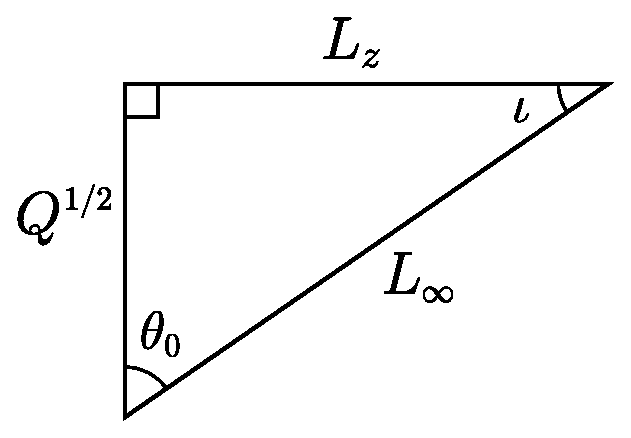
\includegraphics[width=0.25\textwidth]{./images/Triangle.eps}
    \caption{The angular momenta $L_\infty$, $L_z$ and $\sqrt{Q}$ define a right-angled triangle. The acute angles are $\theta_0$, the extremal value of the polar angle, and $\iota$, the orbital inclination \citep{Glampedakis2002}.\label{fig:L_triangle}}
\end{center}
\end{figure}
Introducing a second angular variable \citep{Drasco2004}
\begin{equation}
\xi = \xi_0\cos^2\chi.
\end{equation}
Over one $2\pi$ period of $\chi$, $\theta$ oscillates from its minimum value to its maximum and back. The geodesic equation for $\chi$ is
\begin{equation}
\varrho^2\diff{\chi}{\tau} = \sqrt{Q + L_z^2}.
\end{equation}

\section{Waveform Construction}\label{sec:Kludge}

We can now calculate the geodesic trajectory. The orbiting body is assumed to follow this track exactly; we ignore evolution due to the radiation of energy and angular momentum, which should be negligible for EMRBs. From this trajectory we calculate the waveform using a semirelativistic approximation \citep{Ruffini1981}: we assume the particle moves along the Kerr geodesic, but radiates as if it were in flat spacetime. This quick-and-dirty technique is known as a numerical kludge (NK), and has been shown to approximate well results computed by more accurate methods \citep{Babak2007}. It is often compared to a bead travelling along a wire. The shape of the wire is set by the Kerr geodesic, but the bead moves along in flat space.

\subsection{Kludge approximation}

Numerical kludge approximations aim to encapsulate the main characteristics of a waveform by using the exact particle trajectory (ignoring inaccuracies from radiative effects and from the particle's self-force), whilst saving on computational time by using approximate waveform generation techniques.

We build an equivalent flat-space trajectory by identifying the Boyer-Lindquist coordinates with a set of flat-space coordinates. We consider two choices:
\begin{enumerate}
\item Identify the Boyer-Lindquist coordinates with flat-space spherical polars $\{r\sub{BL},$ $\theta\sub{BL},$ $\phi\sub{BL}\} \rightarrow \{r\sub{sph}, \theta\sub{sph}, \phi\sub{sph}\}$, then define flat-space Cartesian coordinates \citep{Gair2005, Babak2007}
\begin{equation}
\boldsymbol{x} = \begin{pmatrix}
r\sub{sph} \sin\theta\sub{sph}\cos\phi\sub{sph} \\
r\sub{sph} \sin\theta\sub{sph}\sin\phi\sub{sph} \\
r\sub{sph} \cos\theta\sub{sph}
\end{pmatrix}.
\end{equation}
\item Identify the Boyer-Lindquist coordinates with flat-space oblate-spheroidal coordinates $\{r\sub{BL}, \theta\sub{BL}, \phi\sub{BL}\} \rightarrow \{r\sub{ob}, \theta\sub{ob}, \phi\sub{ob}\}$ so that the flat-space Cartesian coordinates are
\begin{equation}
\boldsymbol{x} = \begin{pmatrix}
\sqrt{{r\sub{ob}}^2 + a^2} \sin\theta\sub{ob}\cos\phi\sub{ob} \\
\sqrt{{r\sub{ob}}^2 + a^2} \sin\theta\sub{ob}\sin\phi\sub{ob} \\
r\sub{ob} \cos\theta\sub{ob}
\end{pmatrix}.
\end{equation}
These are appealing because in the limit that $G \rightarrow 0$, where the gravitating mass goes to zero, the Kerr metric in Boyer-Lindquist coordinates reduces to the Minkowski metric in oblate-spheroidal coordinates.
\end{enumerate}
The two coincide for $a \rightarrow 0$ or $r \rightarrow \infty$.

There is no well motivated argument that either coordinate system must yield an accurate GW; their use is justified {\it post facto} by comparison with results obtained from more accurate, and computationally intensive, methods \citep{Gair2005, Babak2007}. The ambiguity in assigning flat-space coordinates reflects the inconsistency of the semirelativistic approximation: the geodesic trajectory was calculated for the Kerr geometry; by moving to flat spacetime we lose the reason for its existence. This should not be regarded as a major problem; it is an artifact of the basic assumption that the shape of the trajectory is important for determining the character of the radiation, but the curvature of the spacetime in the vicinity of the source is not. By binding the particle to the exact geodesic, we ensure that the waveform has spectral components at the correct frequencies, but by assuming flat spacetime for generation of GWs they shall not have the correct amplitudes.

\subsection{Quadrupole-octupole formula}

Now we have a flat-space particle trajectory $x\sub{P}^\mu(\tau)$, we may apply a flat-space wave generation formula. We use the quadrupole-octupole formula to calculate the gravitational strain \citep{Bekenstein1973, Press1977, Yunes2008}
\begin{equation}
h^{jk}(t, \boldsymbol{x}) = -\frac{2G}{c^6r}\left(\ddot{I}^{jk} - 2n_i\ddot{S}^{ijk} + n_i\dddot{M}^{ijk}\right)_{t'\, =\, t - r/c},
\label{eq:octupole}
\end{equation}
where an over-dot represents differentiation with respect to time $t$, $t'$ is the retarded time, $r = \left|\boldsymbol{x} - \boldsymbol{x}\sub{P}\right|$ is the radial distance, $\boldsymbol{n}$ is the radial unit vector, and the mass quadrupole ${I}^{jk}$, current quadrupole ${S}^{ijk}$ and mass octupole ${M}^{ijk}$ are defined by
\begin{subequations}
\begin{align}
{I}^{jk}\left(t'\right) = {} & \intd{}{}{{x'}^j{x'}^kT^{00}\left(t', \boldsymbol{x'}\right) }{^3x'};\\
{S}^{ijk}\left(t'\right) = {} & \intd{}{}{{x'}^j{x'}^kT^{0i}\left(t', \boldsymbol{x'}\right)}{^3x'};\\
{M}^{ijk}\left(t'\right)  = {} & \recip{c}\intd{}{}{{x'}^i{x'}^j{x'}^kT^{00}\left(t', \boldsymbol{x'}\right)}{^3x'},
\end{align}
\end{subequations}
for energy-momentum tensor $T^{\mu\nu}$. This is correct for a slowly moving source. It is the familiar quadrupole formula \linebreak[0] (\citealt[section 36.10]{Misner1973}; \citealt[section 17.9]{Hobson2006}), derived from linearized theory, plus the next order terms. For a point mass, $T^{\mu\nu}$ contains a $\delta$-function which allows easy evaluation of the integrals.

Since we are only interested in GWs, we use the transverse-traceless (TT) gauge \citep[box 35.1]{Misner1973}.

\section{Signal detection and analysis}\label{sec:Signal}

\subsection{The LISA detector}\label{sec:Detector}

The classic LISA design is a three arm, space-borne laser interferometer \citep{Bender1998, Danzmann2003}. The arms form an equilateral triangle that rotates as the system's centre of mass follows a circular, heliocentric orbit, trailing $20^{\circ}$ behind the Earth. eLISA has a similar design, but  has only two arms, which are shorter in length, and trails $9^{\circ}$ behind the Earth \citep{Jennrich2011}.

To describe the detector configuration, and to transform from the MBH coordinate system to those of the detector, we use three coordinate systems: those of the BH at the GC $x_\bullet^i$; ecliptic coordinates centred at the solar system (SS) barycentre $x_\odot^i$, and coordinates that co-rotate with the detector $x\sub{d}^i$. The MBH's coordinate system and the SS coordinate system are depicted in \figref{BH_SS}.
\begin{figure}
\begin{center}
 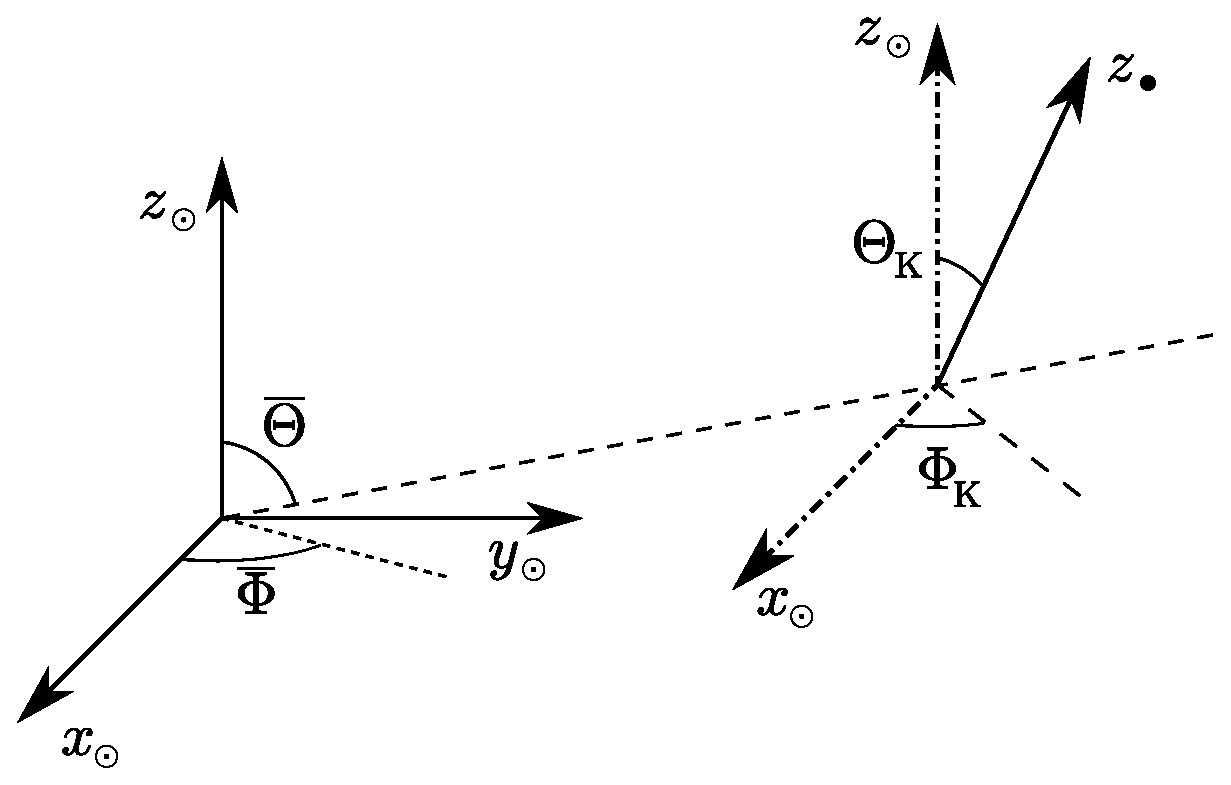
\includegraphics[width=0.42\textwidth]{./images/BH_SS_angles}
    \caption{The relationship between the MBH's coordinate system $x_\bullet^i$ and the SS coordinate system $x_\odot^i$. The MBH's spin axis is aligned with the $z_\bullet$-axis. The orientation of the MBH's $x$- and $y$-axes is arbitrary. We choose $x_\bullet$ to be orthogonal to the direction to the SS.}
   \label{fig:BH_SS}
\end{center}
\end{figure}
The mission geometry for LISA/eLISA is shown in \figref{SS_LISA}.
\begin{figure}
\begin{center}
 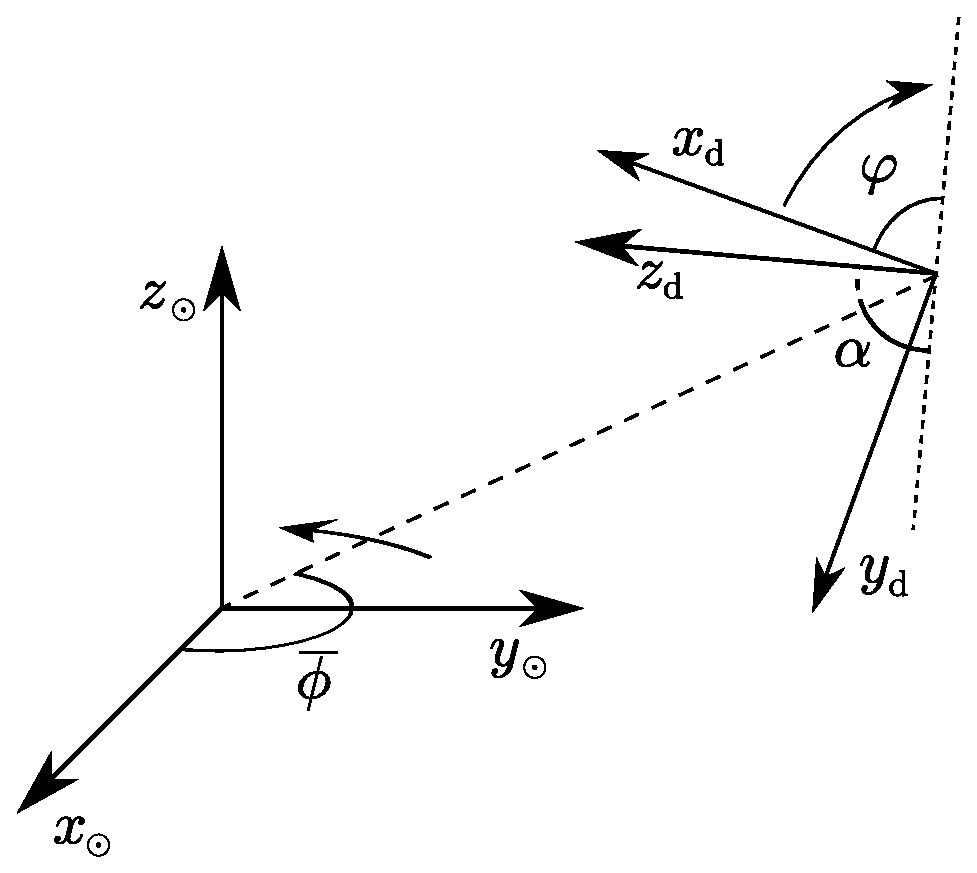
\includegraphics[width=0.32\textwidth]{./images/SS_LISA}
    \caption{The relationship between the detector coordinates $x\sub{d}^i$ and the ecliptic coordinates of the SS $x_\odot^i$ \citep{Bender1998, Jennrich2011}. The detector inclination is $\alpha = 60^{\circ}$.}
   \label{fig:SS_LISA}
\end{center}
\end{figure}
We define the detector coordinates such that the detector-arms lie in the $x\sub{d}$-$y\sub{d}$ plane as in \citet{Cutler1998}. We have computed the waveforms in the MBH's coordinates, but it is simplest to describe the measured signal using the detector's coordinates.

The strains measured in the three arms can be combined such that LISA behaves as a pair of $90^{\circ}$ interferometers at $45^{\circ}$ to each other, with signals scaled by ${\sqrt{3}}/{2}$ \citep{Cutler1998}. We denote the two detectors as I and II and use vector notation $\boldsymbol{h}(t) = \left(h\sub{I}(t), h\sub{II}(t)\right) = \left\{h_A(t)\right\}$ to represent signals from both detectors.

\subsection{Frequency domain formalism}

Having constructed the GW $\boldsymbol{h}(t)$ that shall be incident upon the detector, we may consider how to analyse the waveform and extract the information it contains. We briefly recap GW signal analysis, with application to LISA. A more complete discussion can be found in \citet{Finn1992} and \citet{Cutler1994}. Adaption for eLISA requires a substitution of the noise distribution, and the removal of the sum over data channels, since it would only have one.

The measured strain $\boldsymbol{s}(t)$ is the combination of the signal and the detector noise
\begin{equation}
\boldsymbol{s}(t) = \boldsymbol{h}(t) + \boldsymbol{n}(t);
\end{equation}
we assume the noise $n_A(t)$ is stationary and Gaussian, and that noise in the two detectors is uncorrelated, but shares the same characterisation \citep{Cutler1998}.

The properties of the noise allow us to define a natural inner product and associated distance on the space of signals \citep{Cutler1994}
\begin{equation}
\innerprod{\boldsymbol{g}}{\boldsymbol{k}} = 2\intd{0}{\infty}{\frac{\tilde{g}_A^\ast(f)\tilde{k}_A(f) + \tilde{g}_A(f)\tilde{k}_A^\ast(f)}{S\sub{n}(f)}}{f},
\label{eq:inner}
\end{equation}
introducing Fourier transforms
\begin{equation}
\tilde{g}(f) = \mathscr{F}\{g(t)\} = \intd{-\infty}{\infty}{g(t)\exp(2\pi i ft)}{t},
\end{equation}
and $S\sub{n}(f)$ is the noise spectral density. The signal-to-noise ratio is approximately
\begin{equation}
\rho[\boldsymbol{h}] = \innerprod{\boldsymbol{h}}{\boldsymbol{h}}^{1/2}.
\label{eq:SNR}
\end{equation}
The probability of a particular realization of noise $\boldsymbol{n}(t) = \boldsymbol{n}_0(t)$ is
\begin{equation}
p(\boldsymbol{n}(t) = \boldsymbol{n}_0(t)) \propto \exp\left[-\recip{2}\innerprod{\boldsymbol{n}_0}{\boldsymbol{n}_0}\right].
\end{equation}
Thus, if the incident waveform is $\boldsymbol{h}(t)$, the probability of measuring signal $\boldsymbol{s}(t)$ is
\begin{equation}
p(\boldsymbol{s}(t)|\boldsymbol{h}(t)) \propto \exp\left[-\recip{2}\innerprod{\boldsymbol{s}-\boldsymbol{h}}{\boldsymbol{s}-\boldsymbol{h}}\right].
\label{eq:sig_prob}
\end{equation}

\subsection{Noise curve}\label{sec:Noise}

LISA's noise has two sources: instrumental noise and confusion noise, primarily from WD binaries. The latter may be divided into contributions from galactic and extragalactic binaries. In this work we use the noise model of \citet{Barack2004}. The shape of the noise curve can be seen in \figref{Noise}. The instrumental noise dominates at both high and low frequencies. The confusion noise is important at intermediate frequencies, and is responsible for the cusp around $10^{-3}\units{Hz}$. eLISA shares the same sources of noise, but is less affected by confusion. Its sensitivity regime is shifted to higher frequencies because of the shorter arm length.
\begin{figure}[!htp]
\begin{center}
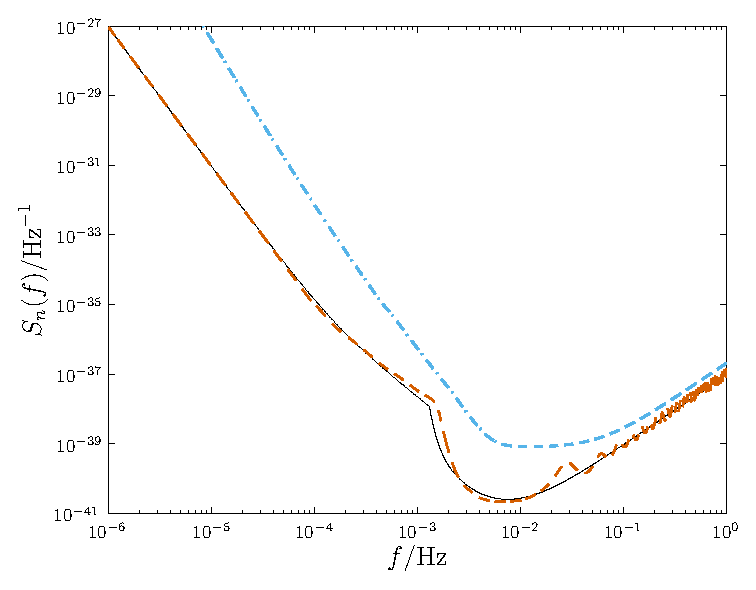
\includegraphics[width=0.6\textwidth]{./images/Fig_Noise}
\caption{The detector noise curves. The solid line indicates the analytic approximation of \citet{Barack2004} used in this work. For comparison, the dashed line is from the online LISA sensitivity curve generator (\url{http://www.srl.caltech.edu/~shane/sensitivity/}; \citealt*{Larson2000, Larson2002}). For bursts from the Galactic Centre we are most interested in the low-frequency region where the two curves are the same. The dot-dashed line shows the eLISA noise curve.\label{fig:Noise}}
\end{center}
\end{figure}

\subsection{Window functions}

There is one remaining complication regarding signal analysis: since we are Fourier transforming a finite signal we encounter spectral leakage; a contribution from large amplitude spectral components leaks into surrounding components (sidelobes), obscuring and distorting the spectrum at these frequencies \citep{Harris1978}. This is an inherent problem with finite signals; it shall be as much of a problem when analysing signals from an actual mission as it is computing waveforms here. To mitigate, but unfortunately not eliminate, these effects, the time-domain signal can be multiplied by a window function. We have adopted the Nuttall four-term window with continuous first derivative \citep{Nuttall1981} for the results presented here.

\section{Waveforms and detectability}\label{sec:Waveforms}

\subsection{Model parameters}

The waveform depends on the properties of the MBH; the CO and its orbit, and the detector.

We assume the position of the detector is known. This is specified by $\overline{\phi}$ and $\varphi$. We chose the initial position so $\overline{\phi} = 0$ when $\varphi = 0$ \citep{Cutler1998}; this does not qualitatively influence our results.

We also treat the sky position of the MBH, given by $\overline{\Theta}$ and $\overline{\Phi}$, as known. These are taken as the coordinates of Sgr A*, as the radio source is expected to be within $20 r\sub{g}$ of the MBH \citep{Reid2003,Doeleman2008}. We use the J2000.0 coordinates \citep{Reid1999, Yusef-Zadeh1999}. These change with time due to the rotation of the SS about the GC; the proper motion is about $6\units{mas\,yr^{-1}}$, mostly in the plane of the galaxy \citep{Reid1999, Backer1999, Reid2003}. The position is already determined to high accuracy and an EMRB can only give weak constraints on source position, hence we shall not try to infer it.\footnote{For comparison, an EMRI, which should be more informative, can only give sky localisation to $\sim 10^{-3}~\mathrm{steradians}$ \citep{Barack2004, Huerta2009}.}

For our model, the input parameters left to infer are:
\begin{enumerate}[leftmargin=*, widest=\:88--88.]
\item[1.] The MBH's mass $M_\bullet$. This is currently well constrained by the observation of stellar orbits about Sgr A* \citep{Ghez2008, Gillessen2009}, with the best estimate being $M_\bullet = (4.31 \pm 0.36) \times 10^6 M_\odot$. This depends upon the galactic centre distance $R_0$ as $M_\bullet = (3.95 \pm 0.06|\sub{stat} \pm 0.18|_{R_0, \, \mathrm{stat}} \pm  0.31|_{R_0, \, \mathrm{sys}}) \times 10^6 M_\odot (R_0 / 8\units{kpc})^{2.19}$, where the errors are statistical, independent of $R_0$; statistical from the determination of $R_0$, and systematic from $R_0$ respectively.
\item[2.] The spin parameter $a_\ast$. Naively this could be anywhere in the range $|a_\ast| < 1$; however it is possible to place an upper bound by contemplating spin-up mechanisms. Considering the torque from radiation emitted by an accretion disc, and swallowed by a BH, it can be shown that $|a_\ast| \lesssim 0.998$ \citep{Thorne1974}. Magnetohydrodynamical simulations of accretion discs produce a smaller maximum value of $|a_\ast| \sim 0.95$ \citep{Gammie2004}. The actual spin value could be much lower than this upper bound depending upon the MBH's evolution.
\item[3, 4.] The orientation angles for the black hole spin $\Theta\sub{K}$ and $\Phi\sub{K}$.
\item[5.] The ratio of the SS-GC distance $R_0$ and the CO mass $\mu$, which we denote as $\zeta = R_0/\mu$. This scales the amplitude of the waveform. Bursts, unlike inspirals, do not undergo orbital evolution, hence we cannot break the degeneracy in $R_0$ and $\mu$, and they cannot be inferred separately. The distance, like $M_\bullet$, is constrained by stellar orbits, the best estimate being $R_0 = 8.33 \pm 0.35\units{kpc}$ \citep{Gillessen2009}. The mass of the orbiting particle depends upon the type of object: whether it is an MS star, WD, NS or BH. Since we shall not know the $\mu$ precisely, we shall not be able to infer anything more about the distance to the GC.
\item[6, 7.] The angular momentum of the CO. This can be described using either $\{L_z, Q\}$ or $\{L_\infty, \iota\}$. We employ the latter, as the total angular momentum and inclination are less tightly correlated. Assuming spherical symmetry, we expect $\cos \iota$ to be uniformly distributed.
\item[8--10.] A set of coordinates to specify the trajectory. These could be positions at an arbitrary time. We use the angular phases at periapse, $\phi\sub{p}$ and $\chi\sub{p}$ (which determines $\theta\sub{p}$), as well as the time of periapse $t\sub{p}$.
\end{enumerate}
We are therefore interested in constraining $d = 10$ parameters.

\subsection{Waveforms}\label{sec:wave-ex}

\Figref{Examples} shows example waveforms to demonstrate some of the possible variations in the signal. All these assume the standard mass and position for the MBH as well as a $\mu = 10 M_\odot$ orbiting CO; other (randomly chosen) orbital parameters are specified in the captions. Radii are given in terms of the gravitational radius $r\sub{g} = GM_\bullet / c^2$.
\begin{figure}[!htp]
  \begin{center}
   \subfigure[{Waveform for $a_\ast \simeq 0.12$, $r\sub{p} \simeq 15.6 r\sub{g}$ and $\iota \simeq 2.1$. The SNR for the spherical polar kludge waveform (plotted) is $\rho[\boldsymbol{h}\sub{sph}] \simeq 451$, for the oblate-spheroidal kludge it is $\rho[\boldsymbol{h}\sub{ob}] \simeq 451$ (agreement to $0.01\%$).}]{\label{fig:Orbit_233} 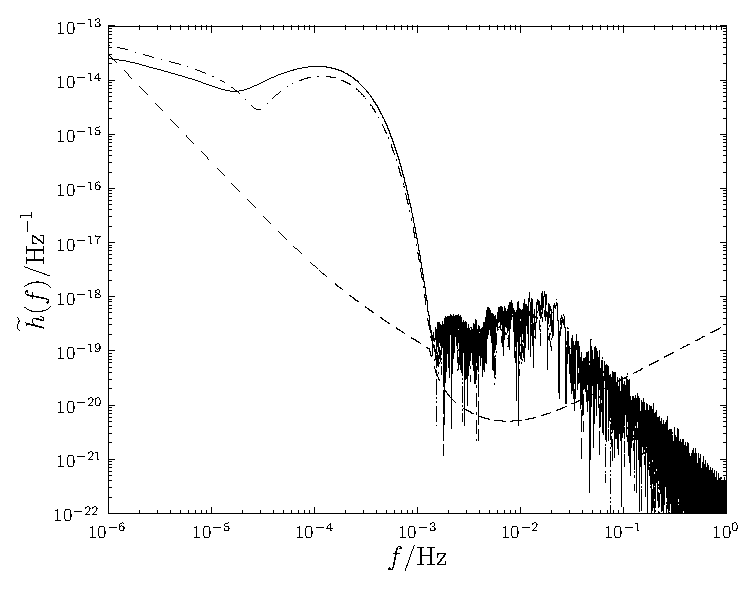
\includegraphics[width=0.47\textwidth]{./images/Fig_new_sph_h_233}} \quad
   \subfigure[{Waveform for $a_\ast \simeq 0.74$, $r\sub{p} \simeq 3.2 r\sub{g}$ and $\iota \simeq 1.2$. The SNR for the spherical polar kludge waveform (plotted) is $\rho[\boldsymbol{h}\sub{sph}] \simeq 70600$, for the oblate-spheroidal kludge it is $\rho[\boldsymbol{h}\sub{ob}] \simeq 74900$.}]{\label{fig:Orbit_135} 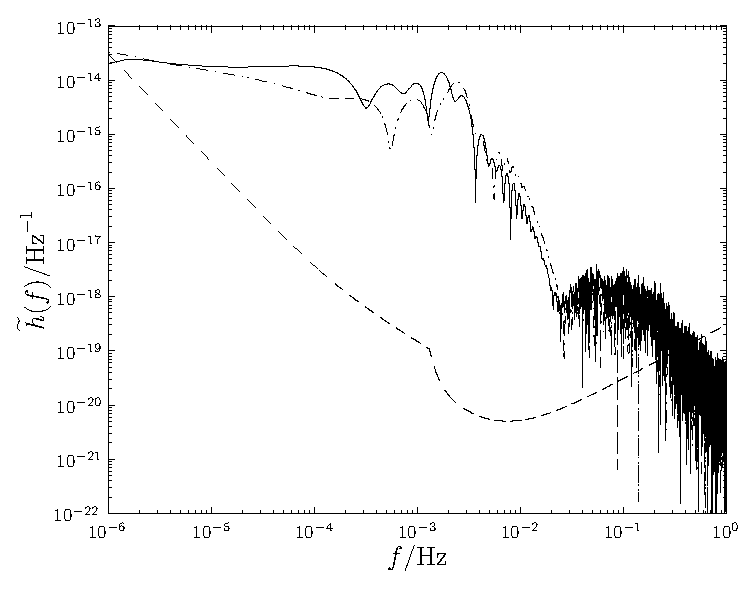
\includegraphics[width=0.47\textwidth]{./images/Fig_new_sph_h_135}}  
\caption{Example burst waveforms from the galactic centre. The strain $\widetilde{h}\sub{I}(f)$ is indicated by the solid line, $\widetilde{h}\sub{II}(f)$ by the dot-dashed line, and the noise curve by the dashed line. The kludge has been formulated using spherical polar coordinates.\label{fig:Examples}}
  \end{center}
\end{figure}

The plotted waveforms use the spherical polar coordinate system for the NK. Using oblate-spheroidal coordinates makes a small difference: on the scale shown here the only discernible difference would be in \figref{Orbit_135}; the maximum difference in the waveform (outside the high-frequency tail) is $\sim 10\%$. In the other cases the difference is entirely negligible (except in the high-frequency tail, which is not of physical significance). This behaviour is typical; for the closest orbits, with the most extreme spin parameters, the maximum difference in the waveforms may be $\sim 30\%$. The difference is largely confined to the higher frequency components, which are most sensitive to the parts of the trajectory closer to the MBH: the change in flat-space radius for the same Boyer-Lindquist radial coordinate causes a slight shift in the shape of the spectrum. Enforcing the same flat-space periapsis gives worse agreement across the spectrum.

To examine the effect of the coordinate choice, we compare SNRs calculated using the alternative schemes for a selection of orbits. The orbits have periapse distances uniformly distributed in log-space between the innermost orbit and $100 r\sub{g}$. Each had a spin and orbital inclination randomly chosen from distributions uniform in $a_\ast$ and $\cos \iota$.\footnote{The innermost orbit depends upon $a_\ast$ and $\iota$, hence these are drawn first.} For every periapse, five SNRs were calculated, each having a different set of intrinsic parameters specifying the relative orientation of the MBH, the orbital phase and the position of the detector, drawn from appropriate uniform distributions. We take the mean of $\ln \rho$ for each set of intrinsic parameters.\footnote{The logarithm is a better quantity to work with since the SNR is a positive-definite quantity that may be distributed over a range of magnitudes \citep[sections 22.1, 23.3]{MacKay2003}. Using median values yields results that are quantitatively similar.} The MBH parameters were fixed as for the GC.

The ratio of the two SNRs is shown in \figref{Oblate_sphere}.
\begin{figure}[!htp]
\begin{center}
 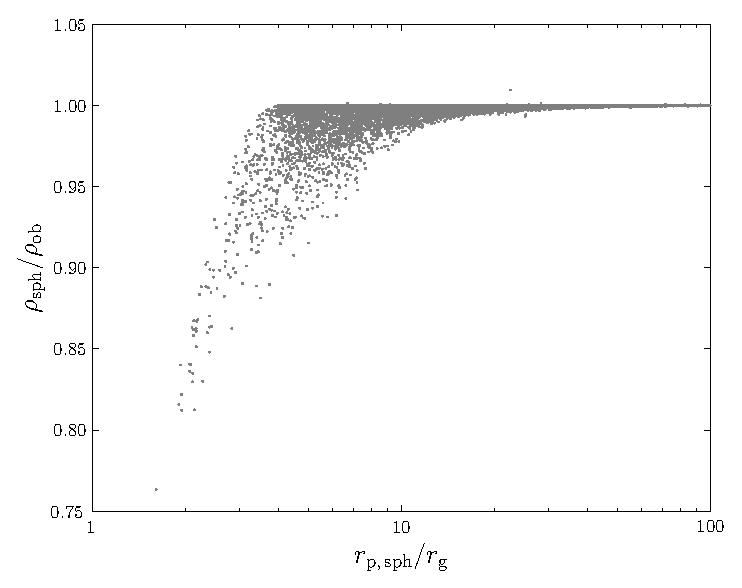
\includegraphics[width=0.6\textwidth]{./images/Fig_SNR_ratio}
 \caption{Ratio of SNR for a waveform calculated using spherical polar coordinates to that for a waveform using oblate-spheroidal coordinates.\label{fig:Oblate_sphere}}
   \end{center}
\end{figure}
The difference from the coordinate systems is only apparent for orbits with very small periapses. There is agreement to $10\%$ down to $r\sub{p} \simeq 4 r\sub{g}$; the maximal difference may be expected to be $\sim 20\%$, this is for periapses that are only obtainable for high spin values.

Since the deviation in the two waveforms is only apparent for small periapses, when the kludge approximation is least applicable, we conclude that the choice of coordinates is unimportant. The potential error of order $10\%$ is no greater than that inherent in the NK approximation (see \secref{Energy}). Without an accurate waveform template to compare against, we do not know if there is a preferable choice of coordinates. We adopt spherical coordinates for easier comparison with existing work.

\subsection{Signal-to-noise ratios}

The detectability of a burst depends upon its SNR. To characterise the variation of $\rho$ we calculated SNRs for a range of orbits. These were generated as in \secref{wave-ex}, we used $\sim 10^4$ different periapse distances.

The bursts were calculated for a $1 M_\odot$ CO. From \eqnref{octupole}, the amplitude of the waveform is proportional to the CO mass $\mu$, and so $\rho$ is also proportional to $\mu$; a $10 M_\odot$ object would be ten times louder on the same orbit. To make results mass independent, we work in terms of a mass-normalised SNR
\begin{equation}
\hat{\rho}[\boldsymbol{h}] = \left(\frac{\mu}{M_\odot}\right)^{-1}\rho[\boldsymbol{h}].
\end{equation}

There exists a correlation between the periapse radius and SNR, as shown in \figref{SNR}.
\begin{figure}[!htp]
  \begin{center}
  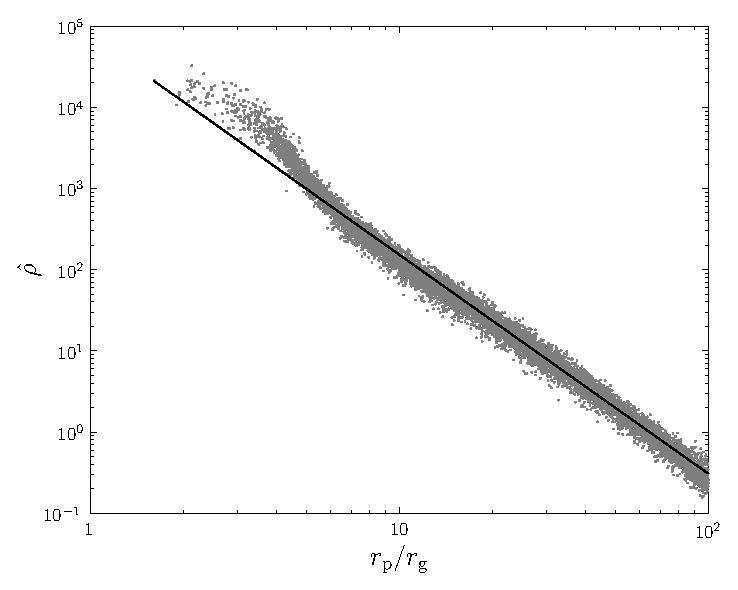
\includegraphics[width=0.6\textwidth]{./images/Fig_SNR}
    \caption{Mass-normalised SNR as a function of periapse radius. The plotted points are the values obtained by averaging over each set of intrinsic parameters. The best fit line is $\log(\hat{\rho}) = -2.69\log(r\sub{p}/r\sub{g}) + 4.88$. This is fitted to orbits with $r\sub{p} >  13.0 r\sub{g}$ and has a reduced chi-squared value of $\chi^2/\nu = 1.73$.\label{fig:SNR}}
  \end{center}
\end{figure}
Closer orbits produce louder bursts. To reflect this trend, we have fitted a simple fiducial power law,
\begin{equation}
\log\rho \simeq -2.7\log\left(\frac{r\sub{p}}{r\sub{g}}\right) + \log\left(\frac{\mu}{M_\odot}\right) + 4.9,
\label{eq:SNR-power-law}
\end{equation}
which is indicated by the straight line.\footnote{Using oblate-spheroidal coordinates instead of spherical polars gives a fit consistent to within $0.1\%$ as we have excluded the closest orbits.} This was done by maximising the likelihood, assuming $\ln \rho$ has a Gaussian distribution with standard deviation derived from the scatter because of variation in the intrinsic parameters. The power law is a good fit only for larger periapses. The shape is predominately determined by the noise curve. The change in the trend reflects the transition as from approximately power law behaviour to the bucket of the noise curve. Hence, we fit a power law to orbits with a characteristic frequency of $f_\ast = \sqrt{GM_\bullet/r\sub{p}} < 1 \times 10^{-3}\units{Hz}$, to avoid spilling into the bucket. Changing the cut-off within a plausible region alters the fit coefficients by around $0.1$.\footnote{The power law exponent $-2.7$ is inconsistent with $-13/4$ as predicted by the approximate model of \citet{Hopman2007}. This is the result of their approximate waveform model.}

The SNR shows no clear correlation with the other parameters (excluding $\mu$). However, the SNR is sensitive to the intrinsic parameters, in particular the initial position, and may vary by an order of magnitude.

Setting a threshold of $\rho = 10$, a $1 M_\odot$ ($10 M_\odot$) object would be expected to be detectable if the periapse distance is less than $27 r\sub{g}$ ($65 r\sub{g}$). \citet{Hopman2007}, assuming a threshold of $\rho = 5$, used an approximate form for the SNR based upon the quadrupole component of a circular orbit; their model, with updated parameters for the MBH, predicts bursts would be detectable out to $66 r\sub{g}$ ($135 r\sub{g}$). This is overly optimistic.

\section{Energy spectra}\label{sec:Energy}

To check the NK waveforms, we compare the energy spectra calculated from these with those obtained from the classic treatment of \citet{Peters1963} and \citet{Peters1964}. This calculates GW emission for Keplerian orbits in flat spacetime, assuming only quadrupole radiation. The spectrum produced should be similar to that obtained from the NK in weak fields, that is for large periapses; we do not expect an exact match because of the differing input physics and varying approximations.

In addition to using the energy spectrum, we also use the total energy flux. This contains less information than the spectrum; however, results have been calculated for parabolic orbits in Schwarzschild spacetime using time-domain black hole perturbation theory \citep{Martel2004}. These should be more accurate than results calculated using the Peters and Mathews formalism.

We do not intend to use the kludge waveforms to calculate an accurate energy flux: this would be inconsistent as we assume the orbits do not evolve with time. We only calculate the energy flux as a sanity check, to confirm that the kludge approximation is consistent with other approaches.

\subsection{Kludge spectrum}

A gravitational wave in the TT gauge has an effective energy-momentum tensor (\citealt{Misner1973}, section 35.15)
\begin{equation}
T_{\mu\nu} = \frac{c^4}{32\pi G}\left\langle\partial_\mu h_{ij} \partial_\nu h^{ij}\right\rangle,
\end{equation}
where $\langle\ldots\rangle$ indicates averaging over several wavelengths or periods. The energy flux through a sphere of radius $R$ is
\begin{equation}
\diff{E}{t} = \frac{c^3}{32\pi G} R^2 \int{\dd\Omega}\left\langle\diff{h_{ij}}{t}\diff{h^{ij}}{t}\right\rangle,
\end{equation}
with $\int{\dd\Omega}$ representing integration over all solid angles. From \eqnref{octupole} the waves have a $1/{r}$ dependence; if we define
\begin{equation}
h_{ij} = \frac{H_{ij}}{r},
\end{equation}
we see the flux is independent of $R$, as required for energy conservation, and
\begin{equation}
\diff{E}{t} = \frac{c^3}{32\pi G} \int{\dd\Omega}\left\langle\diff{H_{ij}}{t}\diff{H^{ij}}{t}\right\rangle.
\end{equation}
Integrating to find the total energy emitted
\begin{equation}
E = \frac{c^3}{32\pi G} \int{\dd\Omega}\int_{-\infty}^{\infty}{\dd t} \, \diff{H_{ij}}{t}\diff{H^{ij}}{t}.
\label{eq:integrate_E}
\end{equation}
Since we are considering all time, the localization of the energy is no longer of importance and it is unnecessary to average over several periods. Switching to Fourier representation $\widetilde{H}_{ij}(f) = \mathscr{F}\left\{H_{ij}(t)\right\}$,
\begin{equation}
E = \frac{\pi c^3}{4 G} \int{\dd\Omega}\int_{0}^{\infty}{\dd f} \, f^2 \widetilde{H}^{ij}(f)\widetilde{H}_{ij}^*(f),
\label{eq:total_E}
\end{equation}
using $\widetilde{H}_{ij}^*(f) = \widetilde{H}_{ij}(-f)$ as the signal is real. From this we identify the energy spectrum as
\begin{align}
\diff{E}{f} = \frac{\pi c^3}{4 G} \intd{}{}{}{\Omega} \, f^2 \widetilde{H}^{ij}(f)\widetilde{H}_{ij}^*(f).
\label{eq:NK_dEdf}
\end{align}

\subsection{Peters and Mathews spectrum}

For an orbit of eccentricity $e$ with periapse radius $r\sub{p}$, \citet{Peters1963} give the power radiated into the $n$th harmonic of the orbital angular frequency as
\begin{equation}
P(n) = \frac{32}{5}\frac{G^4}{c^5}\frac{M_\bullet^2\mu^2(M_\bullet + \mu)(1-e)^5}{r\sub{p}^5}g(n,e),
\label{eq:PM_P}
\end{equation}
where the function $g(n,e)$ is defined in terms of Bessel functions of the first kind
\begin{align}
g(n,e) = {} & \frac{n^4}{32}\left\{\left[J_{n-2}(ne) - 2eJ_{n-1}(ne) + \frac{2}{n}J_n(ne) + 2eJ_{n+1}(ne) - J_{n+2}(ne)\right]^2 \right. \nonumber \\*
 & + \left. \left(1 - e^2\right)\left[J_{n-2}(ne) - 2J_n(ne) + J_{n+2}(ne)\right]^2 + \frac{4}{3n^2}\left[J_n(ne)\right]^2\right\}.
% Line breaks follow Peters and Mathews paper
\end{align}
The Keplerian orbital frequency is
\begin{equation}
\omega_1^2 = \frac{G(M_\bullet + \mu)(1 - e)^3}{r\sub{p}^3} = (1 - e)^3\omega\sub{c}^2,
\label{eq:Kepler_freq}
\end{equation}
where $\omega\sub{c}$ is defined as the angular frequency of a circular orbit of radius $r\sub{p}$. The energy radiated per orbit into the $n$th harmonic, that is, at frequency $\omega_n = n\omega_1$, is
\begin{equation}
E(n) = \frac{2\pi}{\omega_1}P(n);
\label{eq:E(n)}
\end{equation}
as $e \rightarrow 1$ for a parabolic orbit, $\omega_1 \rightarrow 0$ as the orbital period becomes infinite. The energy radiated per orbit is then the total energy radiated. The spacing of harmonics is $\Delta\omega = \omega_1$, giving energy spectrum
\begin{equation}
\left.\diff{E}{\omega}\right|_{\omega_n}\omega_1 = E(n).
\end{equation}
Changing to linear frequency $2\pi f = \omega$,
\begin{align}
\left.\diff{E}{f}\right|_{f_n}  = {} & \frac{128\pi^2}{5}\frac{G^3}{c^5}\frac{M_\bullet^2\mu^2}{r\sub{p}^2}(1-e)^2g(n,e) \\*
  = {} & \frac{4\pi^2}{5}\frac{G^3}{c^5}\frac{M_\bullet^2\mu^2}{r\sub{p}^2}\ell(n,e),
\label{eq:PM_spectrum}
\end{align}
where the function $\ell(n,e)$ is defined in the last line. For a parabolic orbit, we must take the limit of $\ell(n,e)$ as $e \rightarrow 1$.

We simplify $\ell(n,e)$ using the recurrence formulae \citep[section 2.12]{Watson1995}
\begin{align}
J_{\nu-1}(z) + J_{\nu+1}(z)  = {} & \frac{2\nu}{z}J_\nu(z)\\*
J_{\nu-1}(z) - J_{\nu+1}(z)  = {} & 2J'_\nu(z),\label{eq:J_derivative}
\end{align}
and eliminate $n$ using
\begin{equation}
n = \frac{\omega_n}{\omega_1} = (1-e)^{-3/2}\tilde{f},
\end{equation}
where $\tilde{f} = \omega_n/\omega\sub{c} = f_n/f\sub{c}$ is a dimensionless frequency. To find the limit we define two new functions
\begin{equation}
A(\tilde{f}) = \lim_{e\rightarrow 1}\left\{\frac{J_n(ne)}{(1-e)^{1/2}}\right\}; \quad B(\tilde{f}) = \lim_{e\rightarrow 1}\left\{\frac{J'_n(ne)}{1-e}\right\}.
\end{equation}
To give a well-defined energy spectrum, both of these must be finite.

The Bessel function has an integral representation
\begin{equation}
J_\nu(z) = \recip{\pi}\intd{0}{\pi}{\cos(\nu\vartheta - z\sin\vartheta)}{\vartheta};
\end{equation}
we want the limit of this for $\nu \rightarrow \infty$, $z \rightarrow \infty$, with $z \leq \nu$. Using the stationary phase approximation, the dominant contribution to the integral comes from the regime in which the argument of the cosine is approximately zero \citep[sections 8.2, 8.43]{Watson1995}:
\begin{align}
J_\nu(z)  \sim {} & \recip{\pi}\intd{0}{\pi}{\cos\left(\nu\vartheta - z\vartheta + \frac{z}{6}\vartheta^3\right)}{\vartheta}\\*
  \sim {} & \recip{\pi}\intd{0}{\infty}{\cos\left(\nu\vartheta - z\vartheta + \frac{z}{6}\vartheta^3\right)}{\vartheta};
\end{align}
this last expression is an Airy integral and has a standard form \citep[section 6.4]{Watson1995}
\begin{equation}
\intd{0}{\infty}{\cos(t^3 + xt)}{t} = \frac{\sqrt{x}}{3}K_{1/3}\left(\frac{2x^{3/2}}{3^{3/2}}\right),
\end{equation}
where $K_\nu(z)$ is a modified Bessel function of the second kind. Using this to evaluate the limit gives
\begin{equation}
J_\nu(z) \sim \recip{\pi}\sqrt{\frac{2(\nu - z)}{3z}}K_{1/3}\left(\frac{2^{3/2}}{3}\sqrt{\frac{(\nu -z)^3}{z}}\right).
\label{eq:J_nu}
\end{equation}
For our case,
\begin{equation}
J_n(ne) \sim \recip{\pi}\sqrt{\frac{2}{3}}(1-e)^{1/2}K_{1/3}\left(\frac{2^{3/2}\tilde{f}}{3}\right),
\end{equation}
and the first limiting function is well defined,
\begin{equation}
A(\tilde{f}) = \recip{\pi}\sqrt{\frac{2}{3}}K_{1/3}\left(\frac{2^{3/2}\tilde{f}}{3}\right).
\end{equation}

To find the derivative we combine equations \eqref{eq:J_derivative} and \eqref{eq:J_nu}, and expand to lowest order yielding
\begin{align}
J'_n(ne) \sim {} & -\frac{1}{2\pi}\sqrt{\frac{2}{3}}(1-e)\left[2^{3/2}K'_{1/3}\left(\frac{2^{3/2}\tilde{f}}{3}\right) + \recip{\tilde{f}}K_{1/3}\left(\frac{2^{3/2}\tilde{f}}{3}\right)\right].
\end{align}
We may re-express the derivative using the recurrence formula \citep[section 3.71]{Watson1995}
\begin{equation}
K_{\nu-1}(z) + K_{\nu+1}(z) = -2K'_\nu(z)
\end{equation}
to give
\begin{align}
J'_n(ne)  \sim {} & \frac{1-e}{\sqrt{3}\pi}\left[K_{-2/3}\left(\frac{2^{3/2}\tilde{f}}{3}\right) + K_{4/3}\left(\frac{2^{3/2}\tilde{f}}{3}\right) - \recip{\sqrt{2}\tilde{f}}K_{1/3}\left(\frac{2^{3/2}\tilde{f}}{3}\right)\right].
\end{align}
And so finally we obtain the well-defined
\begin{align}
B(\tilde{f})  = {} & \recip{\sqrt{3}\pi}\left[K_{-2/3}\left(\frac{2^{3/2}\tilde{f}}{3}\right) + K_{4/3}\left(\frac{2^{3/2}\tilde{f}}{3}\right) - \recip{\sqrt{2}\tilde{f}}K_{1/3}\left(\frac{2^{3/2}\tilde{f}}{3}\right)\right].
\end{align}

Having obtained expressions for $A(\tilde{f})$ and $B(\tilde{f})$ in terms of standard functions, we can calculate the energy spectrum for a parabolic orbit. From \eqnref{PM_spectrum}
\begin{equation}
\diff{E}{f} = \frac{4\pi^2}{5}\frac{G^3}{c^5}\frac{M_\bullet^2\mu^2}{r\sub{p}^2}\ell\left(\frac{f}{f\sub{c}}\right),
\label{eq:PM_dEdf}
\end{equation}
where we have used the limit
\begin{align}
\ell(\tilde{f})  = {} & \left[8\tilde{f}^2B(\tilde{f}) - 2\tilde{f}A(\tilde{f})\right]^2 + \left(128\tilde{f}^4 + \frac{4\tilde{f}^2}{3}\right)\left[A(\tilde{f})\right]^2.
\label{eq:ell}
\end{align}
This agrees with the $e = 1$ result of \citet{Turner1977}, which was computed by direct integration along unbound orbits. \Figref{ell} shows how $\ell(n,e)$ changes with eccentricity including our result for a parabolic encounter. Although more power is radiated into higher harmonics, the peak of the spectrum does not move much: it is always between $f = f\sub{c}$ and $f = 2 f\sub{c}$, with $f = 2 f\sub{c}$ for $e = 0$ and $f \simeq 1.637 f\sub{c}$ for $e = 1$.
\begin{figure}[!htp]
\begin{center}
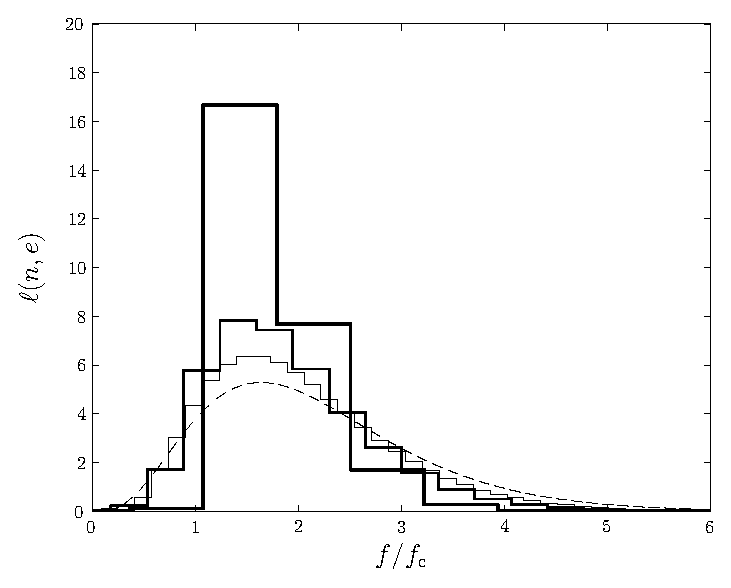
\includegraphics[width=0.6\textwidth]{./images/Fig_ell.eps}
\caption{The relative energy (per orbit) spectrum $\ell(n,e)$ for $e = 0.2$ (heavy line), $e = 0.5$ (medium line), $e = 0.7$ (light line), and the limiting result for $e = 1$ (dashed line) versus frequency. Compare with figure 3 of \citet{Peters1963}.\label{fig:ell}}
\end{center}
\end{figure}

\subsubsection{Total Energy}

To check the validity of this limit we can calculate the total energy radiated by integrating \eqnref{PM_dEdf} over all frequencies, or by summing the energy radiated into each harmonic. These must yield the same result. Summing:
\begin{equation}
E\sub{sum} = \frac{64\pi}{5}\frac{G^3}{c^5}\frac{M_\bullet^2\mu^2}{r\sub{p}^2}\omega\sub{c}(1-e)^{7/2}\sum_n g(n,e),
\end{equation}
where we have used equations \eqref{eq:PM_P}, \eqref{eq:Kepler_freq} and \eqref{eq:E(n)}. \citet{Peters1963} provide the result
\begin{equation}
\sum_n g(n,e) = \frac{1 + (73/24)e^2 + (37/96)e^4}{(1-e^2)^{7/2}}.
\end{equation}
Using this,
\begin{equation}
E\sub{sum} = \frac{64\pi}{5}\frac{G^3}{c^5}\frac{M_\bullet^2\mu^2}{r\sub{p}^2}\omega\sub{c}\frac{1 + (73/24)e^2 + (37/96)e^4}{(1+e)^{7/2}},
\end{equation}
which is perfectly well behaved as $e \rightarrow 1$,
\begin{equation}
E\sub{sum} = \frac{85\pi}{2^{5/2}3}\frac{G^3}{c^5}\frac{M_\bullet^2\mu^2}{r\sub{p}^2}\omega\sub{c}.
\label{eq:PM_total}
\end{equation}
Integrating the energy spectrum \eqnref{PM_dEdf} gives
\begin{equation}
E\sub{int} = \frac{2\pi}{5}\frac{G^3}{c^5}\frac{M_\bullet^2\mu^2}{r\sub{p}^2}\omega\sub{c}\intd{0}{\infty}{\ell(\tilde{f})}{\tilde{f}}.
\end{equation}
The integral can be evaluated numerically as
\begin{equation}
\intd{0}{\infty}{\ell(\tilde{f})}{\tilde{f}} = 12.5216858\ldots = \frac{425}{2^{7/2}3}.
\end{equation}
The two total energies are consistent, $E\sub{int} = E\sub{sum}$.

\subsection{Comparison}

Two energy spectra are plotted in \figref{Energy} for orbits with periapses of $r\sub{p} = 15.0 r\sub{g}$, $30.0 r\sub{g}$ and $60.0 r\sub{g}$.
\begin{figure}[!htp]
  \begin{center}
   \subfigure[$r\sub{p} = 15.0 r\sub{g}$, log-log plot.]{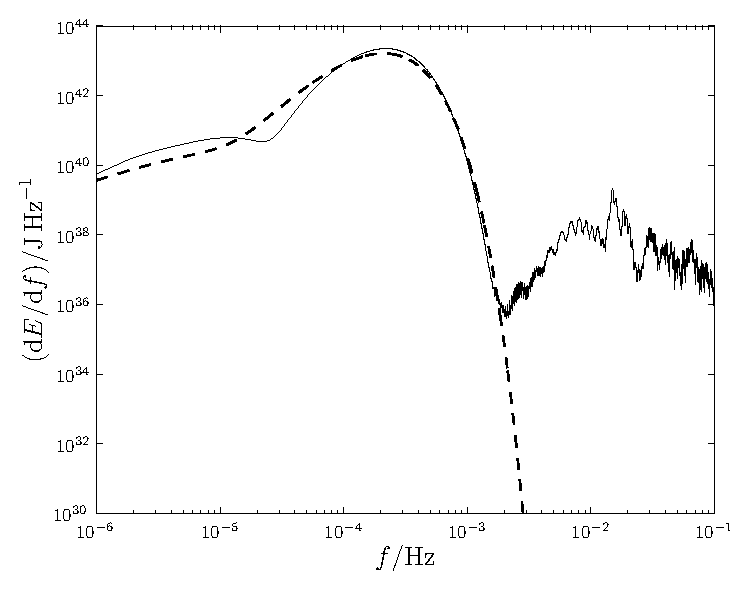
\includegraphics[width=0.47\textwidth]{./images/Fig_Loglog_E_15}} \quad
   \subfigure[$r\sub{p} = 15.0 r\sub{g}$, log-linear plot.]{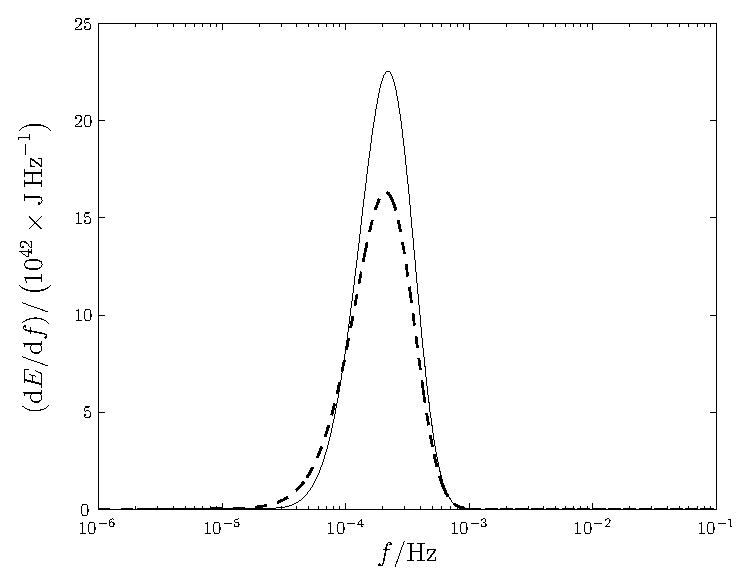
\includegraphics[width=0.47\textwidth]{./images/Fig_Loglin_E_15}} \\
   \subfigure[$r\sub{p} = 30.0 r\sub{g}$, log-log plot.]{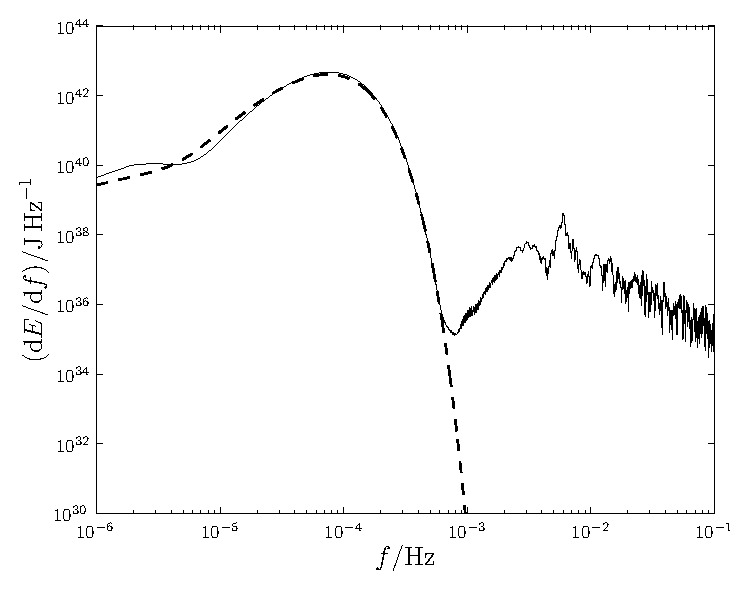
\includegraphics[width=0.47\textwidth]{./images/Fig_Loglog_E_30}} \quad
   \subfigure[$r\sub{p} = 30.0 r\sub{g}$, log-linear plot.]{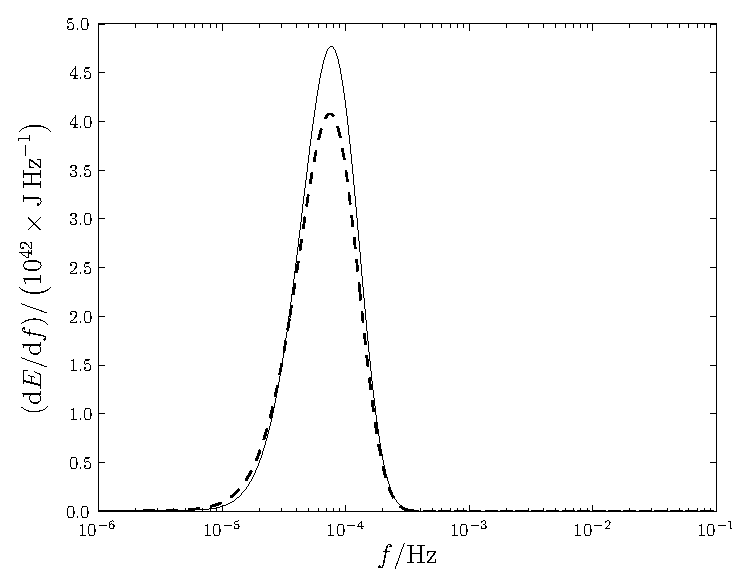
\includegraphics[width=0.47\textwidth]{./images/Fig_Loglin_E_30}} \\
   \subfigure[$r\sub{p} = 60.0 r\sub{g}$, log-log plot.]{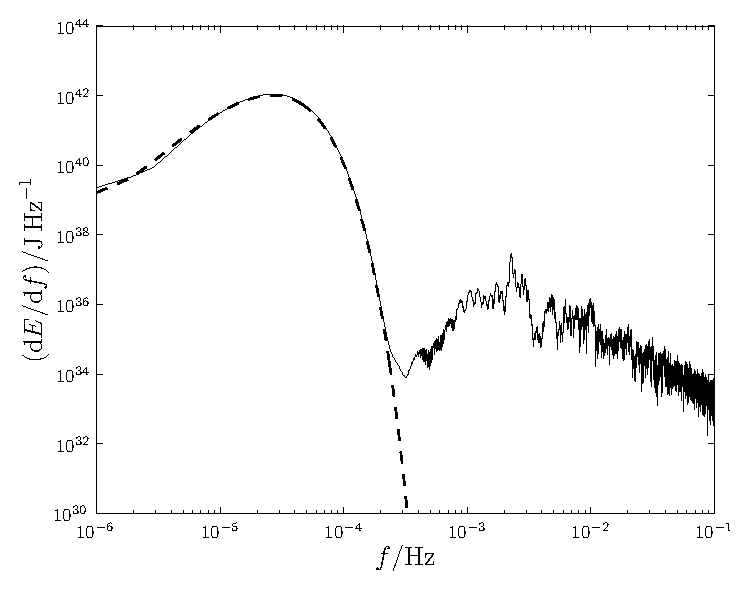
\includegraphics[width=0.47\textwidth]{./images/Fig_Loglog_E_60}} \quad
   \subfigure[$r\sub{p} = 60.0 r\sub{g}$, log-linear plot.]{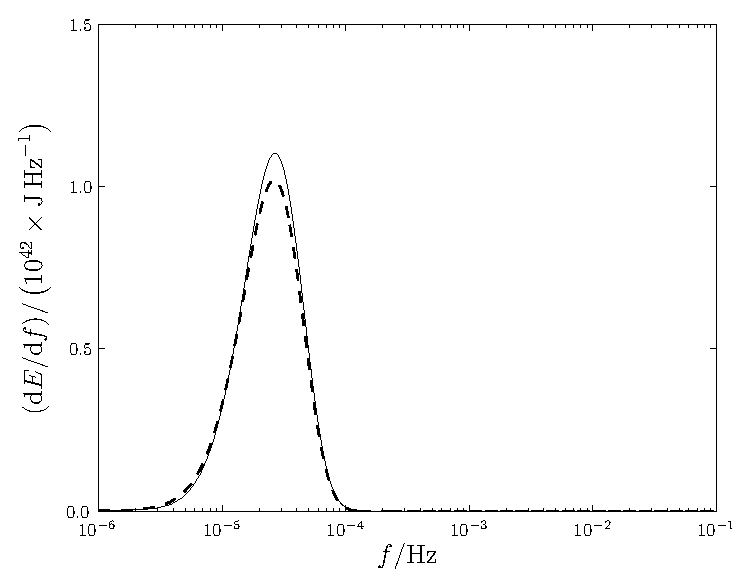
\includegraphics[width=0.47\textwidth]{./images/Fig_Loglin_E_60}}
    \caption{Energy spectra for a parabolic orbit of a $\mu = 10 M_\odot$ object about a Schwarzschild BH with $M_\bullet = 4.31 \times 10^6 M_\odot$. The spectra calculated from the NK waveform is shown by the solid line and the Peters and Mathews flux is indicated by the dashed line. The NK waveform includes octupole contributions. The high frequency tail is the result of spectral leakage.\label{fig:Energy}}
  \end{center}
\end{figure}
The two spectra appear to be in good agreement, showing the same general shape in the weak-field limit. The NK spectrum is more tightly peaked, but is always within a factor of $2$ at the apex. The peak of the spectrum is shifted to a marginally higher frequency in the NK spectrum primarily because of the addition of the current quadrupole and mass octupole terms.

Comparing the total energy fluxes, ratios of the various energies are plotted in \figref{Energy_ratio}.
\begin{figure}[!htp]
  \begin{center}
   \subfigure[Versus periapsis]{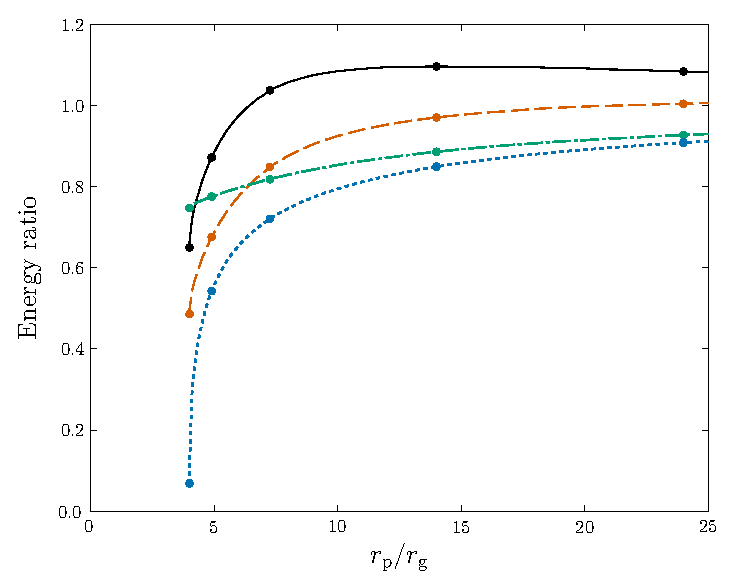
\includegraphics[width=0.475\textwidth]{./images/Fig_Energy_ratio_peri}} \quad
   \subfigure[Versus amount of rotation]{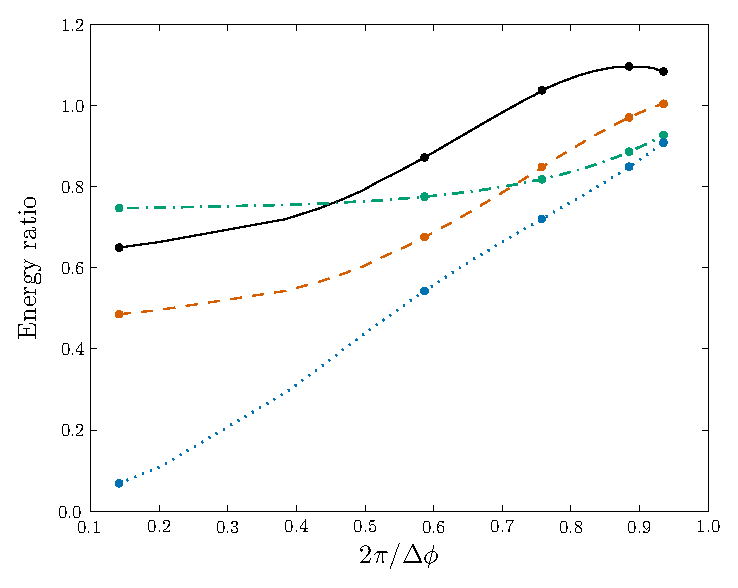
\includegraphics[width=0.475\textwidth]{./images/Fig_Energy_ratio_orbit}}
    \caption{Ratios of energies as a function of periapsis $r\sub{p}$ and $2\pi$ divided by the total angle of rotation in one orbit $\Delta\phi$ ($2\pi/\Delta\phi = 1$ for a Keplerian orbit). The solid line shows the ratio of the numerical kludge and Martel energies $E\sub{NK}/E\sub{M}$; the dashed line shows the ratio of the NK energy calculated using only the mass quadrupole term and the Martel energy $E\sub{NK(Q)}/E\sub{M}$; the dot-dashed line shows the ratio of the quadrupole and quadrupole-octupole NK energies $E\sub{NK(Q)}/E\sub{NK}$, and the dotted line shows the ratio of the Peters and Mathews and quadrupole NK energies $E\sub{PM}/E\sub{NK(Q)}$. The spots show the mapping between the two abscissa scales. Compare with figure 4 of \citet{Gair2005}.\label{fig:Energy_ratio}}
  \end{center}
\end{figure}
We introduce an additional energy here, the quadrupole NK energy $E\sub{NK(Q)}$. This allows easier comparison with the Peters and Mathews energy which includes only quadrupole radiation. It can be calculated in three ways:
\begin{enumerate}
\item Inserting the waveform $\widetilde{h}(f)$ generated including only the mass quadrupole term in \eqnref{octupole} into \eqnref{total_E} and integrating. This is equivalent to the method used to calculate $E\sub{NK}$.
\item Numerically integrating the quadrupole GW luminosity (\citealt{Misner1973}, section 36.7; \citealt{Hobson2006}, section 18.7)
\begin{equation}
E = \frac{G}{5c^9}\intd{}{}{\dddot{\Ibar}_{ij}\dddot{\Ibar}^{ij}}{t},
\label{eq:E_quad}
\end{equation}
where $\Ibar_{ij} = I_{ij} - (1/3)I\delta_{ij}$ is the reduced mass quadrupole tensor. We can obtain this from \eqnref{integrate_E}, by integrating over all angles when the waveform only contains the mass quadrupole component. This has the advantage of avoiding the effects of spectral leakage or the influence of window functions.
\item Using the analytic expressions for the integral \eqnref{E_quad} given in appendix A of \citet{Gair2005}.
\end{enumerate}
All three agree to within computational error. No difference is visible on the scale plotted in \figref{Energy_ratio}. This demonstrates the validity of the code.

We have used the amount of rotation $\Delta\phi$ as a convenient measure for the abscissa. For an equatorial orbit in Kerr spacetime,
\begin{align}
\Delta\phi  = {} & 2\intd{r\sub{p}}{\infty}{\diff{\phi}{r}}{r} = \sqrt{\frac{2}{M_\bullet}}L_z\intd{r\sub{p}}{\infty}{\frac{r^2 - 2M_\bullet(1 - a/L_z)r}{(r^2 - 2M_\bullet r + a^2)w}}{r},
\end{align}
where
\begin{equation}
w^2 = r^3 - \frac{L_z^2}{2M_\bullet}r^2 + (L_z - a)^2r;
\end{equation}
$L_z$ is the specific angular momentum about the $z$-axis; $a$ is the spin parameter, and we have adopted units with $G = c = 1$. We shall find it useful to define
\begin{equation}
r_\pm = M_\bullet \pm \sqrt{M_\bullet^2 - a^2},
\end{equation}
and the two nonzero roots of the cubic $w^2$
\begin{equation}
r_{\mathrm{p},\,1} = \frac{L_z^2}{4M_\bullet} \pm \sqrt{\frac{L_z^4}{16M_\bullet^2} - (L_z -a)^2};
\end{equation}
the periapsis is the larger root $r\sub{p} > r_1$. This equation implicitly gives $L_z$ as a function of $r\sub{p}$. The integral may be rewritten as
\begin{equation}
\Delta\phi = \sqrt{\frac{2}{M}}L_z\intd{r\sub{p}}{\infty}{\recip{w}\left(1 + \frac{\alpha_+}{r-r_+} + \frac{\alpha_-}{r-r_-}\right)}{r},
\end{equation}
where
\begin{equation}
\alpha_\pm = \pm\frac{2Mar_\pm - a^2L_z}{2L_z\sqrt{M^2-a^2}}.
\end{equation}
This may be evaluated using elliptic integrals \citep[3.131.8, 3.137.8]{Gradshteyn2000}
\begin{equation}
\Delta\phi = 2 L_z \sqrt{\frac{2}{r\sub{p}M}}\left[\frac{\alpha_+}{r_+}\Pi\left(\frac{r_+}{r\sub{p}}\middle|\frac{r_1}{r\sub{p}}\right) + \frac{\alpha_-}{r_-}\Pi\left(\frac{r_-}{r\sub{p}}\middle|\frac{r_1}{r\sub{p}}\right)\right],
\end{equation}
where $\Pi(n|m) = \int_{0}^{\pi/2}{\dd\vartheta/(1-n\sin^2\vartheta)\sqrt{1-m\sin^2\vartheta}}$ is the complete elliptic integral of the third kind. In the limit of $a \rightarrow 0$ we recover the Schwarzschild result \citep{Cutler1994}
\begin{equation}
\Delta\phi =  2 L_z\sqrt{\frac{2}{r\sub{p}M}}K\left(\frac{r_1}{r\sub{p}}\right),
\end{equation}
where $K(m) = \int_{0}^{\pi/2}{\dd\vartheta/\sqrt{1-m\sin^2\vartheta}}$ is the complete elliptic integral of the first kind.

The ratios all tend towards one in the weak field, as required, but differences become more pronounced in the strong field. The NK energy is larger than the Peters and Mathews result $E\sub{PM}$. This behaviour has been seen before for high eccentricity orbits about a non-spinning BH \citep{Gair2005}. It may be explained by considering the total path length for the different orbits: the Peters and Mathews spectrum assumes a Keplerian orbit, the orbit in Kerr geometry rotates more than this. The greater path length leads to increased emission of gravitational waves and a larger energy flux. Our bead must travel further along its wire. A good proxy for the path length is the angle of rotation $\Delta\phi$; this is $2\pi$ for a Keplerian orbit, in Kerr the angle should be $2\pi$ in the limit of an infinite periapsis, whereas for a periapsis small enough that the orbit shows zoom-whirl behaviour, the total angle may be many times $2\pi$. There is a reasonable correlation between the amount of rotation $2\pi/\Delta\phi$ and the ratio of energies.

Error in the NK energy compared with the time-domain black hole perturbation theory results of Martel comes from two sources: the neglecting of higher order multipole contributions and the ignoring of background curvature. The contribution of the former can be estimated by looking at the difference in the NK energy by including the current quadrupole and mass octupole terms. From \figref{Energy_ratio} we see that these terms give a negligible contribution in the weak field, but the difference is $\sim20\%$ in the strong field. This explains why the Martel energy $E\sub{M}$ is greater in the strong field, as it includes contributions from all multipoles. Neglecting the background curvature increases the NK energy relative to $E\sub{M}$. This partially cancels out the error introduced by not including higher order terms: this accidentally leads to $E\sub{NK(Q)}$ being more accurate than $E\sub{NK}$ for $r\sub{p} \gtrsim 10 r\sub{g}$ \citep{Tanaka1993}.

From the level of agreement we may be confident that the NK waveforms are a reasonable approximation. The difference in energy flux is only greater than $10\%$ for very strong fields $r\sub{p} \simeq 4 r\sub{g}$; since this is dependent on the square of the waveform, typical accuracy in the waveform may be $\sim 5\%$ \citep{Gair2005,Tanaka1993}. This is more significant than the variation in waveforms we generally found using the two alternative coordinate systems for the NK (in this case the two coincide because $a_\ast = 0$).

\section{Parameter estimation}\label{sec:Estimation}

Having detected a signal, we are interested in what we can learn about the source. We have an inference problem that can be solved by  application of Bayes' Theorem (\citealt{Jaynes2003}, chapter 4): the probability distribution for our parameters given that we have detected the signal $\boldsymbol{s}(t)$ is given by the posterior
\begin{equation}
p(\boldsymbol{\lambda}|\boldsymbol{s}(t)) = \frac{p(\boldsymbol{s}(t)|\boldsymbol{\lambda})p(\boldsymbol{\lambda})}{p(\boldsymbol{s}(t))}.
\end{equation}
Here $p(\boldsymbol{s}(t)|\boldsymbol{\lambda})$ is the likelihood of the parameters, $p(\boldsymbol{\lambda})$ is the prior probability distribution for the parameters, and the evidence $p(\boldsymbol{s}(t)) = \intd{}{}{p(\boldsymbol{s}(t)|\boldsymbol{\lambda})}{^d \lambda}$ is, for our purposes, a normalising constant. The likelihood depends upon the realization of noise. If parameters $\boldsymbol{\lambda}_0$ define a waveform $\boldsymbol{h}_0(t) = \boldsymbol{h}(t; \boldsymbol{\lambda}_0)$, the probability that we observe signal $\boldsymbol{s}(t)$ GW is given by \eqnref{sig_prob}, so the likelihood is
\begin{equation}
p(\boldsymbol{s}(t)|\boldsymbol{\lambda}_0) \propto \exp\left[-\recip{2}\innerprod{\boldsymbol{s}-\boldsymbol{h}_0}{\boldsymbol{s}-\boldsymbol{h}_0}\right].
\label{eq:likelihood}
\end{equation}
If we were to define this as a probability distribution for the parameters $\boldsymbol{\lambda}$, the modal values are the maximum-likelihood (ML) parameters $\boldsymbol{\lambda}\sub{ML}$. The waveform $\boldsymbol{h}(t; \boldsymbol{\lambda}\sub{ML})$ is the signal closest to $\boldsymbol{s}(t)$, where distance is defined using the inner product \eqnref{inner} \citep{Cutler1994}.

To discover if any parameters can be accurately inferred, we must characterise the form of the posterior. To map out the posterior we employ a Markov chain Monte Carlo (MCMC) approach.

\subsection{Markov chain Monte Carlo methods}

MCMC methods are widely used for inference problems; they are a family of algorithms for integrating over complicated distributions and are efficient for high-dimensional problems \citep[chapter 29]{MacKay2003}. Parameter space is explored by constructing a chain of $N$ samples. The distribution of points visited by the chain maps out the underlying distribution; this becomes asymptotically exact as $N \rightarrow \infty$. Samples are added sequentially, if the current state is $\boldsymbol{\lambda}_n$ a new point $\boldsymbol{\lambda}^\ast$ is drawn and accepted with probability
\begin{equation}
\mathcal{A} = \min\left\{\frac{\pi(\boldsymbol{\lambda}^\ast)\mathcal{L}(\boldsymbol{\lambda}^\ast)\mathcal{Q}(\boldsymbol{\lambda}_n;\,\boldsymbol{\lambda}^\ast)}{\pi(\boldsymbol{\lambda}_n)\mathcal{L}(\boldsymbol{\lambda}_n)\mathcal{Q}(\boldsymbol{\lambda}_n;\,\boldsymbol{\lambda}^\ast)}, 1\right\},
\end{equation}
setting $\boldsymbol{\lambda}_{n + 1} = \boldsymbol{\lambda}^\ast$, where $\mathcal{L}(\boldsymbol{\lambda})$ is the likelihood, in our case from \eqnref{likelihood}; $\pi(\boldsymbol{\lambda})$ is the prior, and $\mathcal{Q}$ is a proposal distribution. If the move is not accepted  $\boldsymbol{\lambda}_{n + 1} = \boldsymbol{\lambda}_n$. This is the Metropolis-Hastings algorithm \citep{Metropolis1953,Hastings1970}.

Waiting long enough yields an exact posterior, but it is desirable for the MCMC to converge quickly. This requires a suitable choice for the proposal distribution, which can be difficult, since we do not yet know the shape of the target distribution.

One method to define the proposal is to use the previous results in the chain and refine $\mathcal{Q}$ by learning from these. Such approaches are known as adaptive methods. Updating using previous points means that the chain is no longer Markovian. Care must be taken to ensure that ergodicity is preserved and convergence obtained \citep{Roberts2007,Andrieu2008}. To avoid this complication, we follow \citet{Haario1999}, and use the adapting method as a burn in phase. We have an initial phase where the proposal is updated based upon accepted points. After this we fix the proposal and proceed as for a standard MCMC. By only using samples from the second part, we guarantee that the chain is Markovian and ergodic, whilst still enjoying the benefits of a tailor-made proposal. After only a finite number of samples we cannot assess the optimality of this \citep{Andrieu2008}, but the method is still effective.

To tune $\mathcal{Q}$, we use an approach based upon the adaptive Metropolis algorithm \citep{Haario2001}. The proposal is taken to be a multivariate normal distribution centred upon the current point, the covariance of which is
\begin{equation}
\boldsymbol{C} = s \left(\boldsymbol{V}_n + \varepsilon\boldsymbol{C}_0\right),
\end{equation}
where $\boldsymbol{V}_n$ is the covariance of the accepted points $\{\boldsymbol{\lambda}_1,\ldots,\boldsymbol{\lambda}_n\}$, $s$ is a scaling factor that controls the step size, $\varepsilon$ is a small positive constant (typically $0.0025$), and $\boldsymbol{C}_0$ is a constant matrix included to ensure ergodicity.

Our adaptation is run in three phases. The initial phase is to get the chain moving. For this $\boldsymbol{C}_0\super{init}$ is a diagonal matrix with elements calibrated from initial one dimensional MCMCs. This finishes after $N\sub{init}$ accepted points.

For the second phase, we use the proposal covariance from the initial phase $\boldsymbol{C}\super{init}$ for $\boldsymbol{C}_0\super{main}$. We reset the covariance of the accepted points so that it only includes points from this phase. This is the main adaptation phase and lasts until $N\sub{main}$ points have been accepted.

In the final adaptation phase we restart the chain at the true parameter values. We no longer update the shape of the covariance ($\boldsymbol{V}_n$ remains fixed), but adjust the step size $s$ to tune the acceptance rate; it is then fixed, along with everything else, for the final MCMC.

Throughout the adaptation, we update the step size $s$ after every $100$ trial points (whether or not they are accepted). While updating, the covariance $\boldsymbol{V}_n$ changes after every $1000$ trial points. We set $N\sub{init} = 50000$ and $N\sub{main} = 450000$.

We initially aimed for an acceptance rate of $0.234$; this is optimal for a random walk Metropolis algorithm with some specific high-dimensional target distributions \citep{Roberts1997,Roberts2001}. In many cases we found better convergence when aiming for a lower acceptance rate, say $0.1$. This is not unexpected: the optimal rate may be lower than $0.234$ when the parameters are not independent and identically distributed \citep{Bedard2007, Bedard2008, Bedard2008a}. In practice, the final acceptance rate is (almost always) lower than the target rate as the use of a multivariate Gaussian for the proposal distribution is rarely a good fit at the edges of the posterior. Consequently, the precise choice for the target acceptance rate is unimportant as long as it is of the correct magnitude. Final rates are typically within a factor of $2$ of the target value. As an initial choice, we set $s = 2.38^2/d$, which is the optimal choice if $\boldsymbol{C}$ was the true target covariance for a high dimensional target of independent and identically distributed parameters \citep{Gelman1996,Roberts1997,Roberts2001,Haario2001}.\footnote{Reasonably good results may be obtained by fixing $s$ at this value, and not adjusting to fine tune the acceptance rate.}

To assess the convergence of the MCMC we check the trace plot (the parameters values throughout the run) for proper mixing, that the one and two dimensional posterior plots fill out to a smooth distribution, and that the distribution widths tend towards consistent values.

\section{Results}\label{sec:Results}

\subsection{Data set}

To investigate the information contained in EMRBs, we again considered a range of orbits. The MBH was assumed to have the standard mass and position. The CO was chosen to be $10 M_\odot$, as the most promising candidates for EMRBs would be BHs: they are massive and hence produce higher SNR bursts, they are more likely to be on close orbits as a consequence of mass segregation \citep{Bahcall1977, Alexander2009}, and they cannot be tidally disrupted.

Orbits were chosen with periapses uniformly distributed in logarithmic space between the the inner-most orbit and $16 r\sub{g}$. The other parameters were chosen randomly from appropriate uniform distributions. 

The results of the MCMC runs show strong and complex parameter dependencies. Some example results are shown in \figref{MCMC-1}, \ref{fig:MCMC-2} and \ref{fig:MCMC-3}.
\begin{figure}[!htp]
\begin{center}
   \includegraphics[width=0.95\textwidth]{./images/Fig_MCMC_327_triangle_40}
\caption{Marginalised one and two dimensional posteriors. The scales are identical in both sets of plots. The dotted line indicates the true value. These distributions are fairly cromulent and well converged. Angular momentum is in units of $L_\bullet = GM_\bullet c^{-1}$. The input orbit has $r\sub{p} \simeq 8.54 r\sub{g}$ and $\rho \simeq 916$.\label{fig:MCMC-1}}
\end{center}
\end{figure}

The first is well-behaved. It is almost Gaussian, but we see some asymmetries and imperfections. There are also strong degeneracies, indicated by needle-like distributions. This is a fairly standard example: there are runs which are closer to being Gaussian (especially at higher SNR), and equally there are tighter correlations. The lenticular $M_\bullet$--$L_\infty$ degeneracy is common.

\begin{figure}[!htp]
\begin{center}
   \includegraphics[width=0.95\textwidth]{./images/Fig_MCMC_53_triangle_40}
\caption{Marginalised one and two dimensional posteriors. The scales are identical in both sets of plots. The dotted line indicates the true value. These distributions show definite non-gaussianity. The input orbit has $r\sub{p} \simeq 9.86 r\sub{g}$ and $\rho \simeq 1790$.\label{fig:MCMC-2}}
\end{center}
\end{figure}

The second shows banana-like degeneracies. These are not uncommon; there are varying degrees of curvature. The more complicated shape makes it harder for the MCMC to converge, so the final distribution is not as smooth as for the first example. The curving degeneracies also bias the one dimensional marginalisations away from the true values.

\begin{figure}[!htp]
\begin{center}
   \includegraphics[width=0.95\textwidth]{./images/Fig_MCMC_181_triangle_40}
\caption{Marginalised one and two dimensional posteriors. The scales are identical in both sets of plots. The dotted line indicates the true value. These distributions show complicated degeneracies. The input orbit has $r\sub{p} \simeq 11.60 r\sub{g}$ and $\rho \simeq 590$.}
\label{fig:MCMC-3}
\end{center}
\end{figure}

The third shows more intricate behaviour. This is more rare, but indicates the variety of shapes that is obtainable. Again the convergence is more difficult, so the distributions are rougher around the edges; there is also some biasing due to the curving degeneracies.

These results do not incorporate any priors (save to keep them within realistic ranges); we have not folded in the existing information we have, for example, about the MBH's mass. Therefore, the resulting distributions characterise what we could learn from EMRBs alone. By the time a space-borne GW detector finally flies, we will have much better constraints on some parameters.

It is possible to place good constraints from the closest orbits. These can provide sufficient information to give beautifully behaved posteriors although significant correlation between parameters persists.

\subsection{Distribution widths}

Characteristic distribution widths are shown in \figref{sigmas}. Plotted are the standard deviation $\sigma\sub{SD}$; a scaled $50$-percentile range $\sigma_{50} = W_{50}/1.34898$, where $W_{50}$ is the range that contains the median $50\%$ of points, and a scaled $95$-percentile range $\sigma_{95} = W_{95}/3.919928$, where $W_{95}$ is the $95\%$ range. These widths are equal for a normal distribution. Filled circles are used for runs that appear to have converged. Open circles are for those yet to converge, but which appear to be approaching an equilibrium state; widths should be accurate to within a factor of a few.
\begin{figure}[!htp]
\begin{center}
\subfigure[MBH mass $M_\bullet$ versus periapsis.]{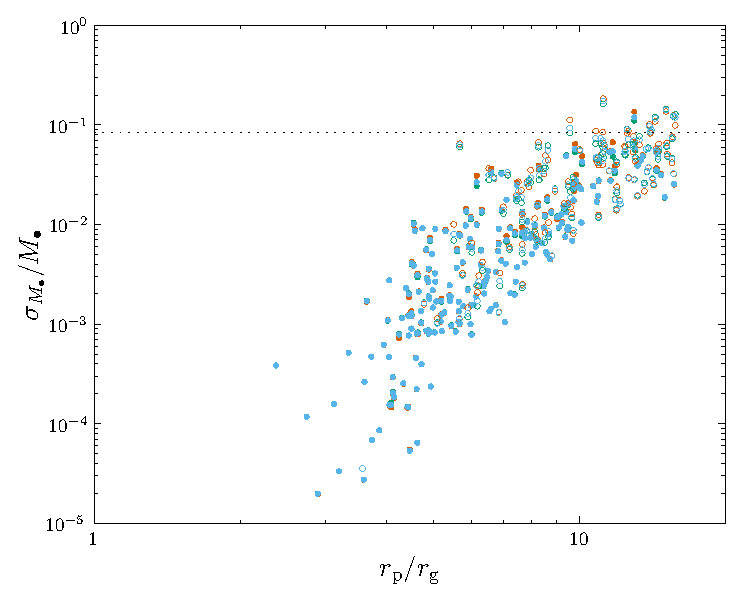
\includegraphics[width=0.475\textwidth]{./images/Fig_MCMC_sigmas_rp_1}} \quad
\subfigure[MBH mass $M_\bullet$ versus SNR.]{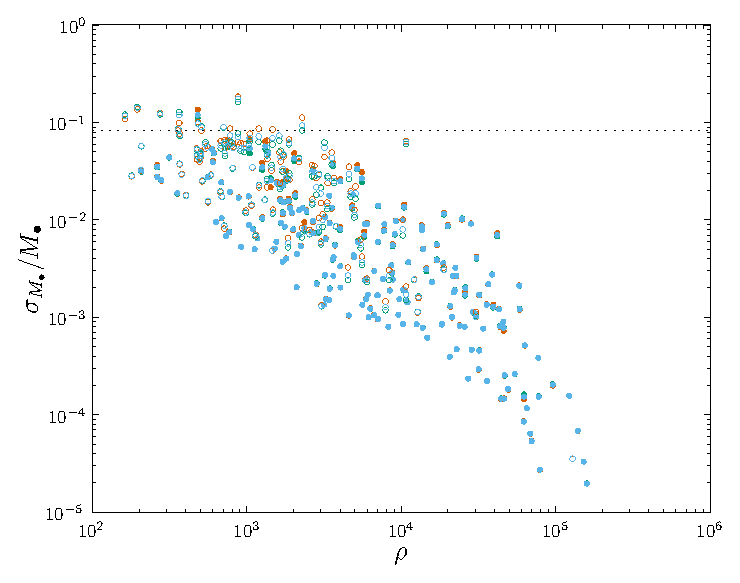
\includegraphics[width=0.485\textwidth]{./images/Fig_MCMC_sigmas_SNR_1}} \\
\subfigure[MBH spin $a_\ast$ versus periapsis.]{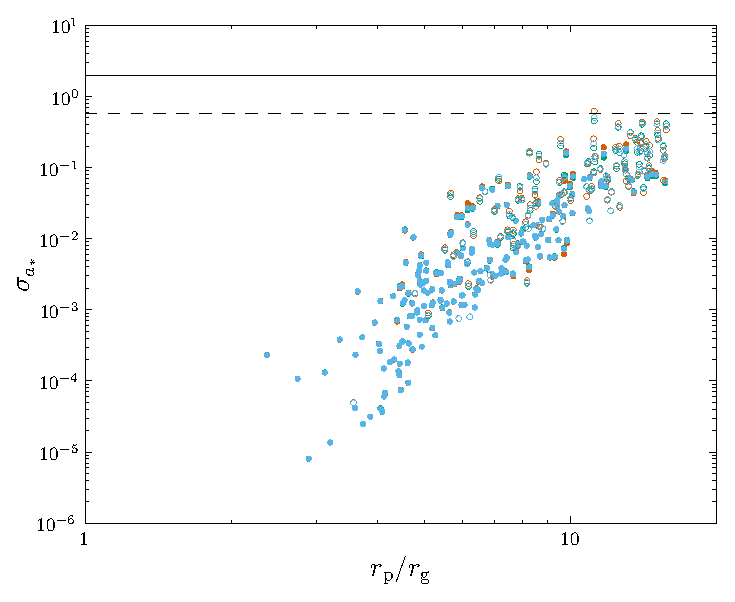
\includegraphics[width=0.475\textwidth]{./images/Fig_MCMC_sigmas_rp_2}} \quad
\subfigure[MBH spin $a_\ast$ versus SNR.]{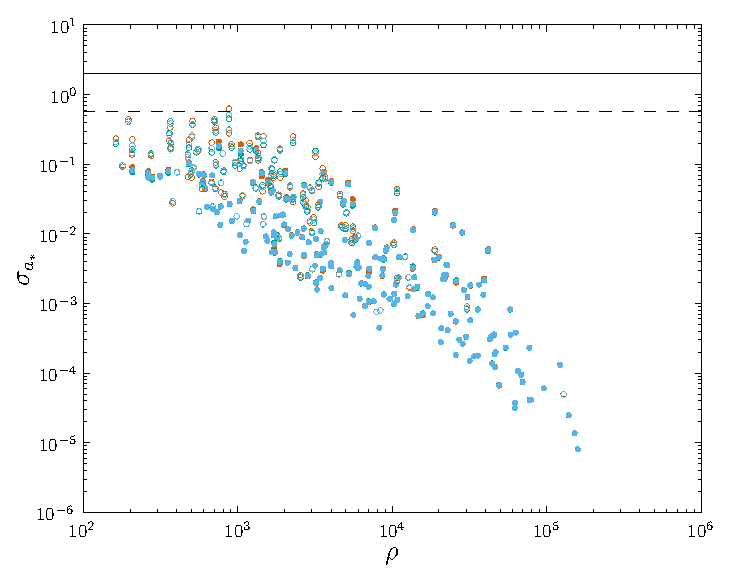
\includegraphics[width=0.485\textwidth]{./images/Fig_MCMC_sigmas_SNR_2}} \\
\subfigure[Orientation angle $\Theta\sub{K}$ versus periapsis.]{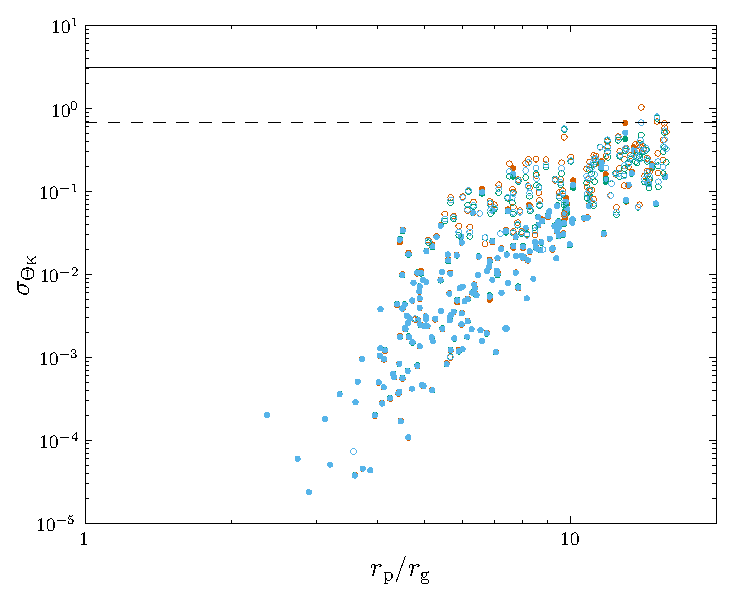
\includegraphics[width=0.475\textwidth]{./images/Fig_MCMC_sigmas_rp_8}} \quad
\subfigure[Orientation angle $\Theta\sub{K}$ versus SNR.]{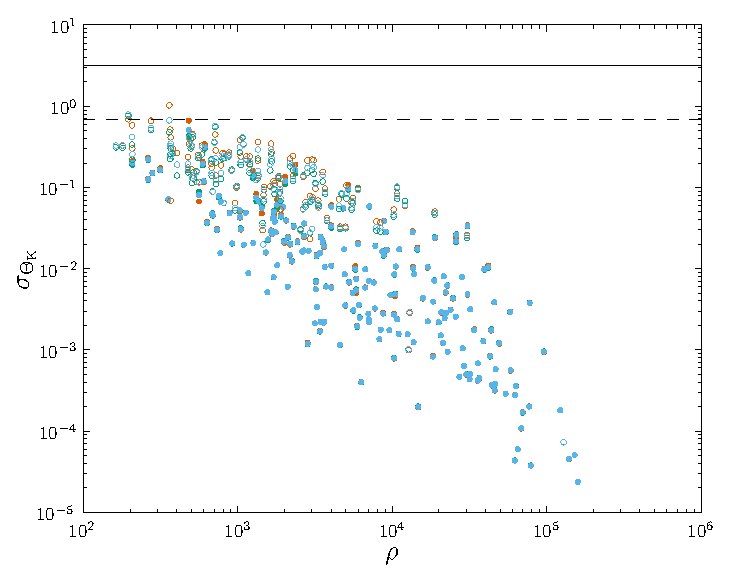
\includegraphics[width=0.485\textwidth]{./images/Fig_MCMC_sigmas_SNR_8}}
\caption{Distribution widths as functions of periapse $r\sub{p}$ and SNR $\rho$. Light blue is used for the standard deviation, red is the scaled $50$-percentile range and green is the scaled $95$-percentile range: all three coincide for a normal distribution. Filled circles are used for converged runs, open circles for those yet to converge. The dotted line indicates the current uncertainty for $M_\bullet$; the dashed lines the standard deviation for an uninformative prior, and the solid lines the total prior range.\label{fig:sigmas}}
\end{center}
\end{figure}
\begin{figure}[!htp]
\setcounter{subfigure}{6}
\begin{center}
\subfigure[Orientation angle $\Phi\sub{K}$ versus periapsis.]{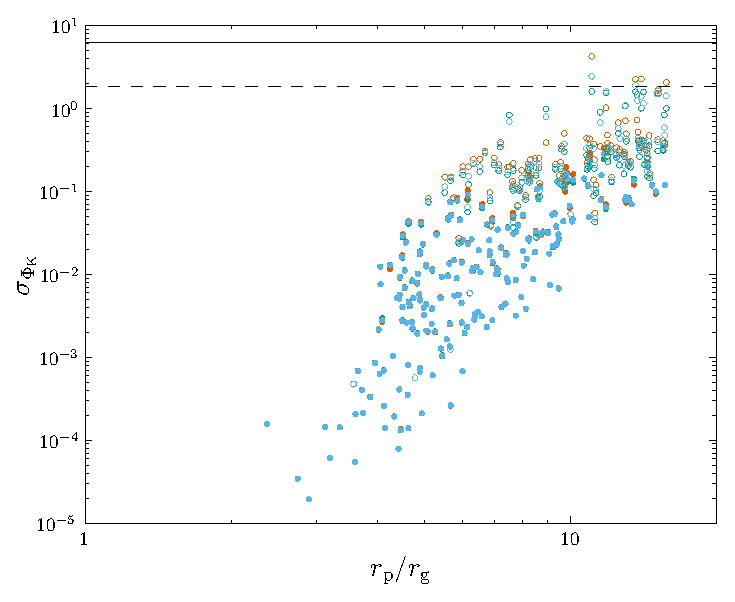
\includegraphics[width=0.475\textwidth]{./images/Fig_MCMC_sigmas_rp_9}} \quad
\subfigure[Orientation angle $\Phi\sub{K}$ versus SNR.]{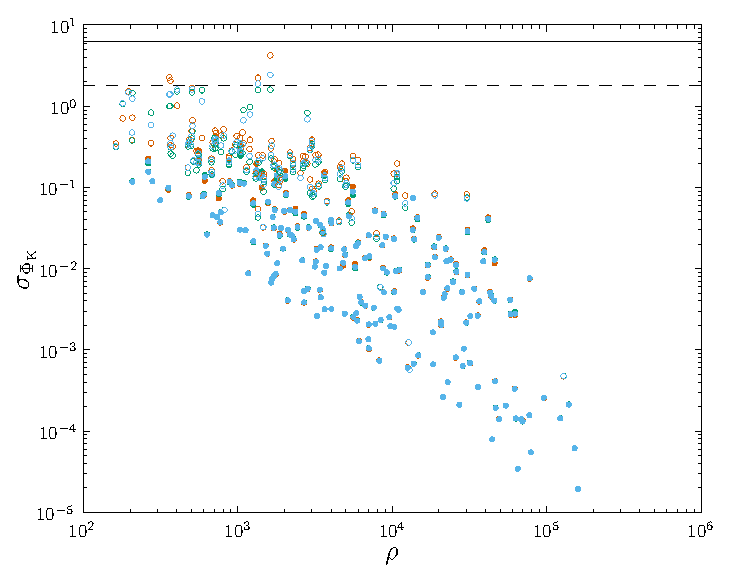
\includegraphics[width=0.485\textwidth]{./images/Fig_MCMC_sigmas_SNR_9}} \\
\subfigure[Scaled distance $\zeta$ versus periapsis.]{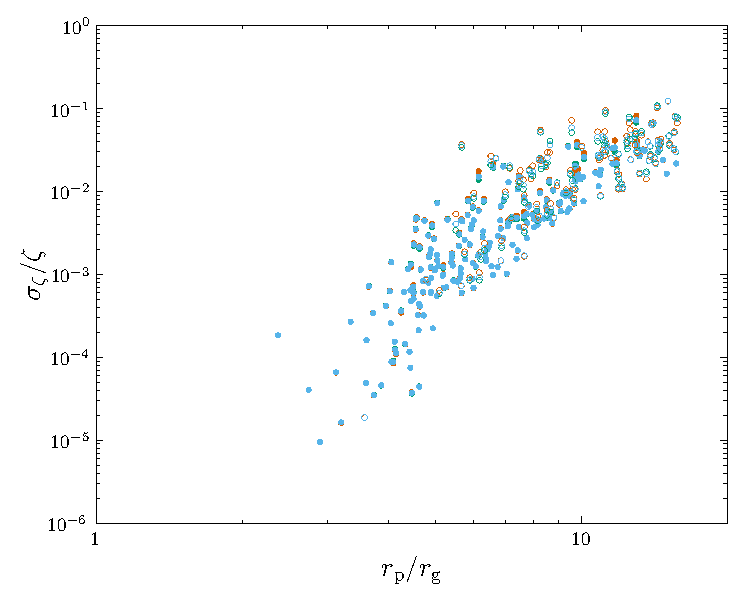
\includegraphics[width=0.475\textwidth]{./images/Fig_MCMC_sigmas_rp_10}} \quad
\subfigure[Scaled distance $\zeta$ versus SNR.]{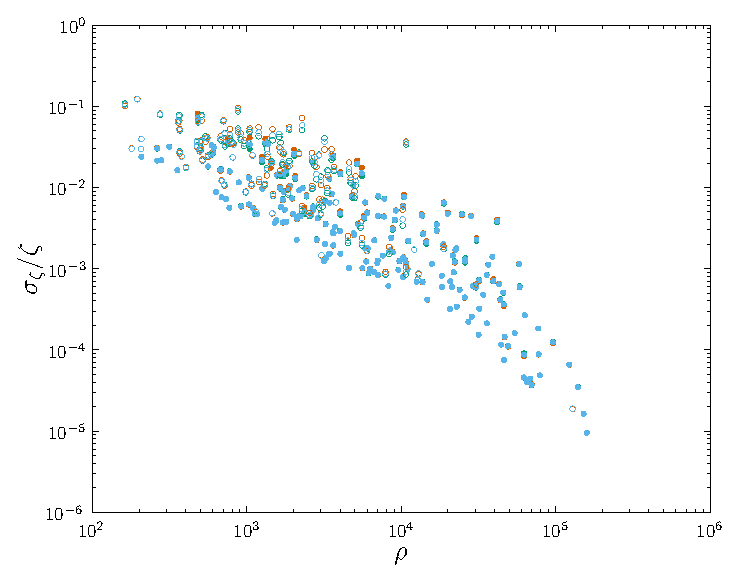
\includegraphics[width=0.485\textwidth]{./images/Fig_MCMC_sigmas_SNR_10}} \\
\subfigure[Angular momentum $L_\infty$ versus periapsis.]{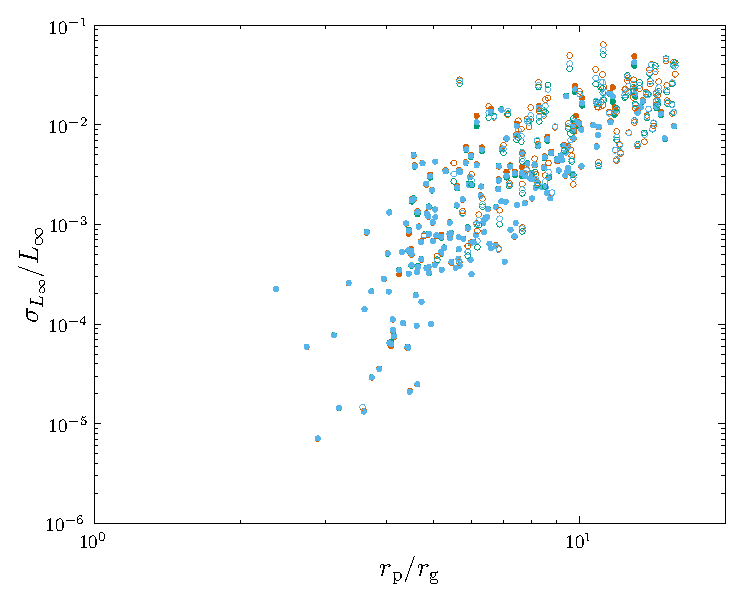
\includegraphics[width=0.475\textwidth]{./images/Fig_MCMC_sigmas_rp_3}} \quad
\subfigure[Angular momentum $L_\infty$ versus SNR.]{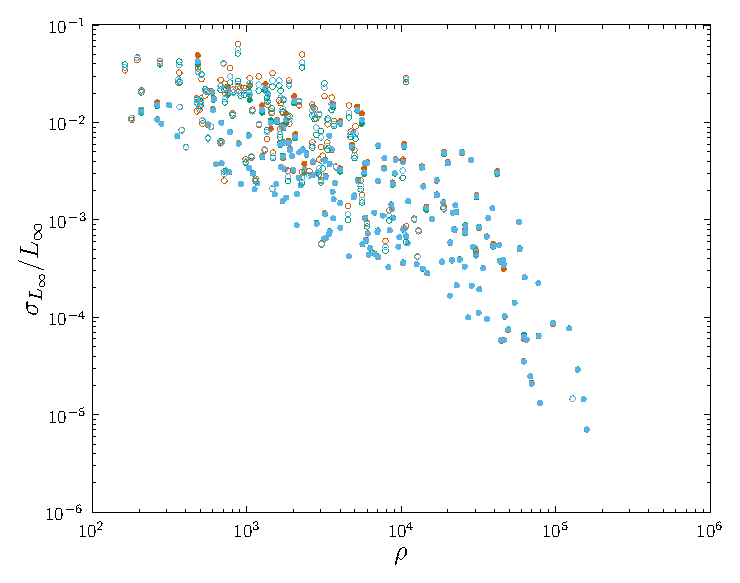
\includegraphics[width=0.485\textwidth]{./images/Fig_MCMC_sigmas_SNR_3}} \\
\contcaption{Distribution widths as functions of periapse $r\sub{p}$ and SNR $\rho$. Light blue is used for the standard deviation, red is the scaled $50$-percentile range and green is the scaled $95$-percentile range: all three coincide for a normal distribution. Filled circles are used for converged runs, open circles for those yet to converge. The dotted line indicates the current uncertainty for $M_\bullet$; the dashed lines the standard deviation for an uninformative prior, and the solid lines the total prior range.}
\end{center}
\end{figure}
\begin{figure}[!htp]
\setcounter{subfigure}{12}
\begin{center}
\subfigure[Orbital inclination $\iota$ versus periapsis.]{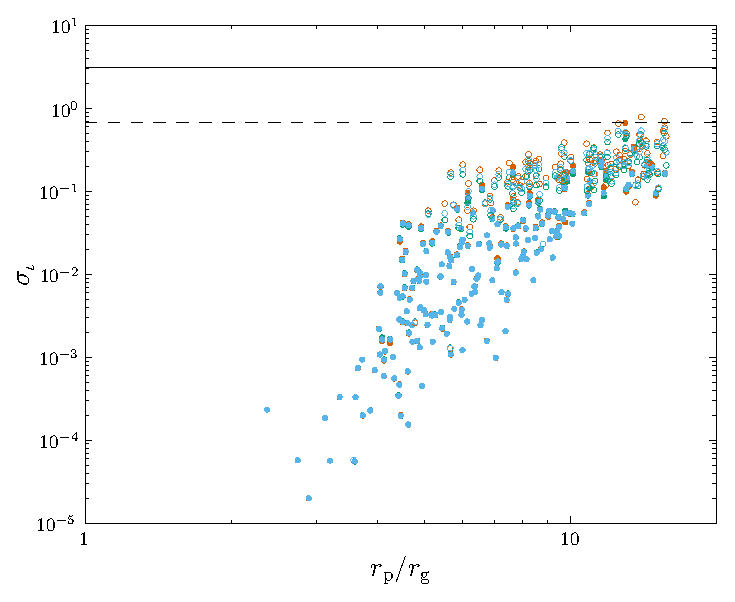
\includegraphics[width=0.475\textwidth]{./images/Fig_MCMC_sigmas_rp_4}} \quad
\subfigure[Orbital inclination $\iota$ versus SNR.]{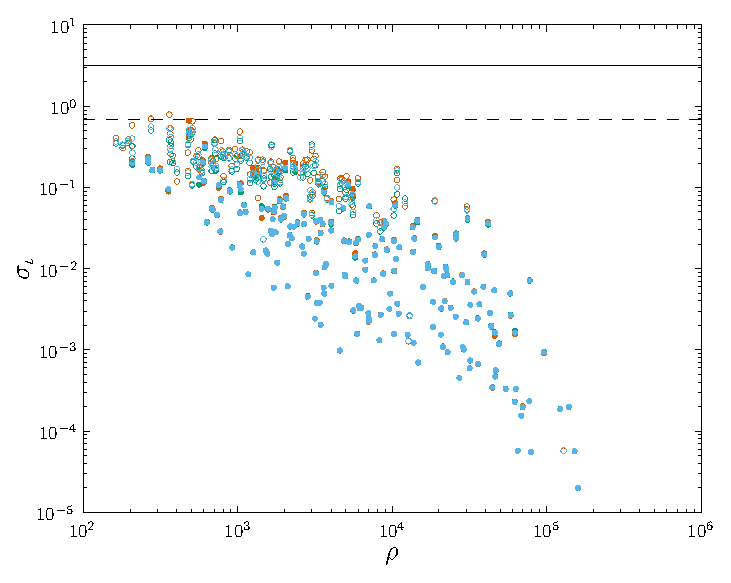
\includegraphics[width=0.485\textwidth]{./images/Fig_MCMC_sigmas_SNR_4}} \\
\subfigure[Periapse azimuthal phase $\phi\sub{p}$ versus periapsis.]{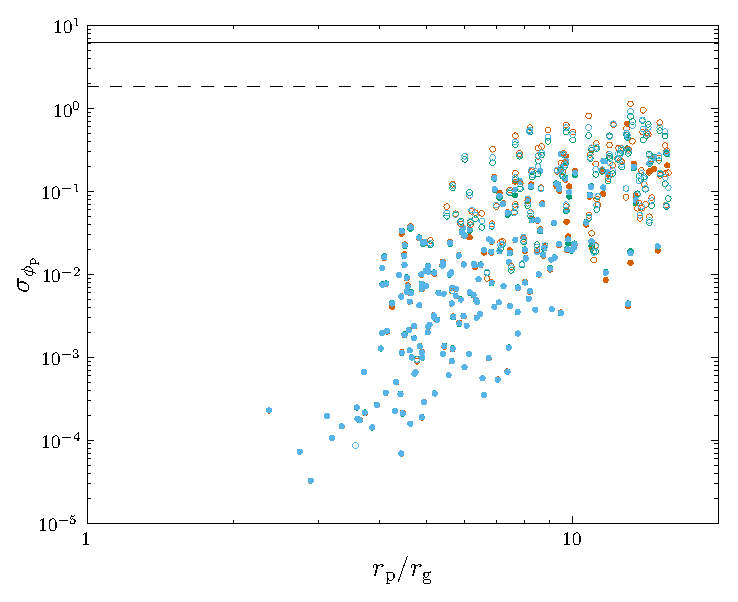
\includegraphics[width=0.475\textwidth]{./images/Fig_MCMC_sigmas_rp_7}} \quad
\subfigure[Periapse azimuthal phase $\phi\sub{p}$ versus SNR.]{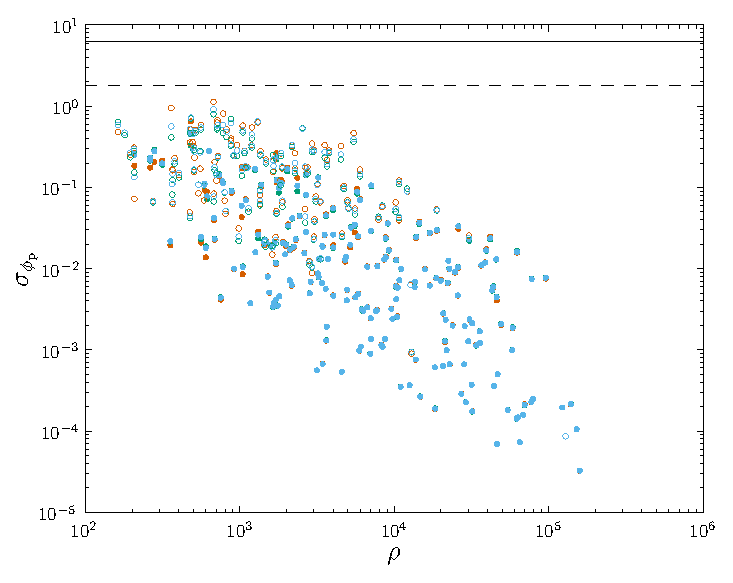
\includegraphics[width=0.485\textwidth]{./images/Fig_MCMC_sigmas_SNR_7}} \\
\subfigure[Periapse polar phase $\chi\sub{p}$ versus periapsis.]{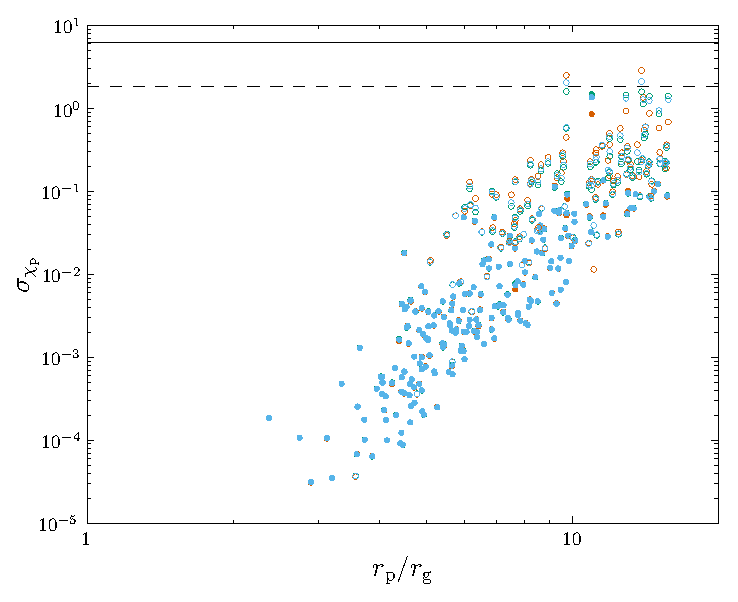
\includegraphics[width=0.475\textwidth]{./images/Fig_MCMC_sigmas_rp_5}} \quad
\subfigure[Periapse polar phase $\chi\sub{p}$ versus SNR.]{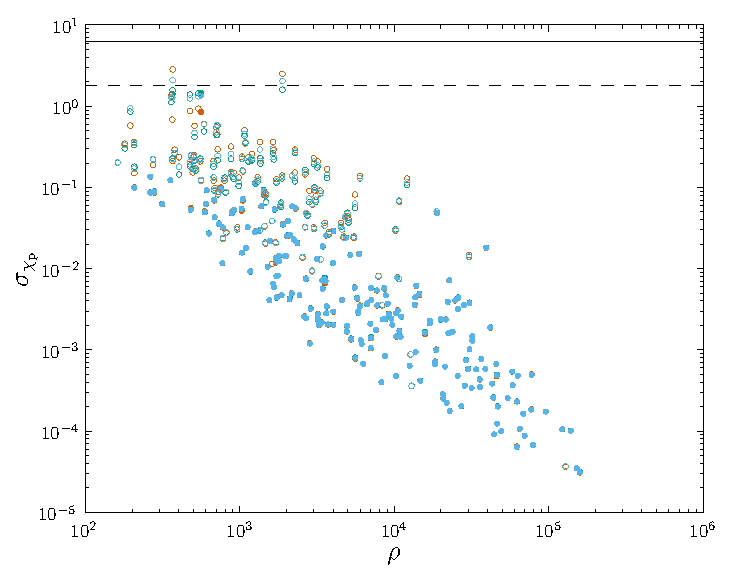
\includegraphics[width=0.485\textwidth]{./images/Fig_MCMC_sigmas_SNR_5}} \\
\contcaption{Distribution widths as functions of periapse $r\sub{p}$ and SNR $\rho$. Light blue is used for the standard deviation, red is the scaled $50$-percentile range and green is the scaled $95$-percentile range: all three coincide for a normal distribution. Filled circles are used for converged runs, open circles for those yet to converge. The dotted line indicates the current uncertainty for $M_\bullet$; the dashed lines the standard deviation for an uninformative prior, and the solid lines the total prior range.}
\end{center}
\end{figure}
\begin{figure}[!htp]
\setcounter{subfigure}{18}
\begin{center}
\subfigure[Periapse time $t\sub{p}$ versus periapsis.]{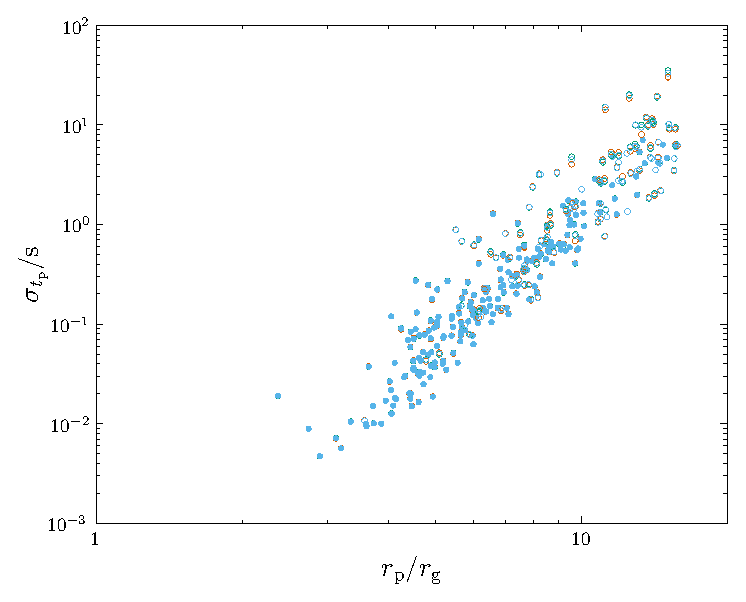
\includegraphics[width=0.475\textwidth]{./images/Fig_MCMC_sigmas_rp_6}} \quad
\subfigure[Periapse time $t\sub{p}$ versus SNR.]{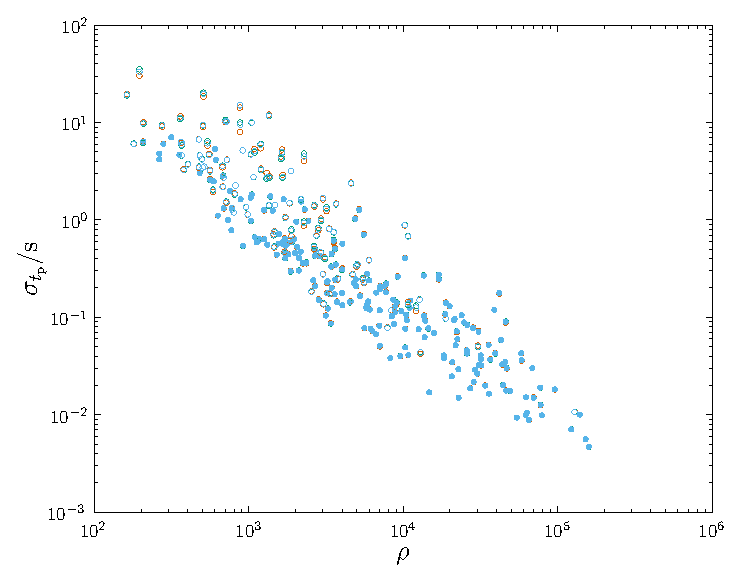
\includegraphics[width=0.485\textwidth]{./images/Fig_MCMC_sigmas_SNR_6}} \\
\contcaption{Distribution widths as functions of periapsis $r\sub{p}$ and SNR $\rho$. Light blue is used for the standard deviation, red is the scaled $50$-percentile range and green is the scaled $95$-percentile range: all three coincide for a normal distribution. Filled circles are used for converged runs, open circles for those yet to converge. The dotted line indicates the current uncertainty for $M_\bullet$; the dashed lines the standard deviation for an uninformative prior, and the solid line the total prior range.}
\end{center}
\setcounter{subfigure}{0}
\end{figure}
For guidance, the dotted line corresponds to the current measurement uncertainty for $M_\bullet$; the dashed lines are from uniform priors for $a_\ast$, $\Phi\sub{K}$, $\phi\sub{p}$, $\chi\sub{p}$, $\cos\Theta\sub{K}$ and $\cos\iota$, and, for completeness, the solid line indicates the total prior range. We have no expectations for the width of the MBH mass distribution with respect to the current value; however, we would expect that the recovered distributions for the other parameters are narrower than for the case of complete ignorance. This may not be the case if the distribution is multimodal: in this event using the width is an inadequate description of the distribution. Only a few unconverged runs exceed these limits, and some appear to be multimodal.

The widths show a trend of decreasing with decreasing periapsis or increasing SNR, but there is a large degree of scatter. There does not appear to be a strong dependence upon any single input parameter, with the exception of the spin. The widths for $\iota$, $\Theta\sub{K}$, $\Phi\sub{K}$, $\phi\sub{p}$ and $\chi\sub{p}$ increase for smaller spin magnitudes. The dependence is shown in \figref{sigmas-spin}.
\begin{figure}[!htp]
\begin{center}
\subfigure[MBH spin $a_\ast$.]{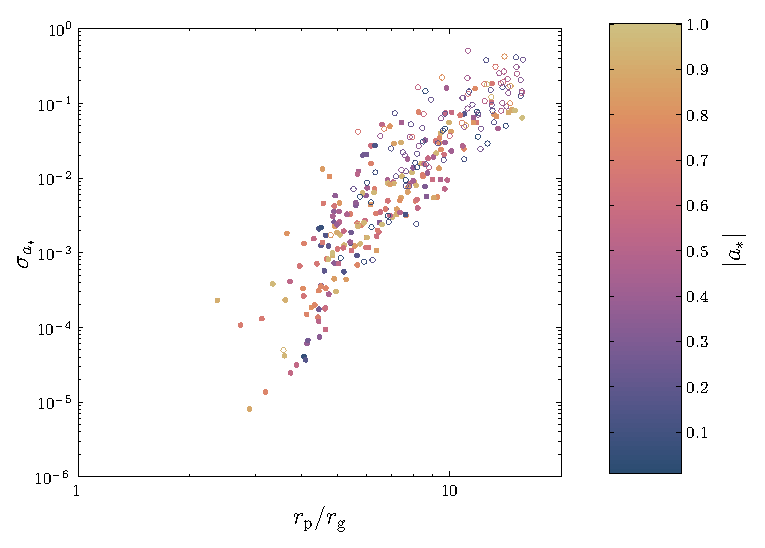
\includegraphics[width=0.48\textwidth]{./images/Fig_MCMC_sigmas_rp_spin_2}} \quad
\subfigure[Orientation angle $\Theta\sub{K}$.]{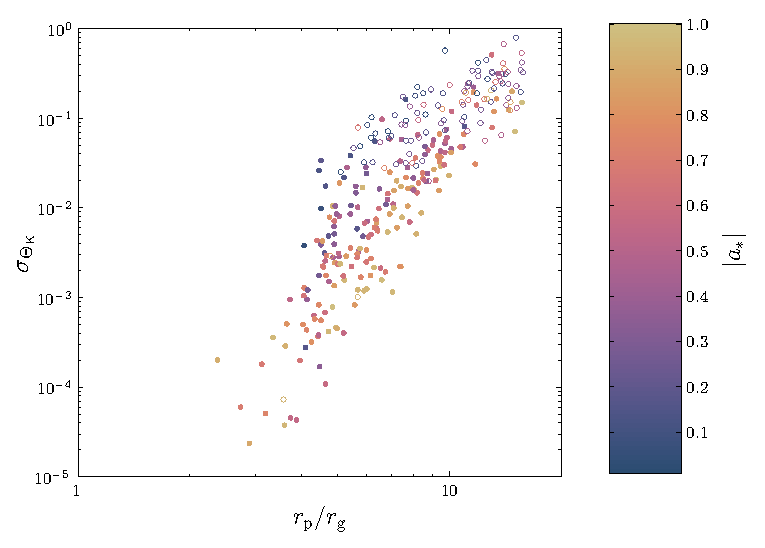
\includegraphics[width=0.48\textwidth]{./images/Fig_MCMC_sigmas_rp_spin_8}} \\
\subfigure[Orientation angle $\Phi\sub{K}$.]{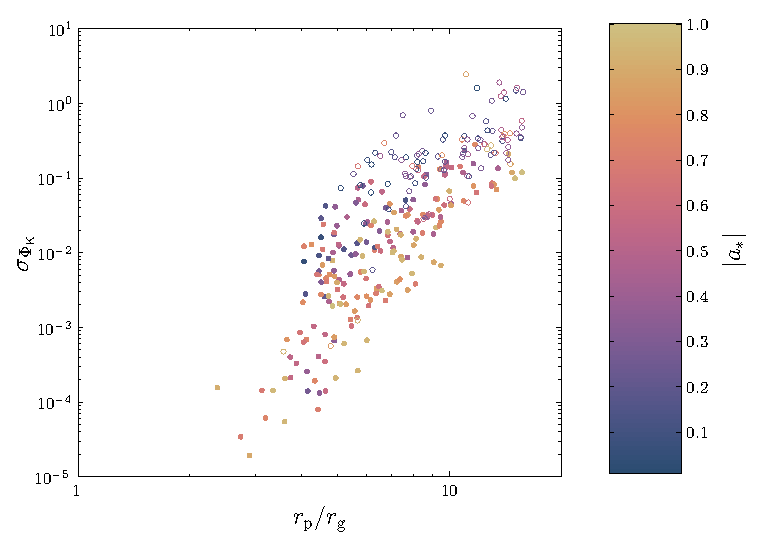
\includegraphics[width=0.48\textwidth]{./images/Fig_MCMC_sigmas_rp_spin_9}} \quad
\subfigure[Orbital inclination $\iota$.]{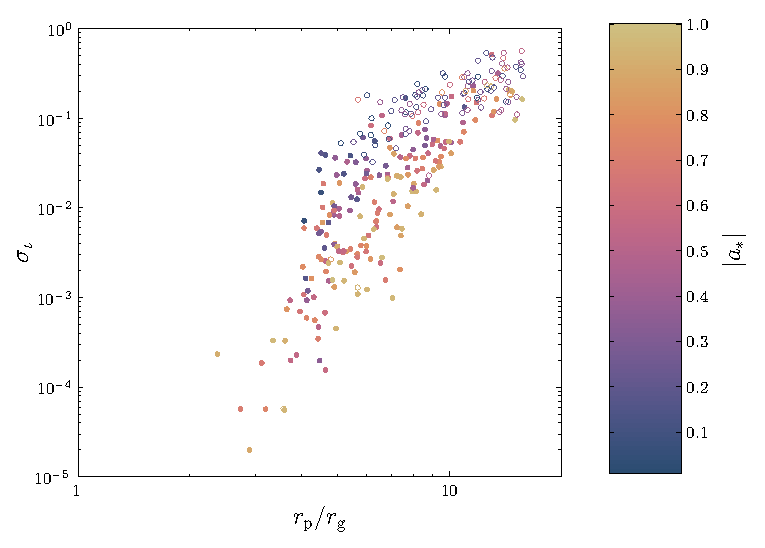
\includegraphics[width=0.48\textwidth]{./images/Fig_MCMC_sigmas_rp_spin_4}} \\
\subfigure[Periapse azimuthal phase $\phi\sub{p}$]{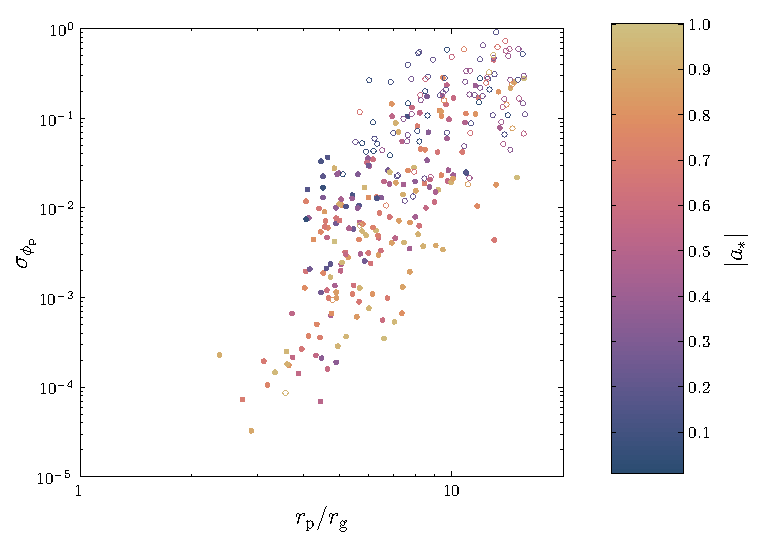
\includegraphics[width=0.48\textwidth]{./images/Fig_MCMC_sigmas_rp_spin_7}} \quad
\subfigure[Periapse polar phase $\chi\sub{p}$.]{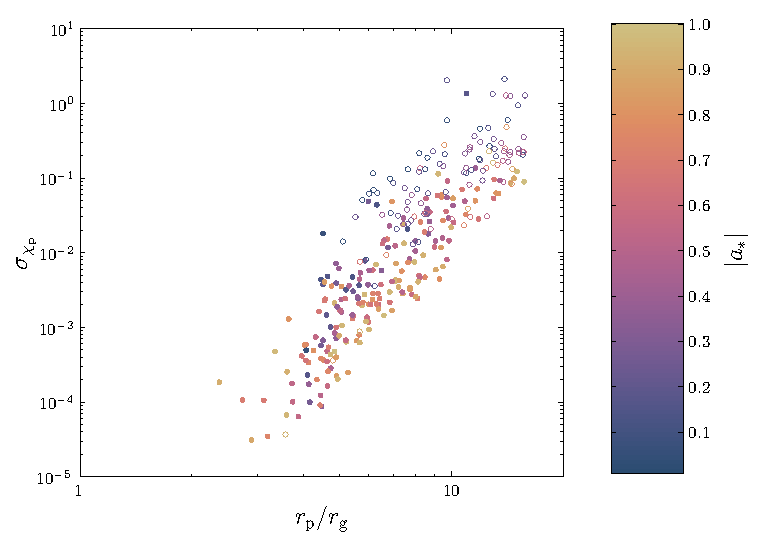
\includegraphics[width=0.48\textwidth]{./images/Fig_MCMC_sigmas_rp_spin_5}}
\caption{Parameter standard deviations versus periapsis $r\sub{p}$, showing dependence (or lack thereof) upon the spin magnitude $|a_\ast|$.\label{fig:sigmas-spin}}
\end{center}
\end{figure}
These parameters are defined with reference to the coordinate system established by the spin axis: for $a_\ast = 0$ we have spherical symmetry and there would be ambiguity in defining them. Therefore, it makes sense that they can be more accurately determined for larger spin magnitudes. The width for $a_\ast$, however, shows no clear correlation.

\subsection{Scientific potential}

Having quantified the precision with which we could infer parameters from an EMRB waveform, we can now consider if it is possible to learn anything new.

Of paramount interest are the MBH mass and spin. The current uncertainty in the mass is $\sigma_{M_\bullet} = 0.36 \times 10^6 M_\odot$ ($\sim 8\%$). There are few runs amongst our data set that are not better than this: it appears that orbits of a $\mu = 10 M_\odot$ CO with periapses $r\sub{p} \lesssim 13 r\sub{g}$ should be able to match our current observational constraints. However, the EMRB is an independent measurement, and so a measurement of comparable precision to the current bound can still be informative. Accuracy of $1\%$ could be possible if $r\sub{p} \lesssim 8 r\sub{g}$.

The spin is less well constrained. To obtain an uncertainty for the magnitude of $0.1$, comparable to that achieved in X-ray measurements of active galactic nuclei, it appears that the periapsis needs to be $r\sub{p} \lesssim 11 r\sub{g}$. For smaller periapses, the uncertainty can be much less, indicating that an EMRB could be an excellent probe. The orientation angles for the spin axis may be constrained to better than $0.1$ for $r\sub{p} \lesssim 11 r\sub{g}$. It may well be possible to learn both the direction and the magnitude of the spin. This could illuminate the MBH's formation.

We have no {\it a priori} knowledge about the CO or its orbit, so anything we learn would be new. However, this is not particularly useful information, unless we observe multiple bursts, and can start to build up statistics for the dynamics of the GC. Using current observations for the distance to the GC, which could be further improved by the mass measurement from the EMRB, it is possible to infer a value for the mass $\mu$ from $\zeta$. This could inform us of the nature of the object (BH, NS or WD) and be a useful consistency check. A small value of $\zeta$, indicating a massive CO, would be unambiguous evidence for the existence of a stellar mass black hole.
%\clearpage

\section{Event rates}\label{sec:Events}

For EMRBs to be a useful astronomical signal we require that the bursts contain sufficient information to improve our knowledge of their source systems and that their event rate is sufficiently high that we could expect to observe them over a mission life time. We have addressed the first: EMRBs can give good constraints on the key parameters describing the Galaxy's MBH. The second concern shall be the addressed here. Previously, the best estimate for the event rate was given by \citet{Hopman2007}; they predicted the event rate for LISA was $\sim 1\units{yr^{-1}}$. We follow a similar approach, but significantly, we improve the calculation of SNR by using NK waveforms.

\subsection{The distribution function}

We wish to calculate the probability there is an encounter between a compact object, on an orbit described by eccentricity $e$ and periapse radius $r\sub{p}$, and the MBH. We begin by following the work of \citet{Bahcall1976, Bahcall1977} and assuming the distribution function (DF) $f$ within the galactic core is only a function of the orbital energy \citep{Shapiro1978}. The energy per unit mass of the orbit is
\begin{equation}
\mathcal{E} = \frac{v^2}{2} - \frac{GM_\bullet}{r},
\end{equation}
where $v$ is orbital velocity. The number of stars is
\begin{equation}
N = \int \dd^3r \int \dd^3v f(\mathcal{E}).
\end{equation}
Close to the centre of the Galactic core, dynamics are dominated by the influence of the MBH as it is significantly more massive than the surrounding stars. Its radius of influence is \citep{Frank1976}
\begin{equation}
r\sub{c} = \frac{GM_\bullet}{\sigma^2},
\label{eq:r_c}
\end{equation}
where $\sigma^2$ is the line-of-sight velocity dispersion. We assume the mass of stars enclosed within $r\sub{c}$ is greater than the $M_\bullet$, which is much greater than the mass of a typical star $M_\star$ \citep{Bahcall1976}. We define a reference number density $n_\star$ from the enclosed mass $m_\ast(r)$ such that
\begin{equation}
m_\star(r\sub{c}) = \frac{4\pi r\sub{c}^3}{3}n_\star M_\star.
\end{equation}
Within the core, the DF can be calculated using the approximation of Fokker-Planck formalism \citep[section 7.4]{Binney2008}. The population of bound stars is evolved numerically until a steady state is reached: the unbound stars form a reservoir with an assumed Maxwellian distribution. Denoting a species of star by its mass $M$,
\begin{equation}
f_M(\mathcal{E}) = \frac{C_M n_\star}{(2\pi\sigma_M^2)^{3/2}} \exp\left(-\frac{\mathcal{E}}{\sigma_M^2}\right),\quad\mathcal{E} > 0,
\label{eq:Unbound_DF}
\end{equation}
where $C_M$ is a normalisation constant.\footnote{$C_M$ determines the population ratios of species $M$ far from the black hole \citep{Alexander2009}.} If different stellar species are in equipartition, as assumed by \citet{Bahcall1976, Bahcall1977}, we expect
\begin{equation}
M \sigma_M^2 = M_\star \sigma_\star^2.
\end{equation}
However, if the unbound stellar population has reached equilibrium by violent relaxation, all mass groups are expected to have similar dispersions:
\begin{equation}
\sigma_M = \sigma_\star = \sigma,
\end{equation}
and we have equipartition of energy per unit mass \citep{Lynden-Bell1967}. This is assumed here following \citet{Alexander2009} and \citet{O'Leary2009}. The steady-state DF is largely insensitive to this choice \citep{Bahcall1977, Alexander2009}.

For bound orbits, the DF can be approximated as a power law \citep{Peebles1972}
\begin{equation}
f_M(\mathcal{E}) = \frac{k_M n_\star}{(2\pi\sigma^2)^{3/2}}\left(-\frac{\mathcal{E}}{\sigma^2}\right)^{p_M},\quad\mathcal{E} < 0.
\label{eq:Bound_DF}
\end{equation}
The exponent $p_M$ varies depending upon the mass of the object, determining mass segregation. For a system with a single mass component $p = 1/4$ \citep{Bahcall1976, Young1977}. The normalisation constant $k_M$ reflects the relative abundances of the different species.\footnote{For a single mass population ($p = 1/4$) $k = 2 C$ gives a fit correct to within a factor of two \citep{Bahcall1976,Keshet2009}, we assume this holds for the dominant species of stars as, although it changes slightly with $p$, variation is small compared to errors introduced by fitting a simple power law \citep{Hopman2006, Alexander2009}.}

These cusp profiles should exist if the system has had sufficient time to become gravitationally relaxed. There is current debate about whether this may be the case, both for the Galactic centre and galaxies in general. This is discussed further in \apref{tauGC}. For concreteness, we assume a cusp has formed. If a cusp has not formed, we expect there to be a shallower core profile, with fewer objects passing close to the MBH. Our results are therefore an upper bound on possible event rates \citep{Merritt2010a,Gualandris2012}. 

\subsection{Model parameters}\label{sec:GC-Param}

We use the Fokker-Planck model of \citet{Hopman2006, Hopman2006a, Alexander2009}. This includes four stellar species: main sequence (MS) stars, white dwarfs (WDs), neutron stars (NSs), and black holes (BHs). Their properties are summarised in \tabref{HA}. The behaviour of the Fokker-Planck model has been verified by $N$-body simulations \citep{Baumgardt2004,Preto2010}.
\begin{table}
 \centering
  \begin{tabular}{l D{.}{.}{2.1} D{.}{.}{1.3} D{.}{.}{1.1} D{.}{.}{1.3}}
  \toprule
   Star & \multicolumn{1}{c}{$M/M_\odot$} & \multicolumn{1}{c}{$C_M/C_\star$} & \multicolumn{1}{c}{$p_M$} & \multicolumn{1}{c}{$k_M/k_\star$\footnote{\citet*{Toonen2009}}} \\
 \midrule
 MS & 1.0 & 1 & -0.1 & 1 \\
 WD & 0.6 & 0.1 & -0.1 & 0.09 \\
 NS & 1.4 & 0.01 & 0.0 & 0.01  \\
 BH & 10 & 0.001 & 0.5 & 0.008 \\
\bottomrule
\end{tabular}
\caption{Stellar model parameters for the galactic centre using the results of \citet{Alexander2009} We use the main sequence star as our reference. The number fractions for unbound stars are estimates corresponding to a model of continuous star formation \citep{Alexander2005}; \citet{O'Leary2009} arrive at the same proportions.\label{tab:HA}}
\end{table}
The steeper power law for black holes means they segregate about the MBH\footnote{Extrapolating, they would dominate in place of MS stars for radii $r < 10^{-4}r\sub{c}$.}

Binaries may form in the galactic centre, encouraged by its high stellar density \citep{O'Leary2009}. However the binary fraction is still expected to be small \citep{Hopman2009}. Binaries are also disrupted by the MBH for periapses smaller than
\begin{equation}
r\sub{B}  \simeq \left(\frac{M_\bullet}{M_1 + M_2}\right)^{1/3}a\sub{B},
\end{equation}
where $M_1$ and $M_2$ are the masses of the binary's components, and $a\sub{B}$ is the binary's semi-major axis, cf.\ \eqnref{Tidal} below. Thus, we ignore the possible presence of binaries.

We assume $M_\bullet = (4.31 \pm 0.36) \times 10^6 M_\odot$ \citep{Gillessen2009} and $\sigma = (103 \pm 20)\units{km\,s^{-1}}$ \citep{Tremaine2002}. This gives a core radius of $r\sub{c} = (1.7 \pm 0.7)\units{pc}$. Using the results of \citet{Ghez2008} we would expect the total mass of stars core to be $m_\star(r\sub{c}) = 6.4 \times 10^6 M_\odot$, which is within $5\%$ of the value obtained similarly from \citet{Genzel2003}. This gives a reference stellar density of $n_\star = 2.8 \times 10^5\units{pc^{-3}}$.

\subsection{Parametrising in terms of eccentricity \& periapsis}

We characterise orbits by their eccentricity $e$ and periapse radius $r\sub{p}$. The latter, unlike the semimajor axis, is always well defined regardless of eccentricity. For Keplerian orbits, the energy $\mathcal{E}$ and angular momentum $\mathcal{J}$ per unit mass are entirely characterised by these parameters
\begin{align}
\label{eq:Energy_ecc}
\mathcal{E} = {} & -\frac{GM_\bullet(1 - e)}{2r\sub{p}}; \quad \mathcal{J}^2 = GM_\bullet(1 + e)r\sub{p}.
\end{align}
The DF is defined per element of phase space: it is necessary to change variables from position and velocity to eccentricity and periapsis. We decompose the velocity into three orthogonal components: radial $v_r$, azimuthal $v_\phi$ and polar $v_\theta$. We assume the galactic core is spherically symmetric \citep{Genzel2003, Schodel2007}, therefore we are only interested in the combination
\begin{equation}
v_\perp^2 = v_\phi^2 + v_\theta^2 = v^2 - v_r^2.
\end{equation}
Under this change of variables
\begin{equation}
\dd^3v = \dd v_r \dd v_\phi \dd v_\theta \rightarrow 2\pi v_\perp \,\dd v_r \,\dd v_\perp.
\end{equation}
The specific energy and angular momentum are given by
\begin{align}
\mathcal{E} = {} & \frac{v_r^2 + v_\perp^2}{2} - \frac{GM_\bullet}{r}; \quad \mathcal{J}^2 = r^2 v_\perp^2.
\end{align}
Combining these with our earlier expressions in terms of $e$ and $r\sub{p}$,
\begin{align}
v_\perp^2 = {} & \frac{GM_\bullet(1 + e)r\sub{p}}{r^2}, \\*
v_r^2 = {} & GM_\bullet\left[\frac{2}{r} - \frac{(1 - e)}{r\sub{p}} - \frac{(1 + e)r\sub{p}}{r^2}\right].
\end{align}
From the latter we can verify the turning points of an orbit occur at
\begin{equation}
r = r\sub{p}, \: \frac{1+e}{1-e}r\sub{p};
\end{equation}
the periapse is the only turning point for orbits with $e > 1$. Since we now have expressions for $\{v_r, v_\perp\}$ in terms of $\{e, r\sub{p}\}$, we can 
%calculate the Jacobian
%\begin{equation}
%\left|\frac{\partial(v_r, v_\perp)}{\partial(e, r\sub{p})}\right| = \recip{2v_rv_\perp}\frac{e}{r\sub{p}}\left(\frac{GM_\bullet}{r}\right)^2.
%\end{equation}
%Using this, we may
rewrite our velocity element as
\begin{equation}
\dd^3v \rightarrow \frac{\pi e}{v_rr\sub{p}}\left(\frac{GM_\bullet}{r}\right)^2\,\dd e \,\dd r\sub{p}.
\end{equation}
As a consequence of our assumed spherical symmetry, 
%the volume element is
%\begin{equation}
%\dd^3r = 4\pi r^2 \,\dd r.
%\end{equation}
%Thus, 
the phase space volume element can be expressed as
\begin{equation}
\dd^3r\dd^3v \rightarrow \frac{4\pi^2(GM_\bullet)^2e}{v_rr\sub{p}}\,\dd r\,\dd e \,\dd r\sub{p}.
\end{equation}
The number of stars in an element $\dd r\,\dd e\,\dd r\sub{p}$ is
\begin{equation}
n(r, e, r\sub{p}) = \frac{4\pi^2(GM_\bullet)^2e}{v_rr\sub{p}}f(\mathcal{E}).
\end{equation}

From this, we can construct the expected number of stars on orbits defined by $\{e, r\sub{p}\}$. We define this locally, allowing it to vary with position. The number of stars found in a small radius range $\delta r$ with given orbital properties is
\begin{equation}
n(r, e, r\sub{p})\delta r = N(e, r\sub{p}; r)\frac{\delta t}{P(e, r\sub{p})},
\end{equation}
where $N(e, r\sub{p}; r)$ is the total number of stars with orbits given by $\{e, r\sub{p}\}$ defined at $r$, $\delta t$ is the time spent in $\delta r$ and $P(e, r\sub{p})$ is the period of the orbit. We defer the definition of this time for unbound orbits for now. The time spent in the radius range is
\begin{equation}
\delta t = 2\frac{\delta r}{v_r},
\end{equation}
where the factor of $2$ is accounts for inwards and outwards motion. Hence
\begin{align}
N(e, r\sub{p}; r) = {} & \recip{2} v_r P(e, r\sub{p}) n(r, e, r\sub{p}) \nonumber \\
 = {} & \frac{2\pi^2(GM_\bullet)^2 e P(e, r\sub{p})}{r\sub{p}}f(\mathcal{E}).
\end{align}
The right hand side is independent of position, subject to the constraint that the radius is in the allowed range for the orbit $r\sub{p} \leq r \leq (1+e)r\sub{p}/(1-e)$, and so $N(e, r\sub{p}) \equiv N(e, r\sub{p}; r)$. This is a consequence of the DF being dependent only upon a constant of the motion.\footnote{See \citet{Bahcall1976} equation (9) for a similar result.}

If a burst of radiation is emitted each time a star passes through periapse, the event rate for burst emission from orbits with parameters $\{e, r\sub{p}\}$ is given by
\begin{align}
\Gamma(e, r\sub{p}) = {} & \frac{N(e, r\sub{p})}{P(e, r\sub{p})} = \frac{2\pi^2(GM_\bullet)^2 e}{r\sub{p}}f(\mathcal{E}).
\label{eq:Gamma}
\end{align}
The orbital period drops out from the calculation, so we do not have to worry about an appropriate definition for unbound orbits.

%From the event rate we may define a probability of seeing a given number of events subject to the assumption they are uncorrelated: it is given by the Poisson distribution. The probability of there being $r$ events is
%\begin{equation}
%\Pr(r|\Gamma(e, r\sub{p})) = \frac{\Gamma^r\exp(-\Gamma)}{r!}.
%\end{equation}
%The probability of there being a burst from an orbit with periapse $r\sub{p}$ and eccentricity $e$ is hence
%\begin{equation}
%\Pr(r \neq 0|\Gamma(e, r\sub{p})) = 1 - \Pr(r = 0|\Gamma(e, r\sub{p})).
%\end{equation}

%To estimate the expectation of a quantity across all orbits we use
%\begin{equation}
%\left\langle X\right\rangle = \sum\sub{R} \int_0^\infty \dd e \int_0^\infty \dd r\sub{p} X(r;r\sub{p},e)\Pr(r|\Gamma(e, r\sub{p})).
%\end{equation}
%Since the probability decays rapidly for large $r$, we may truncate the sum to give the required level of accuracy,

To generate a representative sample for the orbital parameters $e$ and $r\sub{p}$, we use $\Gamma(e, r\sub{p})\dd e\, \dd r\sub{p}$ as the rate for a Poisson distribution.

\subsection{The inner cut-off}

From \eqnref{Gamma} we see the event rate is highly sensitive to the smallest value of the periapsis. Ultimately the orbits cannot encroach closer to the MBH than its last stable orbit. This depends upon the spin of the MBH, but is of the order of its Schwarzschild radius. Before we reach this point, there are other processes that may intervene to deplete the orbiting stars. Our treatment of these is approximate, but should produce reasonable estimates. We consider three processes: tidal disruption by the MBH; GW inspiral, and collisional disruption. Tidal disruption imposes a definite (albeit approximate) cut-off, while the others use statistical arguments. For these methods, we will need to define a reference time-scale for relaxation which is done in \secref{Relax}, with further details found in \apref{time-scale}.

The calculated inner cut-offs for the four stellar species are shown in \figref{Cuts}.
\begin{figure}[!htp]
\begin{center}
   \subfigure[{Main sequence stars}]{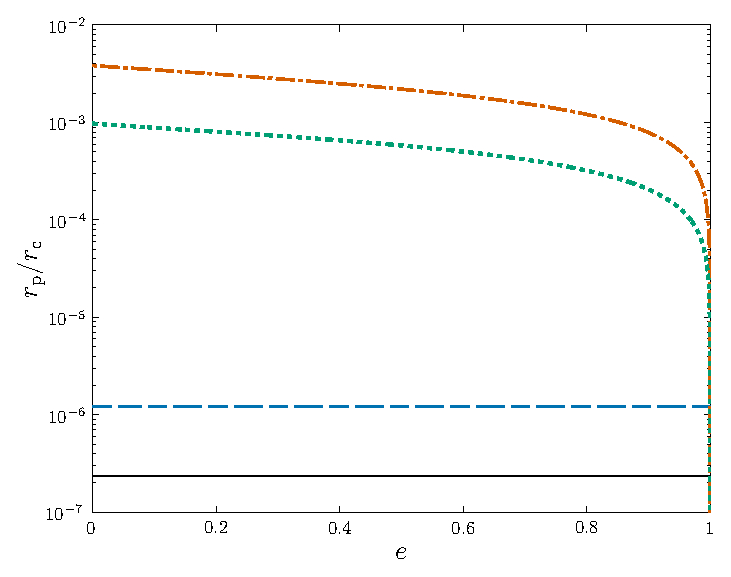
\includegraphics[width=0.4\textwidth]{Fig_Inner_cut_1.eps}} \quad 
   \subfigure[{White dwarfs}]{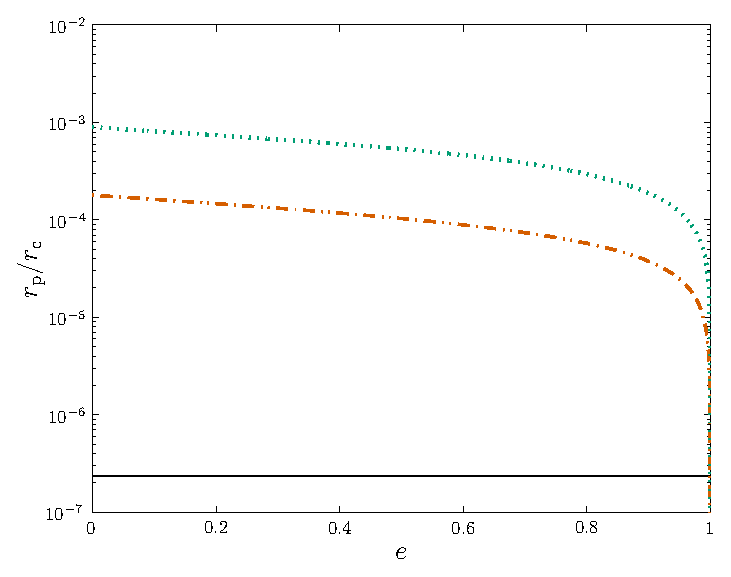
\includegraphics[width=0.4\textwidth]{Fig_Inner_cut_2.eps}} \\
   \subfigure[{Neutron stars}]{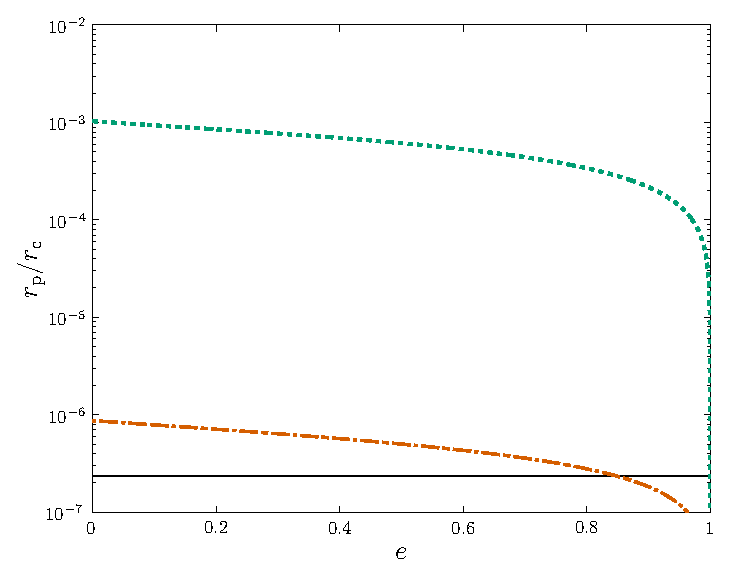
\includegraphics[width=0.4\textwidth]{Fig_Inner_cut_3.eps}} \quad
   \subfigure[{Black holes}]{\includegraphics[width=0.4\textwidth]{Fig_Inner_cut_4.eps}}
\caption{Inner cut-off radii for the Galactic Centre as a function of eccentricity. The solid line is the Schwarzschild radius of the MBH; the dashed line is the tidal radius; the dot-dashed line is the collisional cut-off, and the dotted line is the transition to the GW-dominated inspiral regime.\label{fig:Cuts}}
  \end{center}
\end{figure}

\subsubsection{Tidal disruption}

Tidal forces from the MBH can disrupt stars. This occurs at the tidal radius
\begin{equation}
r\sub{T} \simeq \left(\frac{M_\bullet}{M}\right)^{1/3}R_M
\label{eq:Tidal}
\end{equation}
where $R_M$ is the radius of the star \citep{Hills1975, Rees1988, Kobayashi2004}.\footnote{See \citet{Kesden2012} for a general relativistic treatment.} Any star on an orbit with $r\sub{p} < r\sub{T}$ is disrupted in the course of its orbit. Parametrising orbits by their periapsis allows us to easily determine which stars should be disrupted. We do not include the full effects of the loss cone \citep{Frank1976, Lightman1977, Cohn1978} as these were not incorporated into the Fokker-Planck calculations \citep{Hopman2009}.\footnote{The loss cone is a region in velocity space where orbits are depleted because stars are disrupted more rapidly than they can be replenished by two-body scattering.} The effect of the loss cone should be small, only modifying the DF by a logarithmic term \citep{Lightman1977, Bahcall1977, Cohn1978}. Its effects are diluted by resonant relaxation \citep{Hopman2007,Toonen2009,Merritt2011}. Furthermore, the loss cone could be refilled by the wandering of the MBH because of perturbations from the inhomogeneities in the stellar potential \citep{Sigurdsson1997,Chatterjee2002,Merritt2007}.

Tidal disruption is significant for MS stars since they are least dense: calculated in this way, only MS stars are tidally disrupted outside of the MBH's event horizon \citep{Sigurdsson1997}. The tidal radius defines the cut-off for periapsis of high eccentricity ($e \ga 1$) orbits \citep{Lightman1977}.

\subsubsection{Relaxation time-scale}\label{sec:Relax}

The motion of a star is determined not only by the dominant influence of the central MBH, but also by the other stars. The gravitational potential of the stars may be split into two components: a smooth background representing the average distribution of stars, and statistical fluctuations from random deviations in the stellar distribution. The former only contributes to the stars' orbits: we neglect this since we are more interested in the influence of the MBH. The latter may be approximated as a series of two-body encounters. These lead to scattering, in a manner much like Brownian motion \citep{Bekenstein1992,Maoz1993,Nelson1999}.

The two-body interactions mostly lead to small deflections. Over time, these may accumulate into a significant change in the dynamics. The relaxation time-scale characterises the time taken for this to happen \citep[section 1.2.1]{Binney2008}. It therefore quantifies the time over which an orbit may be repopulated by scattering. There are a variety of definitions for the relaxation time-scale. For a system with a purely Maxwellian distribution, the time-scale has form
\begin{equation}
\tau\sub{R}\super{Max} \simeq \kappa\frac{\sigma^3}{G^2M_\star^2 n_\star\ln\Lambda},
\label{eq:tauMaxwell}
\end{equation}
where the Coulomb logarithm is $\ln\Lambda = \ln(M_\bullet/M_\star)$ \citep{Bahcall1976}, and $\kappa$ is a dimensionless number. In his pioneering work, \citet{Chandrasekhar1941, Chandrasekhar1960} defined the time-scale as the period over which the squared change in energy was equal to the kinetic energy squared, this gives $\kappa = 9/16\sqrt{\pi} \simeq 0.32$. Subsequently, \citet{Chandrasekhar1941a} described relaxation statistically, treating fluctuations in the gravitational field probabilistically; this gives $\kappa = 9/2(2\pi)^{3/2} \simeq 0.29$. \citet{Bahcall1977} define a reference time-scale from their Boltzmann equation with $\kappa = 3/4\sqrt{8\pi} \simeq 0.15$; this is equal to the reference time-scale defined as the reciprocal of the coefficient of dynamical friction by \citet{Chandrasekhar1943a, Chandrasekhar1943}. \citet{Spitzer1958} define a reference time-scale from the gravitational Boltzmann equation of \citet{Spitzer1951} where $\kappa = \sqrt{2}/\pi \simeq 0.45$. Following \citet{Spitzer1971}, \citet[section 7.4.5]{Binney2008} estimate the time-scale from the velocity diffusion coefficient of the Fokker-Planck equation yielding $\kappa \simeq 0.34$.

All these approaches yield consistent values, suggesting, as a first approximation, any is valid. We follow the classic treatment of \citet[chapter 2]{Chandrasekhar1960} which is transparent in its assumptions, adapting from a Maxwellian distribution of velocities to one derived from the DFs \eqnref{Unbound_DF} and \eqnref{Bound_DF}. This makes the model self-consistent. Since there is uncertainty in the astrophysical parameters, we will not be concerned by small discrepancies in the numerical prefactor that result from the simplifying approximations of this approach. Whilst we are only making a minor change to the derivation of the relaxation time-scale, the calculations become much more involved, we confine this to \apref{time-scale}, along with a discussion of the shortcomings. An average time-scale for the entire system $\overline{\tau\sub{R}}$ is defined in \eqnref{system-relax}, and an average for an orbit $\left\langle\tau\sub{R}\right\rangle$ is defined in \eqnref{orbital-relax}.

Two-body interactions lead to diffusion in both energy and angular momentum. When considering a single (bound) orbit, over a relaxation time-scale the energy changes by order of itself while the angular momentum changes by the angular momentum of a circular orbit with that energy $\mathcal{J}\sub{circ}(\mathcal{E})$ \citep{Lightman1977, Rauch1996, Hopman2005, Madigan2011}:\footnote{$\mathcal{J}\sub{circ}(\mathcal{E})$ is the maximum value for orbits of that energy.}
\begin{equation}
\left(\frac{\Delta\mathcal{E}}{\mathcal{E}}\right)^{2} \approx \left[\frac{\Delta \mathcal{J}}{\mathcal{J}\sub{circ}(\mathcal{E})}\right]^{2} \approx \frac{t}{\tau\sub{R}}.
\label{eq:diffuse-relax}
\end{equation}
We may define another angular momentum relaxation time-scale as the time taken for the angular momentum to change by order of itself \citep{Merritt2011}
\begin{align}
\tau_\mathcal{J} = {} & \left[\frac{\mathcal{J}}{\mathcal{J}\sub{circ}(\mathcal{E})}\right]^2\tau\sub{R} = \left(1 - e^2\right) \tau\sub{R}.
\label{eq:J-time}
\end{align}
This can be much shorter than the energy relaxation time-scale: diffusion in angular momentum can proceed more rapidly than diffusion in energy.

\subsubsection{Gravitational wave inspiral}\label{sec:GW-in}

Stars orbiting the MBH continually emit gravitational radiation; this carries away energy and angular momentum, causing the stars to inspiral. Using the analysis of \citet{Peters1963} and \citet{Peters1964} for Keplerian binaries, it is possible to define a characteristic inspiral time-scale from the rate of change of energy. For consistency with the relaxation time-scale, we define this as \citep{MiraldaEscude2000, Merritt2011}
\begin{equation}
\tau\sub{GW} \simeq \mathcal{E}\left\langle\diff{\mathcal{E}}{t}\right\rangle^{-1},
\label{eq:tGW-def}
\end{equation}
where the term in angular brackets is the orbit-averaged rate of energy radiation. Using \eqnref{Energy_ecc} and equation (16) of \citet{Peters1963},
\begin{align}
\tau\sub{GW} \simeq {} & \frac{5}{64}\frac{c^5r\sub{p}^4}{G^3MM_\bullet\left(M + M_\bullet\right)}\frac{(1+e)^{7/2}}{(1-e)^{1/2}} \nonumber \\*
 {} & \times {} \left(1+\frac{73}{24}e^2 + \frac{37}{96}e^4\right)^{-1} \\
 \approx {} & \frac{5}{64}\frac{c^5r\sub{p}^4}{G^3MM_\bullet^2}\frac{(1+e)^{7/2}}{(1-e)^{1/2}}\left(1+\frac{73}{24}e^2 + \frac{37}{96}e^4\right)^{-1}.
\end{align}
The characteristic time-scale is a better measure of the depletion of an orbit than the total inspiral time as it only depends upon the parameters of that orbit, and not its future evolution.

The time-scale associated with changes in angular momentum is \citep{Peters1964}
\begin{align}
\tau_{\mathrm{GW},\, \mathcal{J}} \simeq {} & \mathcal{J}\left\langle\diff{\mathcal{J}}{t}\right\rangle^{-1} \\
 \simeq {} & \frac{5}{32}\frac{c^5r\sub{p}^4}{G^3MM_\bullet\left(M + M_\bullet\right)}\frac{(1+e)^{5/2}}{(1-e)^{3/2}}\left(1+\frac{7}{8}e^2\right)^{-1} \\
 \approx {} & \frac{5}{32}\frac{c^5r\sub{p}^4}{G^3MM_\bullet^2}\frac{(1+e)^{5/2}}{(1-e)^{3/2}}\left(1+\frac{7}{8}e^2\right)^{-1}.
\end{align}
This is always greater than the energy time-scale; hence, we only consider changes in energy from GW emission as important for evolution of the system \citep{Hopman2005}.

Unbound stars only undergo a single periapse passage and only radiate one burst of radiation; we therefore neglect any evolution in their orbital parameters.\footnote{Changes are only important for very high eccentricity orbits (\apref{Unbound}). These are very high energy, and exponentially suppressed because of the Boltzmann factor in \eqnref{Unbound_DF}.}

The $(1-e)^{-1/2}$ dependence of $\tau\sub{GW}$ for bound orbits connects the two regimes. The rate of change of energy goes to zero as a consequence of assumping the orbital parameters do not change over the course of an orbit. It is a valid approximation since the large mass-ratio ensures a slow evolution of the system (\apref{Unbound}).

When comparing with the relaxation time-scale we are comparing rates of change, with the shorter time-scale highlighting the more rapid process that dominates the evolution \citep{Amaro-Seoane2007}. We therefore compare $\tau\sub{GW}$ with the orbital relaxation time-scale $\tau_\mathcal{J}$ \citep{Merritt2011}. Orbits with $\tau\sub{GW} < \tau_\mathcal{J}$ become depleted by GW emission faster than they are replenished by scattering. The cusp does not extend to these orbits. Yet, these orbits are not totally depopulated as an object may pass through during its inspiral from greater periapse and eccentricity. The net effect is the distributions of MS stars, WDs and NSs at high eccentricities are relatively unchanged from their cusp states, but the BH population is significantly depleted.

\subsubsection{Collisions}\label{sec:Collision}

As a consequence of the high densities in the galactic core, stars may undergo a large number of close encounters with other stars \citep{Cohn1978}. These may lead to their destruction. MS stars, WDs, and NSs may be pulled apart by tidal forces if they stray too close to a a more massive object. As MS stars are diffuse, they would not tidally disrupt another star \citep{Murphy1991,Freitag2005}. Close encounters would result in some mass transfer; the cumulative effect of $20$--$30$ grazing collisions could destroy a MS star \citep{Freitag2006}. The number of collisions a star undergoes in a time interval $\delta t$ is
\begin{equation}
\delta K = n(r) A v(r,e,r\sub{p})\delta t,
\end{equation}
where $A$ is the collisional cross-sectional area. For tidal disruption, where the encounter is with a collapsed object (WD, NS or BH), we set $A = \pi r_{\mathrm{T},\,{M'}}^2$, where $r_{\mathrm{T},\,{M'}}$ is the appropriate tidal radius: like \eqnref{Tidal} but with $M_\bullet$ replaced with the mass of the collapsed object $M'$. For collisions between MS stars, the cross-sectional area is simply the geometric $A = \pi R_\star^2$.\footnote{Here we assume the relative velocity of the colliding stars is much greater than the escape velocity of the star so we may neglect the effects of gravitational focusing.}

For circular orbits we can find the radius at which collisions lead to disruptions by setting $\delta K = 1$ for tidal disruption or $\delta K = 20$ for grazing collisions, and $\delta t = \overline{\tau_\mathrm{R,\,M}}$. We the system average relaxation time-scale for species of mass $M$ as this is the time over which stars are replenished from the reservoir. For non-circular orbits we must consider variation with position. Using $\delta r = v_r \delta t$, and then converting to an integral, for bound orbits
\begin{equation}
K = 2 A \frac{\tau\sub{R}}{P(r\sub{p},e)}\intd{r\sub{p}}{(1+e)r\sub{p}/(1-e)}{n(r)\frac{v(r,e,r\sub{p})}{v_r(r,e,r\sub{p})}}{r},
\end{equation}
where $P$ is the period of the orbit. Again we set $K = 1$ or $K = 20$ to find the orbits for which stars will be disrupted within $\overline{\tau_\mathrm{R,\,M}}$. For unbound orbits we are only interested in stars that would become disrupted before their periapse passage, so
\begin{equation}
K = A \intd{r\sub{p}}{r\sub{c}}{n(r)\frac{v(r,e,r\sub{p})}{v_r(r,e,r\sub{p})}}{r},
\end{equation}
assuming the stars in the reservoir external to the core are unlikely to undergo close collisions.

Collisions provide the cutoff for bound MS stars, and are significant for bound WDs.

\subsection{Number of events}

To estimate the number of events expected in a $2\units{yr}$ mission lifetime $\mathcal{N}_2$, we performed $16000$ mission realisations. For each, we randomly selected a set of parameters to describe the MBH, and then picked orbits with probabilities defined by their event rates. The lower bound on eccentricity was set to $0.9$, below which we do not trust the parabolic approximation for burst waveforms; since the DF decays exponentially with eccentricity for unbound orbits, the upper limit does not influence our results. The SNR of the resulting bursts were calculated (with the detector in a position corresponding to a random time), and a detection was recorded if $\rho > 10$. By averaging the number of events per mission, we can estimate the expected number of bursts we would expect to detect. This is denoted $\mathcal{N}_2\super{run}$.

The calculated numbers of events are given in \tabref{Rates}.
\begin{table}
 \centering
  \begin{tabular}{l D{,}{\times}{3.4}}
  \toprule
   Star & \multicolumn{1}{c}{$\mathcal{N}_2$}} \\
 \midrule
 MS & 1.0,10^{-3} \\
 WD & 9.9,10^{-3} \\
 NS & 5.0,10^{-1}  \\
 BH & 1.2,10^{-1} \\
\midrule
Total & 1.7,10^{0}\\
\bottomrule
\end{tabular}
  \caption{Expected number of events.\label{tab:Rates}}
\end{table}
The overall rates are similar to those presented in \citet{Hopman2007}. The MS rate is lower because of a larger collisional cut-off, which also influences the WD rate; the NS rate is enhanced because of the inclusion of bursts from inspiralling objects. The physics for BHs is least changed, the (small) difference in event rate is partly a consequence of our more realistic SNRs. Only MS stars have a non-negligible (relative) contribution from unbound orbits.

The number of events per mission is plotted in \figref{Event-no}.
\begin{figure}[!htp]
\begin{center}
   \includegraphics[width=0.95\textwidth]{./images/Fig_}
\caption{Marginalised one and two dimensional posteriors. The scales are identical in both sets of plots. The dotted line indicates the true value. These distributions show complicated degeneracies. The input orbit has $r\sub{p} \simeq 11.60 r\sub{g}$ and $\rho \simeq 590$.}
\label{fig:MCMC-3}
\end{center}
\end{figure}
As a consistency check, we also calculated the expected number of bursts by numerically integrated the event rate. The lower limit on $r\sub{p}$ was set to be the largest of the tidal cut-off, the collisional cut-off or the MBH's Schwarzschild radius; the upper limit was the detection threshold as determined from \eqnref{SNR-power-law}. This gives an expectation of $\mathcal{N}_2 \simeq 1.7$ in good agreement with our other estimate. We have used this as the mean of a Poisson distribution, which is used to plot the points in \figref{Event-no}.

The event rate is low, but still within the range to make detecting an EMRB probable over the duration of a mission. EMRBs are a credible GW signal. Translating the number of detectable bursts into a number of informative bursts, and quantifying the amount of information we could expect to learn over a mission is current work-in-progress.

\section{Extra-galactic sources}\label{sec:Extragal}

We have so far only been concerned with properties of bursts from our own galaxy. This is the best source for bursts because of its proximity. A natural continuation is to consider EMRBs from other MBHs. \citet{Rubbo2006} suggested that LISA should be able to detect EMRBs originating from the Virgo cluster, although the detectable rate might only be $10^{-4}\units{yr^{-1}}$ per galaxy \citep{Hopman2007}. We wish to investigate this possibility using our more accurate waveforms.

\subsection{Detection with LISA}

Space-based detectors are most sensitive from extreme-mass-ratio signals originating from MBHs with masses $10^5$--$10^6 M_\odot$. Higher mass objects produce signals at too low frequencies. We considered several nearby MBHs that were likely candidates for detectable burst signals. Details are given in \tabref{MBHs}.
\begin{table}[htp]
%\begin{minipage}{\columnwidth}
 \centering
  \begin{tabular}{p{0.2\textwidth} D{.}{.}{3.2} D{.}{.}{2.5} p{0.45\textwidth}}
  \toprule
   Galaxy & \multicolumn{1}{c}{$M_\bullet/10^6 M_\odot$} & \multicolumn{1}{c}{$R/\mathrm{Mpc}$} & References \\
 \midrule
 Milky Way (GC) & 4.31 & 0.00833& \citet{Gillessen2009} \\
 M32 (NGC 221) & 2.5 & 0.770 & \citet{Verolme2002,Karachentsev2004} \\
 Andromeda (M31, NGC 224) & 140 & 0.770 &  \citet{Bender2005,Karachentsev2004} \\
 Circinus & 1.1 & 2.82 & \citet{Graham2008,Greenhill2003,Karachentsev2007} \\
 NGC 4945 & 1.4 & 3.82	& \citet{Greenhill1997,Karachentsev2007} \\
 Sculptor (NGC 253) & 10 & 3.5 & \citet{Graham2011,Rodriguez-Rico2006,Rekola2005} \\
 NGC 4395 & 0.36 & 4.0& \citet{Peterson2005,Thim2004} \\
 NGC 3368 & 7.3 & 10.1 & \citet{Graham2011,Nowak2010,Tonry2001} \\
 NGC 3489 & 5.8 & 11.7 & \citet{Graham2011,Nowak2010,Tonry2001} \\
\bottomrule
\end{tabular}
\caption{Sample of nearby MBHs that are candidates for producing detectable EMRBs.\label{tab:MBHs}}
%\end{minipage}
\end{table}
For each, we calculated SNRs at $\sim 10^4$ different periapse distances following the same method as in \secref{wave-ex}.

The SNR depends upon many parameters. For a given MBH, the most important parameter is the periapse radius $r\sub{p}$. As shown in \figref{SNR}, there is a good correlation between $\rho$ and $r\sub{p}$; other parameters only produce scatter about this. The form of the $\rho$--$r\sub{p}$ relation depends upon the noise curve. To compare SNRs between MBHs, we parametrize the detectability in terms of a characteristic frequency
\begin{equation}
f_\ast = \sqrt{\frac{GM_\bullet}{r\sub{p}^3}}.
\end{equation}
This allows comparison between different systems where the same periapse does not correspond to the same frequency, and thus the same point of the noise curve.

We also expect the SNR to scale with other quantities. We define a characteristic strain amplitude for a burst $h_0$; we expect $\rho \propto h_0$, where the proportionality is set by a frequency-dependent function that includes the effect of the noise curve. Assuming that the strain is dominated by the quadrupole contribution, see \eqnref{octupole}, 
\begin{equation}
h_0 \sim \frac{G}{c^6}\frac{\mu}{R}\frac{\dd^2}{\dd t^2}\left(r^2\right),
\end{equation}
where $r$ is a proxy for the position of the orbiting object. The characteristic rate of change is set by $f_\ast$ and the characteristic length scale is set by $r\sub{p}$. Hence
\begin{align}
h_0 \sim {} & \frac{G}{c^6}\frac{\mu}{R}f_\ast^2 r\sub{p}^2 \\
 \sim {} & \frac{G^{5/2}}{c^6}\frac{\mu}{R}f_\ast^{-2/3}M_\bullet^{2/3}.
\end{align}
Using this, we can factor out the most important dependencies to give a scaled SNR
\begin{equation}
\rho_\ast = \left(\frac{\mu}{M_\odot}\right)^{-1}\left(\frac{R}{\mathrm{Mpc}}\right)\left(\frac{M_\bullet}{10^6 M_\odot}\right)^{-2/3}\rho.
\label{eq:SNR-scaling}
\end{equation}

The scaled SNRs are plotted in \figref{scaled-SNR}. The plotted points are the average values of $\ln \rho_\ast$ calculated for each periapse distance.
\begin{figure}[!htp]
\begin{center}
 \includegraphics[width=0.6\textwidth]{./images/Fig_SNR_scaled_fit}
 \caption{Scaled signal-to-noise ratio for EMRBs as a function of characteristic frequency. The fitted curve is indicated by the line.\label{fig:scaled-SNR}}%The reduced chi-squared value of the fit is $\chi^2/\nu = 4.4653$.
   \end{center}
\end{figure}
The curve shows that EMRB SNR does scale as expected, and $\rho_\ast$ can be described as a one-parameter curve. There remains some scatter about this (removing the averaging over intrinsic parameters increases this to about an order of magnitude); however, it is good enough for rough calculations.

We approximate the trend with a best-fit curve
\begin{equation}
\rho_\ast = \alpha_1 f_\ast^{\beta_1} \left[1 + \left(\alpha_2 f_\ast\right)^{\beta_2}\right]\left[1 + \left(\alpha_3 f_\ast\right)^{\beta_3}\right]^{-\beta_4}.
\label{eq:scaled-SNR}
\end{equation}
To fit this, we treat the problem as if it were a likelihood maximisation, with each averaged point having a Gaussian likelihood with standard deviation defined from the scatter because of the variation in the intrinsic parameters. The optimised values for LISA are
\begin{equation}
\begin{split}
&\alpha_1 \simeq 8.93 \times 10^4; \ \  \alpha_2 \simeq 4.68 \times 10^2; \ \  \alpha_3 \simeq 1.84 \times 10^2;\\
&\beta_1 \simeq 1.84; \ \  \beta_2 \simeq 3.23; \ \  \beta_3 \simeq 1.27; \ \  \beta_4 \simeq 4.13.
\end{split}
\end{equation}

Using our fitted trends it is possible to invert \eqnref{SNR-scaling} to find the furthest distance that bursts from an MBH of a given mass are detectable. In calculating the maximum SNR it is necessary to decide upon a minimum periapse radius. For the optimal case with a maximally rotating MBH, the innermost periapsis is $r\sub{p} = r\sub{g}$. For a non-rotating MBH, the innermost periapsis would be $r\sub{p} = 4r\sub{g}$. \Figref{detect} shows the detectability limit for $\mu = 1 M_\odot$ and $\mu = 10 M_\odot$ COs.
\begin{figure}[!htp]
\begin{center}
 \includegraphics[width=0.6\textwidth]{./images/Fig_M_R_detect_1}
 \caption{Limit of detection for EMRBs originating from MBHs of mass $M_\bullet$ and distance $R$ with CO of mass $\mu = 1 M_\odot$ (dashed line) or $\mu = 10 M_\odot$ (solid line). The detection threshold is assumed to be $\rho = 10$. The thicker line is the limit for non-rotating MBHs, the thinner is for maximally rotating MBHs. Sources below the relevant line are potentially detectable. The trends should not be extrapolated to lower MBH masses.\label{fig:detect}}
   \end{center}
\end{figure}
The more massive COs are detectable to a greater distance, but are also the more likely sources since mass segregation ensures they are more likely to be on orbits that pass close to the MBH. Limits using periapsis of $r\sub{g}$ and $4r\sub{g}$ are shown: intermediate spin values would have limits between these two. In any case, these are strict bounds; it is unlikely that we would observe a burst from the optimal orbit. Therefore bursts from MBHs outside the curve are impossible to detect and those inside may be possible, but need not be probable, to detect.

It appears that there are potentially many galaxies which could produce observable bursts. From our sample, all could be potentially detected. Andromeda could only be detected if it had a high spin value. It is therefore less promising than the others. NGC 3489, NGC 3368 and NGC 253 lie on the boundary of detectability for non-spinning sources with a $10 M_\odot$ CO. They are therefore of marginal interest: we do not necessarily need any special requirement for the spin, but such close orbits would be infrequent. NGC 4395, NGC 4945 and Circinus are around the boundary of detectability for a $1 M_\odot$ CO. Hence we could potentially see bursts from white dwarfs as well as BHs. M32 is the best extragalactic source, lying safely within the detection limit for $1 M\odot$ COs.

Examining M32 in detail, the trend between the periapse radius and SNR is shown in \figref{SNR-M32}.
\begin{figure}[!htp]
  \begin{center}
  \includegraphics[width=0.6\textwidth]{./images/Fig_SNR_M32}
    \caption{Signal-to-noise ratio as a function of periapse radius for a $\mu = 1 M_\odot$ CO about the MBH of M32. The plotted points are the values obtained by averaging over each set of intrinsic parameters. The best fit line is $\log\left(\rho\right) = -2.65\log(r\sub{p}/r\sub{g}) + 3.05$. This is fitted to orbits with $r\sub{p} > 18.8 r\sub{g}$ and has a reduced chi-squared value of $\chi^2/\nu = 1.26$.\label{fig:SNR-M32}}
  \end{center}
\end{figure}
The fit is again for orbits with $f_\ast < 1 \times 10^{-3}\units{Hz}$ to avoid the bucket of the noise curve. Bursts for a $1 M_\odot$ ($10 M_\odot$) can be detected with $\rho > 10$ if the periapse is smaller than $7 r\sub{g}$ ($14 r\sub{g}$). We see that the general behaviour is the same as for the GC, but there are differences because of the position.

\subsection{Detection with eLISA}

We can repeat the analysis for eLISA. The scaled SNRs are shown in \figref{scaled-SNR-eLISA}.
\begin{figure}[!htp]
\begin{center}
 \includegraphics[width=0.6\textwidth]{./images/Fig_SNR_scaled_fit_eLISA}
 \caption{Scaled signal-to-noise ratio for EMRBs as a function of characteristic frequency for the eLISA design. The fitted curve is indicated by the line.\label{fig:scaled-SNR-eLISA}}%The reduced chi-squared value of the fit is $\chi^2/\nu = 3.1063$.
   \end{center}
\end{figure}
Since Andromeda was only marginally of interest for the classic LISA design, we did not include it this time. The curve is fitted with
\begin{equation}
\begin{split}
&\alpha_1 \simeq 7.39 \times 10; \ \  \alpha_2 \simeq 4.99 \times 10^3; \ \  \alpha_3 \simeq 5.27 \times 10;\\
&\beta_1 \simeq 1.47; \ \  \beta_2 \simeq 0.85; \ \  \beta_3 \simeq 1.76; \ \  \beta_4 \simeq 1.25.
\end{split}
\end{equation}
Using this to find the detectability range results in the curves shown in \figref{detect-eLISA}.
\begin{figure}[!htp]
\begin{center}
 \includegraphics[width=0.6\textwidth]{./images/Fig_M_R_detect_2}
 \caption{Limit of detection using eLISA for EMRBs originating from MBHs of mass $M_\bullet$ and distance $R$ with CO of mass $\mu = 1 M_\odot$ (dashed line) or $\mu = 10 M_\odot$ (solid line). The detection threshold is assumed to be $\rho = 10$. The thicker line is the limit for non-rotating MBHs, the thinner is for maximally rotating MBHs. Sources below the relevant line are potentially detectable. The trends should not be extrapolated to lower MBH masses.\label{fig:detect-eLISA}}
   \end{center}
\end{figure}
The maximum distances are reduced compared to the LISA case indicating that detectable bursts would be much rarer. There still remain a number of potential candidate galaxies. From our sample, Andromeda is on the very edge of possibility. NGC 3489, NGC 3368 and NGC 253 require a high spin, making them unlikely sources. Of the extragalactic sources, only M32 remains detectable with a $1 M_\odot$, and still it requires a non-zero spin.

Using either noise curve we see that EMRBs could potentially be seen from a range of galaxies. The Galaxy's MBH remains securely detectable in either case. M32 is the next best. MBHs with masses $\sim 10^6$--$10^7 M_\odot$ are observable to the greatest distance. We currently know of few MBHs with masses at the lower end of the spectrum, $10^5$--$10^6 M_\odot$, but these would be good potential candidates.

\section{Discussion}\label{sec:End}

We have outlined an approximate method of generating gravitational waveforms for EMRBs. This assumes that the orbits are parabolic and employs a numerical kludge approximation. The two coordinate schemes for an NK presented here yield almost indistinguishable results. We conclude that either is a valid choice for this purpose. There may be differences when the spin is large and the periapse is small: $\sim 10\%$ for $r\sub{p} \simeq 4 r\sub{g}$, $\sim 20\%$ for $r\sub{p} \simeq 2 r\sub{g}$.

The waveforms created appear to be consistent with results obtained using Peters and Mathews waveforms for large periapses, indicating that they have the correct weak-field form. The NK approach should be superior to that of Peters and Mathews in the strong-field regime as it uses the exact geodesics of the Kerr spacetime. Comparisons with energy fluxes from black hole perturbation theory indicate that typical waveform accuracy may be of order $5\%$, but this is worse for orbits with small periapses, and may be $\sim 20\%$. These errors are greater than the differences resulting from the use of the alternative coordinate systems.

The signal-to-noise ratio of bursts is well correlated with the periapsis. For bursts from from the GC the SNR (per unit mass) may be reasonably described as having a power-law dependence of
\begin{equation}
\log\left(\hat{\rho}\right) \simeq -2.7\log\left(\frac{r\sub{p}}{r\sub{g}}\right) + 4.9,
\end{equation}
except for the closest orbits ($r\sub{p} \lesssim 7 r\sub{g}$). Signals should be detectable for a $1 M_\odot$ ($10 M_\odot$) object if the periapse is $r\sub{p} < 27 r\sub{g}$ ($r\sub{p} < 65 r\sub{g}$), corresponding to a physical scale of $1.7 \times 10^{11}\units{m}$ ($4.1 \times 10^{11}\units{m}$) or $5.6 \times 10^{-6}\units{pc}$ ($1.3 \times 10^{-5}\units{pc}$).

We used MCMC results as a robust measure of parameter estimation accuracy. Potentially, it is possible to determine very precisely the key parameters defining the Galaxy's MBH's mass and spin, if the periapsis is sufficiently small. From our investigation it appears that we can achieve good results from a single EMRB with periapsis of $r\sub{p} \simeq 10 r\sub{g}$ for a $10 M_\odot$ CO. This translates to a distance of $6 \times 10^{10}\units{m}$ or $2 \times 10^{-6}\units{pc}$. Orbits closer than this would be even better, and place stricter constraints. The best orbits yield uncertainties of almost one part in $10^5$ for the MBH mass and spin, far exceeding existing techniques. Conversely, orbits with $r\sub{p} \gtrsim 20 r\sub{g}$ are unlikely to provide any useful information.

To estimate the event rate, we constructed a model of dynamical processes in the GC. Parametrizing orbits by their periapsis of eccentricity, we imposed a number of cuts to account for tidal disruptions, collisions and the effects of gravitational wave inspiral. Whilst results are not as accurate as if obtained using $N$-body simulations, the should be a reasonable and relatively inexpensive approximation. We calculate an expected event rate of $\sim 1.7$ per two year mission. Stellar mass BHs are the most likely source, although there is also a non-negligble contribution from NSs.

While we have only considered bursts from our own galaxy in detail, it should be possible to observe bursts from other nearby galaxies if their MBH is of the appropriate mass. The SNR of EMRBs obeys a number of scaling relations that allow us to check whether an MBH could produce detectable bursts. M32 is the best extragalactic candidate. However, even in this case, the region of parameter space that can produce detectable bursts is small. The SNR shows a similar dependence upon periapsis as for the GC, and may be described by a power-law of
\begin{equation}
\log\left(\hat{\rho}\right) \simeq -2.7\log\left(\frac{r\sub{p}}{r\sub{g}}\right) + 3.1,
\end{equation}
for orbits with $r\sub{p} \gtrsim 10 r\sub{g}$. For a $1 M_\odot$ ($10 M_\odot$) object, bursts should be detectable for periapses $r\sub{p} \lesssim 7 r\sub{g}$ ($r\sub{p} \lesssim 14 r\sub{g}$), corresponding to $2.6 \times 10^{10}\units{m}$ ($4.9 \times 10^{10}\units{m}$) or $8.4 \times 10^{-7}\units{pc}$ ($1.6 \times 10^{-6}\units{pc}$). This leads us to conclude that extragalactic bursts are likely to be rare.


%\section{Event rates}\label{sec:Events}

For EMRBs to be a useful astronomical signal we require that the bursts contain sufficient information to improve our knowledge of their source systems and that their event rate is sufficiently high that we could expect to observe them over a mission life time. We have addressed the first: EMRBs can give good constraints on the key parameters describing the Galaxy's MBH. The second concern shall be addressed here. Previously, the best estimate for the event rate was given by \citet{Hopman2007}; they predicted the event rate for LISA was $\sim 1\units{yr^{-1}}$. We follow a similar approach, but significantly, we improve the calculation of SNR by using NK waveforms.

\subsection{The distribution function}

We wish to calculate the probability there is an encounter between a compact object, on an orbit described by eccentricity $e$ and periapse radius $r\sub{p}$, and the MBH. We begin by following the work of \citet{Bahcall1976, Bahcall1977} and assuming the distribution function (DF) $f$ within the galactic core is only a function of the orbital energy \citep{Shapiro1978}. The energy per unit mass of the orbit is
\begin{equation}
\mathcal{E} = \frac{v^2}{2} - \frac{GM_\bullet}{r},
\end{equation}
where $v$ is orbital velocity. The number of stars is
\begin{equation}
N = \int \dd^3r \int \dd^3v f(\mathcal{E}).
\end{equation}
Close to the centre of the Galactic core, dynamics are dominated by the influence of the MBH as it is significantly more massive than the surrounding stars. Its radius of influence is \citep{Frank1976}
\begin{equation}
r\sub{c} = \frac{GM_\bullet}{\sigma^2},
\label{eq:r_c}
\end{equation}
where $\sigma^2$ is the line-of-sight velocity dispersion. We assume the mass of stars enclosed within $r\sub{c}$ is greater than the $M_\bullet$, which is much greater than the mass of a typical star $M_\star$ \citep{Bahcall1976}. We define a reference number density $n_\star$ from the enclosed mass $m_\ast(r)$ such that
\begin{equation}
m_\star(r\sub{c}) = \frac{4\pi r\sub{c}^3}{3}n_\star M_\star.
\end{equation}
Within the core, the DF can be calculated using the approximation of Fokker-Planck formalism \citep[section 7.4]{Binney2008}. The population of bound stars is evolved numerically until a steady state is reached: the unbound stars form a reservoir with an assumed Maxwellian distribution. Denoting a species of star by its mass $M$,
\begin{equation}
f_M(\mathcal{E}) = \frac{C_M n_\star}{(2\pi\sigma_M^2)^{3/2}} \exp\left(-\frac{\mathcal{E}}{\sigma_M^2}\right),\quad\mathcal{E} > 0,
\label{eq:Unbound_DF}
\end{equation}
where $C_M$ is a normalisation constant.\footnote{$C_M$ determines the population ratios of species $M$ far from the black hole \citep{Alexander2009}.} If different stellar species are in equipartition, as assumed by \citet{Bahcall1976, Bahcall1977}, we expect
\begin{equation}
M \sigma_M^2 = M_\star \sigma_\star^2.
\end{equation}
However, if the unbound stellar population has reached equilibrium by violent relaxation, all mass groups are expected to have similar dispersions:
\begin{equation}
\sigma_M = \sigma_\star = \sigma,
\end{equation}
and we have equipartition of energy per unit mass \citep{Lynden-Bell1967}. This is assumed here following \citet{Alexander2009} and \citet{O'Leary2009}. The steady-state DF is largely insensitive to this choice \citep{Bahcall1977, Alexander2009}.

For bound orbits, the DF can be approximated as a power law \citep{Peebles1972}
\begin{equation}
f_M(\mathcal{E}) = \frac{k_M n_\star}{(2\pi\sigma^2)^{3/2}}\left(-\frac{\mathcal{E}}{\sigma^2}\right)^{p_M},\quad\mathcal{E} < 0.
\label{eq:Bound_DF}
\end{equation}
The exponent $p_M$ varies depending upon the mass of the object, determining mass segregation. For a system with a single mass component $p = 1/4$ \citep{Bahcall1976, Young1977}. The normalisation constant $k_M$ reflects the relative abundances of the different species.\footnote{For a single mass population ($p = 1/4$) $k = 2 C$ gives a fit correct to within a factor of two \citep{Bahcall1976,Keshet2009}, we assume this holds for the dominant species of stars as, although it changes slightly with $p$, variation is small compared to errors introduced by fitting a simple power law \citep{Hopman2006, Alexander2009}.}

These cusp profiles should exist if the system has had sufficient time to become gravitationally relaxed. There is current debate about whether this may be the case, both for the Galactic centre and galaxies in general. This is discussed further in \apref{tauGC}. For concreteness, we assume a cusp has formed. If a cusp has not formed, we expect there to be a shallower core profile, with fewer objects passing close to the MBH. Our results are therefore an upper bound on possible event rates \citep{Merritt2010a,Gualandris2012}. 

\subsection{Model parameters}\label{sec:GC-Param}

We use the Fokker-Planck model of \citet{Hopman2006, Hopman2006a, Alexander2009}. This includes four stellar species: main sequence (MS) stars, white dwarfs (WDs), neutron stars (NSs), and black holes (BHs). Their properties are summarised in \tabref{HA}. The behaviour of the Fokker-Planck model has been verified by $N$-body simulations \citep{Baumgardt2004,Preto2010}.
\begin{table}[!htp]
 \centering
  \begin{tabular}{l D{.}{.}{2.1} D{.}{.}{1.3} D{.}{.}{1.1} D{.}{.}{1.3}}
  \toprule
   Star & \multicolumn{1}{c}{$M/M_\odot$} & \multicolumn{1}{c}{$C_M/C_\star$} & \multicolumn{1}{c}{$p_M$} & \multicolumn{1}{c}{$k_M/k_\star$} \\
 \midrule
 MS & 1.0 & 1 & -0.1 & 1 \\
 WD & 0.6 & 0.1 & -0.1 & 0.09 \\
 NS & 1.4 & 0.01 & 0.0 & 0.01  \\
 BH & 10 & 0.001 & 0.5 & 0.008 \\
\bottomrule
\end{tabular}
\caption{Stellar model parameters for the Galactic core using the results of \citet{Alexander2009} We use the main sequence star as our reference. The number fractions for unbound stars are estimates corresponding to a model of continuous star formation \citep{Alexander2005}; \citet{O'Leary2009} arrive at the same proportions. Values for $k_M/k_\star$ are taken from \citet{Toonen2009}.\label{tab:HA}}
\end{table}
The steeper power law for black holes means they segregate about the MBH.\footnote{Extrapolating, they would dominate in place of MS stars for radii $r < 10^{-4}r\sub{c}$.}

Binaries may form in the galactic centre, encouraged by its high stellar density \citep{O'Leary2009}. However the binary fraction is still expected to be small \citep{Hopman2009}. Binaries are also disrupted by the MBH for periapses smaller than
\begin{equation}
r\sub{B}  \simeq \left(\frac{M_\bullet}{M_1 + M_2}\right)^{1/3}a\sub{B},
\end{equation}
where $M_1$ and $M_2$ are the masses of the binary's components, and $a\sub{B}$ is the binary's semi-major axis, cf.\ \eqnref{Tidal} below. Thus, we ignore the possible presence of binaries.

We assume $M_\bullet = (4.31 \pm 0.36) \times 10^6 M_\odot$ \citep{Gillessen2009} and $\sigma = (103 \pm 20)\units{km\,s^{-1}}$ \citep{Tremaine2002}. This gives a core radius of $r\sub{c} = (1.7 \pm 0.7)\units{pc}$. Using the results of \citet{Ghez2008} we would expect the total mass of stars core to be $m_\star(r\sub{c}) = 6.4 \times 10^6 M_\odot$, which is within $5\%$ of the value obtained similarly from \citet{Genzel2003}. This gives a reference stellar density of $n_\star = 2.8 \times 10^5\units{pc^{-3}}$.

\subsection{Parametrizing in terms of eccentricity \& periapsis}

We characterise orbits by their eccentricity $e$ and periapse radius $r\sub{p}$. The latter, unlike the semimajor axis, is always well defined regardless of eccentricity. For Keplerian orbits, the energy $\mathcal{E}$ and angular momentum $\mathcal{J}$ per unit mass are entirely characterised by these parameters
\begin{align}
\label{eq:Energy_ecc}
\mathcal{E} = {} & -\frac{GM_\bullet(1 - e)}{2r\sub{p}}; \quad \mathcal{J}^2 = GM_\bullet(1 + e)r\sub{p}.
\end{align}
The DF is defined per element of phase space: it is necessary to change variables from position and velocity to eccentricity and periapsis. We decompose the velocity into three orthogonal components: radial $v_r$, azimuthal $v_\phi$ and polar $v_\theta$. We assume the core is spherically symmetric \citep{Genzel2003, Schodel2007}, therefore we are only interested in the combination
\begin{equation}
v_\perp^2 = v_\phi^2 + v_\theta^2 = v^2 - v_r^2.
\end{equation}
Under this change of variables
\begin{equation}
\dd^3v = \dd v_r \dd v_\phi \dd v_\theta \rightarrow 2\pi v_\perp \,\dd v_r \,\dd v_\perp.
\end{equation}
The specific energy and angular momentum are given by
\begin{align}
\mathcal{E} = {} & \frac{v_r^2 + v_\perp^2}{2} - \frac{GM_\bullet}{r}; \quad \mathcal{J}^2 = r^2 v_\perp^2.
\end{align}
Combining these with our earlier expressions in terms of $e$ and $r\sub{p}$,
\begin{subequations}
\begin{align}
v_\perp^2 = {} & \frac{GM_\bullet(1 + e)r\sub{p}}{r^2}, \\*
v_r^2 = {} & GM_\bullet\left[\frac{2}{r} - \frac{(1 - e)}{r\sub{p}} - \frac{(1 + e)r\sub{p}}{r^2}\right].
\end{align}
\end{subequations}
From the latter we can verify the turning points of an orbit occur at
\begin{equation}
r = r\sub{p}, \: \frac{1+e}{1-e}r\sub{p};
\end{equation}
the periapse is the only turning point for orbits with $e > 1$. Since we now have expressions for $\{v_r, v_\perp\}$ in terms of $\{e, r\sub{p}\}$, we can 
%calculate the Jacobian
%\begin{equation}
%\left|\frac{\partial(v_r, v_\perp)}{\partial(e, r\sub{p})}\right| = \recip{2v_rv_\perp}\frac{e}{r\sub{p}}\left(\frac{GM_\bullet}{r}\right)^2.
%\end{equation}
%Using this, we may
rewrite our velocity element as
\begin{equation}
\dd^3v \rightarrow \frac{\pi e}{v_rr\sub{p}}\left(\frac{GM_\bullet}{r}\right)^2\,\dd e \,\dd r\sub{p}.
\end{equation}
As a consequence of our assumed spherical symmetry, 
%the volume element is
%\begin{equation}
%\dd^3r = 4\pi r^2 \,\dd r.
%\end{equation}
%Thus, 
the phase space volume element can be expressed as
\begin{equation}
\dd^3r\dd^3v \rightarrow \frac{4\pi^2(GM_\bullet)^2e}{v_rr\sub{p}}\,\dd r\,\dd e \,\dd r\sub{p}.
\end{equation}
The number of stars in an element $\dd r\,\dd e\,\dd r\sub{p}$ is
\begin{equation}
n(r, e, r\sub{p}) = \frac{4\pi^2(GM_\bullet)^2e}{v_rr\sub{p}}f(\mathcal{E}).
\end{equation}

From this, we can construct the expected number of stars on orbits defined by $\{e, r\sub{p}\}$. We define this locally, allowing it to vary with position. The number of stars found in a small radius range $\delta r$ with given orbital properties is
\begin{equation}
n(r, e, r\sub{p})\delta r = N(e, r\sub{p}; r)\frac{\delta t}{P(e, r\sub{p})},
\end{equation}
where $N(e, r\sub{p}; r)$ is the total number of stars with orbits given by $\{e, r\sub{p}\}$ defined at $r$, $\delta t$ is the time spent in $\delta r$ and $P(e, r\sub{p})$ is the period of the orbit. We defer the definition of this time for unbound orbits for now. The time spent in the radius range is
\begin{equation}
\delta t = 2\frac{\delta r}{v_r},
\end{equation}
where the factor of $2$ accounts for inwards and outwards motion. Hence
\begin{align}
N(e, r\sub{p}; r) = {} & \recip{2} v_r P(e, r\sub{p}) n(r, e, r\sub{p}) = \frac{2\pi^2(GM_\bullet)^2 e P(e, r\sub{p})}{r\sub{p}}f(\mathcal{E}).
\end{align}
The right hand side is independent of position, subject to the constraint that the radius is in the allowed range for the orbit $r\sub{p} \leq r \leq (1+e)r\sub{p}/(1-e)$, and so $N(e, r\sub{p}) \equiv N(e, r\sub{p}; r)$. This is a consequence of the DF being dependent only upon a constant of the motion.\footnote{See \citet{Bahcall1976} equation (9) for a similar result.}

If a burst of radiation is emitted each time a star passes through periapse, the event rate for burst emission from orbits with parameters $\{e, r\sub{p}\}$ is given by
\begin{align}
\Gamma(e, r\sub{p}) = {} & \frac{N(e, r\sub{p})}{P(e, r\sub{p})} = \frac{2\pi^2(GM_\bullet)^2 e}{r\sub{p}}f(\mathcal{E}).
\label{eq:Gamma}
\end{align}
The orbital period drops out from the calculation, so we do not have to worry about an appropriate definition for unbound orbits.

%From the event rate we may define a probability of seeing a given number of events subject to the assumption they are uncorrelated: it is given by the Poisson distribution. The probability of there being $r$ events is
%\begin{equation}
%\Pr(r|\Gamma(e, r\sub{p})) = \frac{\Gamma^r\exp(-\Gamma)}{r!}.
%\end{equation}
%The probability of there being a burst from an orbit with periapse $r\sub{p}$ and eccentricity $e$ is hence
%\begin{equation}
%\Pr(r \neq 0|\Gamma(e, r\sub{p})) = 1 - \Pr(r = 0|\Gamma(e, r\sub{p})).
%\end{equation}

%To estimate the expectation of a quantity across all orbits we use
%\begin{equation}
%\left\langle X\right\rangle = \sum\sub{R} \int_0^\infty \dd e \int_0^\infty \dd r\sub{p} X(r;r\sub{p},e)\Pr(r|\Gamma(e, r\sub{p})).
%\end{equation}
%Since the probability decays rapidly for large $r$, we may truncate the sum to give the required level of accuracy,

To generate a representative sample for the orbital parameters $e$ and $r\sub{p}$, we use $\Gamma(e, r\sub{p})\dd e\, \dd r\sub{p}$ as the rate for a Poisson distribution.

\subsection{The inner cut-off}

From \eqnref{Gamma} we see the event rate is highly sensitive to the smallest value of the periapsis. Ultimately the orbits cannot encroach closer to the MBH than its last stable orbit. This depends upon the spin of the MBH, but is of the order of its Schwarzschild radius. Before we reach this point, there are other processes that may intervene to deplete the orbiting stars. Our treatment of these is approximate, but should produce reasonable estimates. We consider three processes: tidal disruption by the MBH; GW inspiral, and collisional disruption. Tidal disruption imposes a definite (albeit approximate) cut-off, while the others use statistical arguments. For these methods, we will need to define a reference time-scale for relaxation which is done in \secref{Relax}, with further details found in \apref{time-scale}.

The calculated inner cut-offs for the four stellar species are shown in \figref{Cuts}.
\begin{figure}[!htp]
\begin{center}
   \subfigure[{Main sequence stars}]{\includegraphics[width=0.45\textwidth]{./images/Fig_Inner_cut_1}} \quad 
   \subfigure[{White dwarfs}]{\includegraphics[width=0.45\textwidth]{./images/Fig_Inner_cut_2}} \\
   \subfigure[{Neutron stars}]{\includegraphics[width=0.45\textwidth]{./images/Fig_Inner_cut_3}} \quad
   \subfigure[{Black holes}]{\includegraphics[width=0.45\textwidth]{./images/Fig_Inner_cut_4}}
\caption{Inner cut-off radii as a function of eccentricity. The solid line is the Schwarzschild radius of the MBH; the dashed line is the tidal radius; the dot-dashed line is the collisional cut-off, and the dotted line is the transition to the GW-dominated inspiral regime.\label{fig:Cuts}}
  \end{center}
\end{figure}

\subsubsection{Tidal disruption}

Tidal forces from the MBH can disrupt stars. This occurs at the tidal radius
\begin{equation}
r\sub{T} \simeq \left(\frac{M_\bullet}{M}\right)^{1/3}R_M
\label{eq:Tidal}
\end{equation}
where $R_M$ is the radius of the star \citep{Hills1975, Rees1988, Kobayashi2004}.\footnote{See \citet{Kesden2012} for a general relativistic treatment.} Any star on an orbit with $r\sub{p} < r\sub{T}$ is disrupted in the course of its orbit. Parametrizing orbits by their periapsis allows us to easily determine which stars should be disrupted. We do not include the full effects of the loss cone \citep{Frank1976, Lightman1977, Cohn1978} as these were not incorporated into the Fokker-Planck calculations \citep{Hopman2009}.\footnote{The loss cone is a region in velocity space where orbits are depleted because stars are disrupted more rapidly than they can be replenished by two-body scattering.} The effect of the loss cone should be small, only modifying the DF by a logarithmic term \citep{Lightman1977, Bahcall1977, Cohn1978}. Its effects are diluted by resonant relaxation \citep{Hopman2007,Toonen2009,Merritt2011}. Furthermore, the loss cone could be refilled by the wandering of the MBH because of perturbations from the inhomogeneities in the stellar potential \citep{Sigurdsson1997,Chatterjee2002,Merritt2007}.

Tidal disruption is significant for MS stars since they are least dense: calculated in this way, only MS stars are tidally disrupted outside of the MBH's event horizon \citep{Sigurdsson1997}. The tidal radius defines the cut-off for periapsis of high eccentricity ($e \gtrsim 1$) orbits \citep{Lightman1977}.

\subsubsection{Relaxation time-scale}\label{sec:Relax}

The motion of a star is determined not only by the dominant influence of the central MBH, but also by the other stars. The gravitational potential of the stars may be split into two components: a smooth background representing the average distribution of stars, and statistical fluctuations from random deviations in the stellar distribution. The former only contributes to the stars' orbits: we neglect this since we are more interested in the influence of the MBH. The latter may be approximated as a series of two-body encounters. These lead to scattering, in a manner much like Brownian motion \citep{Bekenstein1992,Maoz1993,Nelson1999}.

The two-body interactions mostly lead to small deflections. Over time, these may accumulate into a significant change in the dynamics. The relaxation time-scale characterises the time taken for this to happen \citep[section 1.2.1]{Binney2008}. It therefore quantifies the time over which an orbit may be repopulated by scattering. There are a variety of definitions for the relaxation time-scale. For a system with a purely Maxwellian distribution, the time-scale has the form
\begin{equation}
\tau\sub{R}\super{Max} \simeq \kappa\frac{\sigma^3}{G^2M_\star^2 n_\star\ln\Lambda},
\label{eq:tauMaxwell}
\end{equation}
where the Coulomb logarithm is $\ln\Lambda = \ln(M_\bullet/M_\star)$ \citep{Bahcall1976}, and $\kappa$ is a dimensionless number. In his pioneering work, \citet{Chandrasekhar1941, Chandrasekhar1960} defined the time-scale as the period over which the squared change in energy was equal to the kinetic energy squared, this gives $\kappa = 9/16\sqrt{\pi} \simeq 0.32$. Subsequently, \citet{Chandrasekhar1941a} described relaxation statistically, treating fluctuations in the gravitational field probabilistically; this gives $\kappa = 9/2(2\pi)^{3/2} \simeq 0.29$. \citet{Bahcall1977} define a reference time-scale from their Boltzmann equation with $\kappa = 3/4\sqrt{8\pi} \simeq 0.15$; this is equal to the reference time-scale defined as the reciprocal of the coefficient of dynamical friction by \citet{Chandrasekhar1943a, Chandrasekhar1943}. \citet{Spitzer1958} define a reference time-scale from the gravitational Boltzmann equation of \citet{Spitzer1951} where $\kappa = \sqrt{2}/\pi \simeq 0.45$. Following \citet{Spitzer1971}, \citet[section 7.4.5]{Binney2008} estimate the time-scale from the velocity diffusion coefficient of the Fokker-Planck equation yielding $\kappa \simeq 0.34$.

All these approaches yield consistent values, suggesting, as a first approximation, any is valid. We follow the classic treatment of \citet[chapter 2]{Chandrasekhar1960} which is transparent in its assumptions, adapting from a Maxwellian distribution of velocities to one derived from the DFs (\ref{eq:Unbound_DF}) and (\ref{eq:Bound_DF}). This makes the model self-consistent. Since there is uncertainty in the astrophysical parameters, we will not be concerned by small discrepancies in the numerical prefactor that result from the simplifying approximations of this approach. Whilst we are only making a minor change to the derivation of the relaxation time-scale, the calculations become much more involved; we confine this to \apref{time-scale}, along with a discussion of the shortcomings. An average time-scale for the entire system $\overline{\tau\sub{R}}$ is defined in \eqnref{system-relax}, and an average for an orbit $\left\langle\tau\sub{R}\right\rangle$ is defined in \eqnref{orbital-relax}.

Two-body interactions lead to diffusion in both energy and angular momentum. When considering a single (bound) orbit, over a relaxation time-scale the energy changes by order of itself while the angular momentum changes by the angular momentum of a circular orbit with that energy $\mathcal{J}\sub{circ}(\mathcal{E})$ \citep{Lightman1977, Rauch1996, Hopman2005, Madigan2011}:\footnote{$\mathcal{J}\sub{circ}(\mathcal{E})$ is the maximum value for orbits of that energy.}
\begin{equation}
\left(\frac{\Delta\mathcal{E}}{\mathcal{E}}\right)^{2} \approx \left[\frac{\Delta \mathcal{J}}{\mathcal{J}\sub{circ}(\mathcal{E})}\right]^{2} \approx \frac{t}{\tau\sub{R}}.
\label{eq:diffuse-relax}
\end{equation}
We may define another angular momentum relaxation time-scale as the time taken for the angular momentum to change by order of itself \citep{Merritt2011}
\begin{align}
\tau_\mathcal{J} = {} & \left[\frac{\mathcal{J}}{\mathcal{J}\sub{circ}(\mathcal{E})}\right]^2\tau\sub{R} = \left(1 - e^2\right) \tau\sub{R}.
\label{eq:J-time}
\end{align}
This can be much shorter than the energy relaxation time-scale: diffusion in angular momentum can proceed more rapidly than diffusion in energy.

\subsubsection{Gravitational wave inspiral}\label{sec:GW-in}

Stars orbiting the MBH continually emit gravitational radiation; this carries away energy and angular momentum, causing the stars to inspiral. Using the analysis of \citet{Peters1963} and \citet{Peters1964} for Keplerian binaries, it is possible to define a characteristic inspiral time-scale from the rate of change of energy. For consistency with the relaxation time-scale, we define this as \citep{MiraldaEscude2000, Merritt2011}
\begin{equation}
\tau\sub{GW} \simeq \mathcal{E}\left\langle\diff{\mathcal{E}}{t}\right\rangle^{-1},
\label{eq:tGW-def}
\end{equation}
where the term in angular brackets is the orbit-averaged rate of energy radiation. Using \eqnref{Energy_ecc} and equation (16) of \citet{Peters1963},
\begin{align}
\tau\sub{GW} \simeq {} & \frac{5}{64}\frac{c^5r\sub{p}^4}{G^3MM_\bullet\left(M + M_\bullet\right)}\frac{(1+e)^{7/2}}{(1-e)^{1/2}} \left(1+\frac{73}{24}e^2 + \frac{37}{96}e^4\right)^{-1} \\
 \approx {} & \frac{5}{64}\frac{c^5r\sub{p}^4}{G^3MM_\bullet^2}\frac{(1+e)^{7/2}}{(1-e)^{1/2}}\left(1+\frac{73}{24}e^2 + \frac{37}{96}e^4\right)^{-1}.
\end{align}
The characteristic time-scale is a better measure of the depletion of an orbit than the total inspiral time as it only depends upon the parameters of that orbit, and not its future evolution.

The time-scale associated with changes in angular momentum is \citep{Peters1964}
\begin{align}
\tau_{\mathrm{GW},\, \mathcal{J}} \simeq {} & \mathcal{J}\left\langle\diff{\mathcal{J}}{t}\right\rangle^{-1} \\
 \simeq {} & \frac{5}{32}\frac{c^5r\sub{p}^4}{G^3MM_\bullet\left(M + M_\bullet\right)}\frac{(1+e)^{5/2}}{(1-e)^{3/2}}\left(1+\frac{7}{8}e^2\right)^{-1} \\
 \approx {} & \frac{5}{32}\frac{c^5r\sub{p}^4}{G^3MM_\bullet^2}\frac{(1+e)^{5/2}}{(1-e)^{3/2}}\left(1+\frac{7}{8}e^2\right)^{-1}.
\end{align}
This is always greater than the energy time-scale; hence, we only consider changes in energy from GW emission as important for evolution of the system \citep{Hopman2005}.

Unbound stars only undergo a single periapse passage and only radiate one burst of radiation; we therefore neglect any evolution in their orbital parameters.\footnote{Changes are only important for very high eccentricity orbits. These are very high energy, and exponentially suppressed because of the Boltzmann factor in \eqnref{Unbound_DF}.}

The $(1-e)^{-1/2}$ dependence of $\tau\sub{GW}$ for bound orbits connects the two regimes. The rate of change of energy goes to zero as a consequence of assuming the orbital parameters do not change over the course of an orbit. It is a valid approximation since the large mass-ratio ensures a slow evolution of the system.

When comparing with the relaxation time-scale we are comparing rates of change, with the shorter time-scale highlighting the more rapid process that dominates the evolution \citep{Amaro-Seoane2007}. We therefore compare $\tau\sub{GW}$ with the orbital relaxation time-scale $\tau_\mathcal{J}$ \citep{Merritt2011}. Orbits with $\tau\sub{GW} < \tau_\mathcal{J}$ become depleted by GW emission faster than they are replenished by scattering. The cusp does not extend to these orbits. Yet, these orbits are not totally depopulated as an object may pass through during its inspiral from greater periapse and eccentricity. The net effects are the distributions of MS stars, WDs and NSs (at high eccentricities) are relatively unchanged from their cusp states, but the BH distribution is significantly depleted.

\subsubsection{Collisions}\label{sec:Collision}

As a consequence of the high densities in the Galactic core, stars may undergo a large number of close encounters with other stars \citep{Cohn1978}. These may lead to their destruction. MS stars, WDs, and NSs may be pulled apart by tidal forces if they stray too close to a more massive object. As MS stars are diffuse, they would not tidally disrupt another star \citep{Murphy1991,Freitag2005}. Close encounters would result in some mass transfer; the cumulative effect of $20$--$30$ grazing collisions could destroy a MS star \citep{Freitag2006}. The number of collisions a star undergoes in a time interval $\delta t$ is
\begin{equation}
\delta K = n(r) A v(r,e,r\sub{p})\delta t,
\end{equation}
where $A$ is the collisional cross-sectional area. For tidal disruption, where the encounter is with a collapsed object (WD, NS or BH), we set $A = \pi r_{\mathrm{T},\,{M'}}^2$, where $r_{\mathrm{T},\,{M'}}$ is the appropriate tidal radius: like \eqnref{Tidal} but with $M_\bullet$ replaced with the mass of the collapsed object $M'$. For collisions between MS stars, the cross-sectional area is simply the geometric $A = \pi R_\star^2$.\footnote{Here we assume the relative velocity of the colliding stars is much greater than the escape velocity of the star so we may neglect the effects of gravitational focusing.}

For circular orbits we can find the radius at which collisions lead to disruptions by setting $\delta K = 1$ for tidal disruption or $\delta K = 20$ for grazing collisions, and $\delta t = \overline{\tau_\mathrm{R,\,M}}$. We use the system average relaxation time-scale for the species of mass $M$ as this is the time over which stars are replenished from the reservoir. For non-circular orbits we must consider variation with position. Using $\delta r = v_r \delta t$, and then converting to an integral, for bound orbits
\begin{equation}
K = 2 A \frac{\tau\sub{R}}{P(r\sub{p},e)}\intd{r\sub{p}}{(1+e)r\sub{p}/(1-e)}{n(r)\frac{v(r,e,r\sub{p})}{v_r(r,e,r\sub{p})}}{r},
\end{equation}
where $P$ is the period of the orbit. Again we set $K = 1$ or $K = 20$ to find the orbits for which stars will be disrupted within $\overline{\tau_\mathrm{R,\,M}}$. For unbound orbits we are only interested in stars that would become disrupted before their periapse passage, so
\begin{equation}
K = A \intd{r\sub{p}}{r\sub{c}}{n(r)\frac{v(r,e,r\sub{p})}{v_r(r,e,r\sub{p})}}{r},
\end{equation}
assuming the stars in the reservoir external to the core are unlikely to undergo close collisions.

Collisions provide the cut-off for bound MS stars, and are significant for bound WDs.

\subsection{Number of events}

To estimate the number of events expected in a $2\units{yr}$ mission lifetime $\mathcal{N}_2$, we performed $16000$ mission realisations. For each, we randomly selected a set of parameters to describe the MBH, and then picked orbits with probabilities defined by their event rates. The lower bound on eccentricity was set to $0.9$, below which we do not trust the parabolic approximation for burst waveforms; since the DF decays exponentially with eccentricity for unbound orbits, the upper limit does not influence our results. The SNR of the resulting bursts were calculated (with the detector in a position corresponding to a random time), and a detection was recorded if $\rho > 10$. By averaging the number of events per mission, we can estimate the expected number of bursts we would expect to detect.

The calculated numbers of events are given in \tabref{Rates}.
\begin{table}[!htp]
 \centering
  \begin{tabular}{l D{,}{\times}{3.4}}
  \toprule
   Star & \multicolumn{1}{c}{$\mathcal{N}_2$} \\
 \midrule
 MS & 1.0,10^{-3} \\
 WD & 9.9,10^{-3} \\
 NS & 5.0,10^{-1} \\
 BH & 1.2,10^{0} \\
\midrule
Total & 1.7,10^{0}\\
\bottomrule
\end{tabular}
  \caption{Expected number of detectable EMRBs for a two year mission.\label{tab:Rates}}
\end{table}
The overall rates are similar to those presented in \citet{Hopman2007}. The MS rate is lower because of a larger collisional cut-off, which also influences the WD rate; the NS rate is enhanced because of the inclusion of bursts from inspiralling objects. The physics for BHs is least changed, the (small) difference in event rate is partly a consequence of our more realistic SNRs. Only MS stars have a non-negligible (relative) contribution from unbound orbits.

The number of events per mission is plotted in \figref{Event-no}.
\begin{figure}[!htp]
\begin{center}
   \includegraphics[width=0.6\textwidth]{./images/Fig_Total_event_hist}
\caption{Calculated number of detectable EMRBs over a two year mission. The histogram shows the number of events for 16000 realisations. The points show a Poisson distribution for the same number of missions with a mean set by integrating the event rate.}
\label{fig:Event-no}
\end{center}
\end{figure}
As a consistency check, we also calculated the expected number of bursts by numerically integrating the event rate. The lower limit on $r\sub{p}$ was set to be the largest of the tidal cut-off, the collisional cut-off or the MBH's Schwarzschild radius; the upper limit was the detection threshold as determined from \eqnref{SNR-power-law}. This gives an expectation of $\mathcal{N}_2 \simeq 1.7$ in good agreement with our other estimate. We have used this as the mean of a Poisson distribution, which is used to plot the points in \figref{Event-no}.

The event rate is low, but still within the range to make detecting an EMRB probable over the duration of a mission. EMRBs are a credible GW signal. Translating the number of detectable bursts into a number of informative bursts, and quantifying the amount of information we could expect to learn over a mission is current work-in-progress.
%\section{Extra-galactic sources}\label{sec:Extragal}

We have so far only been concerned with properties of bursts from our own galaxy. This is the best source for bursts because of its proximity. A natural continuation is to consider EMRBs from other MBHs. \citet{Rubbo2006} suggested that LISA should be able to detect EMRBs originating from the Virgo cluster, although the detectable rate might only be $10^{-4}\units{yr^{-1}}$ per galaxy \citep{Hopman2007}. We wish to investigate this possibility using our more accurate waveforms.

\subsection{Detection with LISA}

Space-based detectors are most sensitive from extreme-mass-ratio signals originating from MBHs with masses $10^5$--$10^6 M_\odot$. Higher mass objects produce signals at too low frequencies. We considered several nearby MBHs that were likely candidates for detectable burst signals. Details are given in \tabref{MBHs}.
\begin{table}[htp]
%\begin{minipage}{\columnwidth}
 \centering
  \begin{tabular}{p{0.2\textwidth} D{.}{.}{3.2} D{.}{.}{2.5} p{0.45\textwidth}}
  \toprule
   Galaxy & \multicolumn{1}{c}{$M_\bullet/10^6 M_\odot$} & \multicolumn{1}{c}{$R/\mathrm{Mpc}$} & References \\
 \midrule
 Milky Way (GC) & 4.31 & 0.00833& \citet{Gillessen2009} \\
 M32 (NGC 221) & 2.5 & 0.770 & \citet{Verolme2002,Karachentsev2004} \\
 Andromeda (M31, NGC 224) & 140 & 0.770 &  \citet{Bender2005,Karachentsev2004} \\
 Circinus & 1.1 & 2.82 & \citet{Graham2008,Greenhill2003,Karachentsev2007} \\
 NGC 4945 & 1.4 & 3.82	& \citet{Greenhill1997,Karachentsev2007} \\
 Sculptor (NGC 253) & 10 & 3.5 & \citet{Graham2011,Rodriguez-Rico2006,Rekola2005} \\
 NGC 4395 & 0.36 & 4.0& \citet{Peterson2005,Thim2004} \\
 NGC 3368 & 7.3 & 10.1 & \citet{Graham2011,Nowak2010,Tonry2001} \\
 NGC 3489 & 5.8 & 11.7 & \citet{Graham2011,Nowak2010,Tonry2001} \\
\bottomrule
\end{tabular}
\caption{Sample of nearby MBHs that are candidates for producing detectable EMRBs.\label{tab:MBHs}}
%\end{minipage}
\end{table}
For each, we calculated SNRs at $\sim 10^4$ different periapse distances following the same method as in \secref{wave-ex}.

The SNR depends upon many parameters. For a given MBH, the most important parameter is the periapse radius $r\sub{p}$. As shown in \figref{SNR}, there is a good correlation between $\rho$ and $r\sub{p}$; other parameters only produce scatter about this. The form of the $\rho$--$r\sub{p}$ relation depends upon the noise curve. To compare SNRs between MBHs, we parametrize the detectability in terms of a characteristic frequency
\begin{equation}
f_\ast = \sqrt{\frac{GM_\bullet}{r\sub{p}^3}}.
\end{equation}
This allows comparison between different systems where the same periapse does not correspond to the same frequency, and thus the same point of the noise curve.

We also expect the SNR to scale with other quantities. We define a characteristic strain amplitude for a burst $h_0$; we expect $\rho \propto h_0$, where the proportionality is set by a frequency-dependent function that includes the effect of the noise curve. Assuming that the strain is dominated by the quadrupole contribution, see \eqnref{octupole}, 
\begin{equation}
h_0 \sim \frac{G}{c^6}\frac{\mu}{R}\frac{\dd^2}{\dd t^2}\left(r^2\right),
\end{equation}
where $r$ is a proxy for the position of the orbiting object. The characteristic rate of change is set by $f_\ast$ and the characteristic length scale is set by $r\sub{p}$. Hence
\begin{align}
h_0 \sim {} & \frac{G}{c^6}\frac{\mu}{R}f_\ast^2 r\sub{p}^2 \\
 \sim {} & \frac{G^{5/2}}{c^6}\frac{\mu}{R}f_\ast^{-2/3}M_\bullet^{2/3}.
\end{align}
Using this, we can factor out the most important dependencies to give a scaled SNR
\begin{equation}
\rho_\ast = \left(\frac{\mu}{M_\odot}\right)^{-1}\left(\frac{R}{\mathrm{Mpc}}\right)\left(\frac{M_\bullet}{10^6 M_\odot}\right)^{-2/3}\rho.
\label{eq:SNR-scaling}
\end{equation}

The scaled SNRs are plotted in \figref{scaled-SNR}. The plotted points are the average values of $\ln \rho_\ast$ calculated for each periapse distance.
\begin{figure}[!htp]
\begin{center}
 \includegraphics[width=0.6\textwidth]{./images/Fig_SNR_scaled_fit}
 \caption{Scaled signal-to-noise ratio for EMRBs as a function of characteristic frequency. The fitted curve is indicated by the line.\label{fig:scaled-SNR}}%The reduced chi-squared value of the fit is $\chi^2/\nu = 4.4653$.
   \end{center}
\end{figure}
The curve shows that EMRB SNR does scale as expected, and $\rho_\ast$ can be described as a one-parameter curve. There remains some scatter about this (removing the averaging over intrinsic parameters increases this to about an order of magnitude); however, it is good enough for rough calculations.

We approximate the trend with a best-fit curve
\begin{equation}
\rho_\ast = \alpha_1 f_\ast^{\beta_1} \left[1 + \left(\alpha_2 f_\ast\right)^{\beta_2}\right]\left[1 + \left(\alpha_3 f_\ast\right)^{\beta_3}\right]^{-\beta_4}.
\label{eq:scaled-SNR}
\end{equation}
To fit this, we treat the problem as if it were a likelihood maximisation, with each averaged point having a Gaussian likelihood with standard deviation defined from the scatter because of the variation in the intrinsic parameters. The optimised values for LISA are
\begin{equation}
\begin{split}
&\alpha_1 \simeq 8.93 \times 10^4; \ \  \alpha_2 \simeq 4.68 \times 10^2; \ \  \alpha_3 \simeq 1.84 \times 10^2;\\
&\beta_1 \simeq 1.84; \ \  \beta_2 \simeq 3.23; \ \  \beta_3 \simeq 1.27; \ \  \beta_4 \simeq 4.13.
\end{split}
\end{equation}

Using our fitted trends it is possible to invert \eqnref{SNR-scaling} to find the furthest distance that bursts from an MBH of a given mass are detectable. In calculating the maximum SNR it is necessary to decide upon a minimum periapse radius. For the optimal case with a maximally rotating MBH, the innermost periapsis is $r\sub{p} = r\sub{g}$. For a non-rotating MBH, the innermost periapsis would be $r\sub{p} = 4r\sub{g}$. \Figref{detect} shows the detectability limit for $\mu = 1 M_\odot$ and $\mu = 10 M_\odot$ COs.
\begin{figure}[!htp]
\begin{center}
 \includegraphics[width=0.6\textwidth]{./images/Fig_M_R_detect_1}
 \caption{Limit of detection for EMRBs originating from MBHs of mass $M_\bullet$ and distance $R$ with CO of mass $\mu = 1 M_\odot$ (dashed line) or $\mu = 10 M_\odot$ (solid line). The detection threshold is assumed to be $\rho = 10$. The thicker line is the limit for non-rotating MBHs, the thinner is for maximally rotating MBHs. Sources below the relevant line are potentially detectable. The trends should not be extrapolated to lower MBH masses.\label{fig:detect}}
   \end{center}
\end{figure}
The more massive COs are detectable to a greater distance, but are also the more likely sources since mass segregation ensures they are more likely to be on orbits that pass close to the MBH. Limits using periapsis of $r\sub{g}$ and $4r\sub{g}$ are shown: intermediate spin values would have limits between these two. In any case, these are strict bounds; it is unlikely that we would observe a burst from the optimal orbit. Therefore bursts from MBHs outside the curve are impossible to detect and those inside may be possible, but need not be probable, to detect.

It appears that there are potentially many galaxies which could produce observable bursts. From our sample, all could be potentially detected. Andromeda could only be detected if it had a high spin value. It is therefore less promising than the others. NGC 3489, NGC 3368 and NGC 253 lie on the boundary of detectability for non-spinning sources with a $10 M_\odot$ CO. They are therefore of marginal interest: we do not necessarily need any special requirement for the spin, but such close orbits would be infrequent. NGC 4395, NGC 4945 and Circinus are around the boundary of detectability for a $1 M_\odot$ CO. Hence we could potentially see bursts from white dwarfs as well as BHs. M32 is the best extragalactic source, lying safely within the detection limit for $1 M\odot$ COs.

Examining M32 in detail, the trend between the periapse radius and SNR is shown in \figref{SNR-M32}.
\begin{figure}[!htp]
  \begin{center}
  \includegraphics[width=0.6\textwidth]{./images/Fig_SNR_M32}
    \caption{Signal-to-noise ratio as a function of periapse radius for a $\mu = 1 M_\odot$ CO about the MBH of M32. The plotted points are the values obtained by averaging over each set of intrinsic parameters. The best fit line is $\log\left(\rho\right) = -2.65\log(r\sub{p}/r\sub{g}) + 3.05$. This is fitted to orbits with $r\sub{p} > 18.8 r\sub{g}$ and has a reduced chi-squared value of $\chi^2/\nu = 1.26$.\label{fig:SNR-M32}}
  \end{center}
\end{figure}
The fit is again for orbits with $f_\ast < 1 \times 10^{-3}\units{Hz}$ to avoid the bucket of the noise curve. Bursts for a $1 M_\odot$ ($10 M_\odot$) can be detected with $\rho > 10$ if the periapse is smaller than $7 r\sub{g}$ ($14 r\sub{g}$). We see that the general behaviour is the same as for the GC, but there are differences because of the position.

\subsection{Detection with eLISA}

We can repeat the analysis for eLISA. The scaled SNRs are shown in \figref{scaled-SNR-eLISA}.
\begin{figure}[!htp]
\begin{center}
 \includegraphics[width=0.6\textwidth]{./images/Fig_SNR_scaled_fit_eLISA}
 \caption{Scaled signal-to-noise ratio for EMRBs as a function of characteristic frequency for the eLISA design. The fitted curve is indicated by the line.\label{fig:scaled-SNR-eLISA}}%The reduced chi-squared value of the fit is $\chi^2/\nu = 3.1063$.
   \end{center}
\end{figure}
Since Andromeda was only marginally of interest for the classic LISA design, we did not include it this time. The curve is fitted with
\begin{equation}
\begin{split}
&\alpha_1 \simeq 7.39 \times 10; \ \  \alpha_2 \simeq 4.99 \times 10^3; \ \  \alpha_3 \simeq 5.27 \times 10;\\
&\beta_1 \simeq 1.47; \ \  \beta_2 \simeq 0.85; \ \  \beta_3 \simeq 1.76; \ \  \beta_4 \simeq 1.25.
\end{split}
\end{equation}
Using this to find the detectability range results in the curves shown in \figref{detect-eLISA}.
\begin{figure}[!htp]
\begin{center}
 \includegraphics[width=0.6\textwidth]{./images/Fig_M_R_detect_2}
 \caption{Limit of detection using eLISA for EMRBs originating from MBHs of mass $M_\bullet$ and distance $R$ with CO of mass $\mu = 1 M_\odot$ (dashed line) or $\mu = 10 M_\odot$ (solid line). The detection threshold is assumed to be $\rho = 10$. The thicker line is the limit for non-rotating MBHs, the thinner is for maximally rotating MBHs. Sources below the relevant line are potentially detectable. The trends should not be extrapolated to lower MBH masses.\label{fig:detect-eLISA}}
   \end{center}
\end{figure}
The maximum distances are reduced compared to the LISA case indicating that detectable bursts would be much rarer. There still remain a number of potential candidate galaxies. From our sample, Andromeda is on the very edge of possibility. NGC 3489, NGC 3368 and NGC 253 require a high spin, making them unlikely sources. Of the extragalactic sources, only M32 remains detectable with a $1 M_\odot$, and still it requires a non-zero spin.

Using either noise curve we see that EMRBs could potentially be seen from a range of galaxies. The Galaxy's MBH remains securely detectable in either case. M32 is the next best. MBHs with masses $\sim 10^6$--$10^7 M_\odot$ are observable to the greatest distance. We currently know of few MBHs with masses at the lower end of the spectrum, $10^5$--$10^6 M_\odot$, but these would be good potential candidates.
%\section{Discussion}\label{sec:End}

We have conducted a thorough study of the use of EMRBs for the investigation of MBHs.

We outlined an approximate method of generating gravitational waveforms for EMRBs. This assumes that the orbits are parabolic and employs a numerical kludge approximation. The two coordinate schemes for an NK presented here yield almost indistinguishable results. We conclude that either is a valid choice for this purpose. There may be differences when the spin is large and the periapse is small: $\sim 10\%$ for $r\sub{p} \simeq 4 r\sub{g}$, $\sim 20\%$ for $r\sub{p} \simeq 2 r\sub{g}$.

The waveforms created appear to be consistent with results obtained using Peters and Mathews waveforms for large periapses, indicating that they have the correct weak-field form. The NK approach should be superior to that of Peters and Mathews in the strong-field regime as it uses the exact geodesics of the Kerr spacetime. Comparisons with energy fluxes from black hole perturbation theory indicate that typical waveform accuracy may be of order $5\%$, but this is worse for orbits with small periapses, and may be $\sim 20\%$. These errors are greater than the differences resulting from the use of the alternative coordinate systems.

The signal-to-noise ratio of bursts is well correlated with the periapsis. For bursts from the GC the SNR (per unit mass) may be reasonably described as having a power-law dependence of
\begin{equation}
\log\left(\hat{\rho}\right) \simeq -2.7\log\left(\frac{r\sub{p}}{r\sub{g}}\right) + 4.9,
\end{equation}
except for the closest orbits ($r\sub{p} \lesssim 7 r\sub{g}$). Signals should be detectable for a $1 M_\odot$ ($10 M_\odot$) object if the periapse is $r\sub{p} < 27 r\sub{g}$ ($r\sub{p} < 65 r\sub{g}$), corresponding to a physical scale of $1.7 \times 10^{11}\units{m}$ ($4.1 \times 10^{11}\units{m}$) or $5.6 \times 10^{-6}\units{pc}$ ($1.3 \times 10^{-5}\units{pc}$).

We used MCMC results as a robust measure of parameter estimation accuracy. Potentially, it is possible to determine very precisely the key parameters defining the Galaxy's MBH's mass and spin, if the periapsis is sufficiently small. From our investigation it appears that we can achieve good results from a single EMRB with periapsis of $r\sub{p} \simeq 10 r\sub{g}$ for a $10 M_\odot$ CO. This translates to a distance of $6 \times 10^{10}\units{m}$ or $2 \times 10^{-6}\units{pc}$. Orbits closer than this would be even better, and place stricter constraints. The best orbits yield uncertainties of almost one part in $10^5$ for the MBH mass and spin, far exceeding existing techniques. Conversely, orbits with $r\sub{p} \gtrsim 20 r\sub{g}$ are unlikely to provide any useful information.

To estimate the event rate, we constructed a model of dynamical processes in the GC. Parametrizing orbits by their periapsis of eccentricity, we imposed a number of cuts to account for tidal disruptions, collisions and the effects of gravitational wave inspiral. Whilst results are not as accurate as if obtained using $N$-body simulations, they should be a reasonable and relatively inexpensive approximation. We calculate an expected event rate of $\sim 1.7$ per two year mission. Stellar mass BHs are the most likely source, although there is also a non-negligble contribution from NSs.

While we have only considered bursts from our own galaxy in detail, it should be possible to observe bursts from other nearby galaxies if their MBH is of the appropriate mass. The SNR of EMRBs obeys a number of scaling relations that allow us to check whether an MBH could produce detectable bursts. M32 is the best extragalactic candidate. However, even in this case, the region of parameter space that can produce detectable bursts is small. The SNR shows a similar dependence upon periapsis as for the GC, and may be described by a power-law of
\begin{equation}
\log\left(\hat{\rho}\right) \simeq -2.7\log\left(\frac{r\sub{p}}{r\sub{g}}\right) + 3.1,
\end{equation}
for orbits with $r\sub{p} \gtrsim 10 r\sub{g}$. For a $1 M_\odot$ ($10 M_\odot$) object, bursts should be detectable for periapses $r\sub{p} \lesssim 7 r\sub{g}$ ($r\sub{p} \lesssim 14 r\sub{g}$), corresponding to $2.6 \times 10^{10}\units{m}$ ($4.9 \times 10^{10}\units{m}$) or $8.4 \times 10^{-7}\units{pc}$ ($1.6 \times 10^{-6}\units{pc}$). This leads us to conclude that extragalactic bursts are likely to be rare.



\section*{Acknowledgments}

I must thank Jonathan Gair for his supervision, for suggesting this work and his continued supervision. I am particular grateful for his collaboration on developing the MCMC code; the result of \eqnref{ell} is inspired by his earlier calculations. I am indebted to Michele Vallisneri for discussions on the (im)proper use of Fisher matrices. I thank Stephen Taylor for advice on adaptive MCMC methods; Dave Green for helpful suggestions regarding apodization; Sverre Aarseth for insightful discussions, and Tal Alexander and Clovis Hopman for useful correspondence. I am grateful to Donald Lynden-Bell for his suggestions, and would like to thank Pau Amaro-Seoane for useful comments. The MCMC simulations were performed using the Darwin Supercomputer of the University of Cambridge High Performance Computing Service (\href{http://www.hpc.cam.ac.uk/}{http://www.hpc.cam.ac.uk/}), provided by Dell Inc.\ using Strategic Research Infrastructure Funding from the Higher Education Funding Council for England. Figures \ref{fig:MCMC-1}, \ref{fig:MCMC-2} and \ref{fig:MCMC-3} were produced using the colour scheme of \citet{Green2011}. \citep{Bahcall1977}

\newpage

\bibliographystyle{../physicsAuthorYearURL}
\bibliography{../library}

\newpage

%\appendix
%\section{The relaxation time-scale}\label{sec:time-scale}

\citet[chapter 2]{Chandrasekhar1960} defined a relaxation time-scale for a stellar system by approximating the fluctuations in the stellar gravitational potential as a series of two-body encounters. The time over which the squared change in energy is equal to the squared (initial) kinetic energy of the star is the time taken for relaxation. Relaxation is mediated by dynamical friction (\citealt{Chandrasekhar1943a}; \citealt[section 1.2]{Binney2008}). This can be understood as the drag induced on a star by the over-density of field stars deflected by its passage \citep{Mulder1983}. In the interaction between the star and its gravitational wake, energy and momentum are exchanged, accelerating some stars, decelerating others.

Chandrasekhar's approach has proved exceedingly successful despite the number of simplifying assumptions inherent in the model which are not strictly applicable to systems such as the Galactic core. We will not attempt to fix these deficiencies; the only modification is to substitute the velocity distribution.

Other authors have built upon the work of Chandrasekhar by considering inhomogeneous stellar distributions, via perturbation theory \citep{Lynden-Bell1972,Tremaine1984,Weinberg1986}; modelling energy transfer as anomalous dispersion, which adds higher order moments to the transfer probability \citep{Bar-Or2012}, or using the tools of linear response theory and the fluctuation-dissipation theory \citep[chapter 7]{Landau1958}, which allows relaxation of certain assumptions, such as homogeneity \citep{Bekenstein1992,Maoz1993,Nelson1999}. We will not attempt to employ such sophisticated techniques at this stage.

\subsection{Chandrasekhar's derivation of the change in energy}\label{sec:Chandra}

We consider the interaction of a field star, denoted by 1, with a test star, 2; the change in energy squared from interaction in time $\delta t$ is approximately \citep[chapter 2]{Chandrasekhar1960}
\begin{equation}
\Delta E^2(v_1) \simeq \frac{8\pi}{3} n(v_1)G^2m_1^2 m_2^2\ln\left(qv_2^2\right)\left\{\begin{array}{lr}\dfrac{v_1^2}{v_2} & v_1 \leq v_2\\ \dfrac{v_2^2}{v_1} & v_1 \geq v_2 \end{array}\right\}\,\dd v_1\delta t.
\end{equation}
Here $v_1$ and $v_2$ are the initial velocities, and $m_1$ and $m_2$ are the masses. $n(v_1)$ is the number of stars per velocity element $\dd v_1$; this is calculated assuming the density of stars is uniform.\footnote{The error introduced by this assumption can be partially absorbed by the appropriate choice of the Coloumb logarithm, which shall be introduced later~\citep{Just2011}.} The logarithmic term includes
\begin{equation}
q = \frac{D_0}{G\left(m_1+m_2\right)},
\end{equation}
where $D_0$ is the maximum impact parameter \citep{Weinberg1986}. To eliminate the dependence upon $v_1$ requires a specific form for the velocity distribution.

\subsection{Velocity distributions}

The velocity space DF can be obtained by integrating out the spatial dependence in the full DF. As we are restricting our attention to the core and assuming spherical symmetry
\begin{equation}
f(v) = 4\pi\intd{0}{r\sub{c}}{r^2f(\mathcal{E})}{r},
\end{equation}
where $r\sub{c}$ is defined by \eqnref{r_c}.

The DF for unbound stars is assumed to be Maxwellian as in \eqnref{Unbound_DF}. Performing the integral
\begin{align}
f_{\mathrm{u},\,M}(v) = {} & \frac{N_\ast}{\left(2\pi\sigma^2\right)^{3/2}}C_M\epsilon\left(\frac{v^2}{2\sigma^2}\right),
\end{align}
introducing
\begin{equation}
\epsilon(w) = \recip{2}\left\{\exp(-w)\left[4\exp(1) + \Ei(w) - \Ei(1)\right] - \frac{2 + w + w^2}{w^3}\right\},
\end{equation}
where $\Ei(x)$ is the exponential integral.

The DF for bound stars is approximated as a simple power law as in \eqnref{Bound_DF}. The integral gives
\begin{equation}
f_{\mathrm{b},\,M}(v) = \frac{N_\ast}{\left(2\pi\sigma^2\right)^{3/2}}k_M \left(\frac{v^2}{2\sigma^2}\right)^{p_M - 3}\begin{cases}
3 \Beta\left(\dfrac{v^2}{2\sigma^2}; 3 - p_M, 1 + p_M\right) & \dfrac{v^2}{2\sigma^2} \leq 1 \\
3 \Beta\left(3 - p_M, 1 + p_M\right) & \dfrac{v^2}{2\sigma^2} \geq 1
\end{cases},
\end{equation}
where $\Beta(x;a,b)$ is the incomplete beta function \citep[8.17]{Olver2010}, $\Beta(a,b) \equiv \Beta(1,a,b)$ is the complete beta function.

The velocity space density is related to the DF by
\begin{equation}
\frac{4\pi r\sub{c}^3}{3}n_M(v_1) = 4\pi v_1^2\left[f_{\mathrm{u},\,M}(v_1) + f_{\mathrm{b},\,M}(v_1)\right].
\end{equation}

\subsection{Defining the relaxation time-scale}

Using the specific forms for the velocity space density, we can calculate $\Delta E^2$. The functional form depends upon the velocity of the test star. If $v_2^2/2\sigma^2 < 1$, then
\begin{align}
\Delta E^2 \simeq {} & \frac{16}{3}\sqrt{2\pi}\frac{G^2m_1^2 m_2^2n_\ast}{\sigma^3}\ln\left(qv_2^2\right) \left(\frac{v_2^2}{2\sigma^2}\right) \nonumber\\*
 & \times \left. \left[k \frac{3}{(2 - p)(1 + p)}{_3F_2}\left(-1-p,2-p,\frac{3}{2};3-p,\frac{5}{2};\frac{v_2^2}{2\sigma^2}\right) + C\right]\,\delta t \right.,
\end{align}
where ${_3F_2}(a_1,a_2,a_3;b_1,b_2;x)$ is a generalised hypergeometric function \citep[section 16]{Olver2010}.\footnote{We have suppressed subscript $M$ for brevity.} The contribution from bound and unbound stars can be identified by the coefficients $k$ and $C$ respectively. It is necessary to sum over all the species to get the total value.

If $v_2^2/2\sigma^2 > 1$,
\begin{equation}
\Delta E^2 \simeq \frac{16}{3}\sqrt{2\pi}G^2m_1^2 m_2^2n_\ast\sigma\ln\left(qv_2^2\right) \left(\frac{v_2^2}{2\sigma^2}\right)^{-1/2} \left[k\beta\left(\frac{v_2^2}{2\sigma^2};p\right) + C\alpha\left(\frac{v_2^2}{2\sigma^2}\right)\right]\,\delta t,
\end{equation}
where
\begin{align}
\alpha(w) = {} & \recip{2}\left\{3w^{-1/2} + 5 + \left[4\exp(1) - \Ei(1) + \Ei(w)\right]\left[\frac{3\sqrt{\pi}}{4}\erf\left(w^{1/2}\right) - \frac{3}{2}w^{1/2}\exp(-w)\right] \right. \nonumber\\*
 & - \left. 3\sqrt{\pi}\exp(1)\erf(1) + 3\left[{_2F_2}\left(\frac{1}{2},1;\frac{3}{2},\frac{3}{2};1\right) - w^{1/2}{_2F_2}\left(\frac{1}{2},1;\frac{3}{2},\frac{3}{2};w\right)\right]\right\}; \\
\beta(w;p) = {} & \begin{cases} \dfrac{3}{1/2 - p}\left[\Beta\left(\dfrac{5}{2},1+p\right) - \dfrac{3w^{p-1/2}}{2(2-p)}\Beta\left(3-p,1+p\right)\right] & p < \recip{2} \\
\dfrac{\pi}{32}\left[12 \ln(2) - 1 + 6 \ln(w)\right] & p = \recip{2} \end{cases} . 
\end{align}
The generalised hypergeometric function originates from the integral
\begin{equation}
\intd{}{w}{\frac{\exp(w')\erf\left({w'}^{1/2}\right)}{w'}}{w'} = \frac{4w^{1/2}}{\sqrt{\pi}}{_2F_2}\left(\frac{1}{2},1;\frac{3}{2},\frac{3}{2};w\right).
\end{equation}

Combining the two regimes, we simplify using approximate forms. For the bound contribution 
\begin{align}
\Delta E\sub{b}^2 \approx {} & 16\sqrt{2\pi}G^2m_1^2m_2^2n_\ast\sigma\ln\left(qv_2^2\right) k \gamma\left(\frac{v_2^2}{2\sigma^2};p\right)\,\delta t,
\label{eq:Bound-approx}
\end{align}
where
\begin{align}
\gamma(w;p) = {} & \left(1 + w^4\right)^{-1}\left\{\left[\dfrac{3}{(1 + p)(2 - p)}w - \dfrac{9}{5(3-p)}w^2 + \dfrac{9p}{14(7-p)}w^3 \right] + w^{7/2}\beta\left(w;p\right)\right\}.
\end{align}
The resulting error, ignoring variation from $\ln\left(qv_2^2\right)$, is less than $3\%$.

The unbound contribution is
\begin{equation}
\Delta E\sub{u}^2 \approx \frac{16}{3}\sqrt{2\pi}G^2m_1^2m_2^2n_\ast\sigma\ln\left(qv_2^2\right) C \Xi\left(\frac{v_2^2}{2\sigma^2}\right)\left[\Xi^2 + \left(\frac{v_2^2}{2\sigma^2}\right)^3\right]^{-1/2}\,\delta t,
\label{eq:Unbound-approx}
\end{equation}
where
\begin{equation}
\Xi = \lim_{w \rightarrow \infty}\left\{\alpha(w)\right\} \simeq 4.31.
\end{equation}
This reproduces the full function to better than $5\%$, ignoring variation from $\ln\left(qv_2^2\right)$.

The relaxation time-scale is the time interval $\delta t$ over which the squared change in energy becomes equal to the kinetic energy of the test star squared \citep{Bar-Or2012}
\begin{align}
\tau\sub{R} = {} & \left(\frac{m_2v_2^2}{2}\right)^2\frac{\delta t}{\Delta E^2} \\
 \approx {} & \frac{3v_2^4}{16\sqrt{2\pi}G^2n_\ast\sigma\ln\left(qv_2^2\right)} \left(\sum_M M^2 \left\{k_M \gamma\left(\frac{v_2^2}{2\sigma^2};p_M\right)  \vphantom{C_M\Xi\left(\frac{v_2^2}{2\sigma^2}\right)\left[\Xi^2 + \left(\frac{v_2^2}{2\sigma^2}\right)^3\right]^{-1/2}} \right.\right. \nonumber\\*
 & + \left.\left. C_M\Xi\left(\frac{v_2^2}{2\sigma^2}\right)\left[\Xi^2 + \left(\frac{v_2^2}{2\sigma^2}\right)^3\right]^{-1/2}\right\}\right)^{-1}.
\label{eq:tau_R1}
\end{align}

\subsection{Averaged time-scale}

The relaxation time-scale \eqnref{tau_R1} is for a particular velocity $v_2$. This is not of much use to describe the core or even a (non-circular) orbit where there is a velocity range. It is necessary to calculate an average. Both the change in energy squared and the kinetic energy are averaged. We use two averages: over the distribution of bound velocities to give the relaxation time-scale for the system, and over a single orbit. The former is of use when considering the inner cut-off of stars due to collisions, the latter when considering the transition to GW inspiral.

\subsubsection{System relaxation time-scale}\label{sec:system-ave}

The total number of bound stars in the core is
\begin{equation}
N_{\mathrm{b},\,M} = \frac{3}{3/2 - p_M}\frac{\Gamma(p_M + 1)}{\Gamma(p_M + 7/2)}N_\ast k_M,
\end{equation}
where $\Gamma(x)$ is the gamma function. Using this as a normalisation constant, the probability of a bound star having a velocity in the range $v \rightarrow v + \dd v$ is
\begin{align}
4\pi v^2 p_{\mathrm{b},\,M}(v) \,\dd v = {} & \sqrt{\frac{2}{\pi}} \frac{v^2}{\sigma^3} \frac{\left(3/2 - p_M\right)\Gamma(p_M + 7/2)}{\Gamma(p_M + 1)} \left(\frac{v^2}{2\sigma^2}\right)^{p_M - 3} \nonumber\\*
 & \times \left. \left\{\begin{array}{lr}
\Beta\left(\dfrac{v^2}{2\sigma^2}; 3 - p_M, 1 + p_M\right) & \dfrac{v^2}{2\sigma^2} \leq 1 \\
\Beta\left(3 - p_M, 1 + p_M\right) & \dfrac{v^2}{2\sigma^2} \geq 1\end{array}\right\}\,\dd v. \right.
\end{align}
The mean squared velocity for bound stars in the core is then
\begin{align}
\overline{v^2_{M}} = {} & 3\sigma^2\frac{3/2 - p_M}{1/2 - p_M},
\end{align}
assuming $p_M < 1/2$.

In the case $p_M = 1/2$ we encounter a logarithmic divergence. This reflects there being a physical cut-off.\footnote{A similar diverge necessitates the introduction of $D_0$ in \secref{Chandra}.} We use $v\sub{max} = c/2$, which is the maximum speed reached on a bound orbit about a Schwarzschild BH. Marginally higher speeds can be reached for prograde orbits about a Kerr BH, but the maximal velocity for retrograde orbits is marginally lower. In reality, we expect the maximum velocity to be lower due to a depletion of orbits. We also suspect a simple Newtonian description of these orbits is imprecise, but a full relativistic description is beyond this simple analysis. For $p_M = 1/2$,
\begin{align}
\overline{v^2_{M}} = {} & \frac{\sigma^2}{2}\left[12\ln(2) - 5 + 6 \ln\left(\frac{v\sub{max}^2}{2\sigma^2}\right)\right].
\end{align}
Using a typical value of $\sigma = 10^5\units{m\,s^{-1}}$,
\begin{equation}
\overline{v^2_{M}} \simeq 43\sigma^2.
\end{equation}
The mean squared velocity is an order of magnitude greater than for a Maxwellian distribution.

For the average of $\Delta E^2$, we replace $\ln\left(qv_2^2\right)$ by a suitable average so it may be moved outside the integral \citep[chapter 2]{Chandrasekhar1960}. We replace it by the Coulomb logarithm \citep{Bahcall1976}
\begin{equation}
\ln\left(q\overline{v_2^2}\right) = \ln \Lambda_M \simeq \ln\left(\frac{M_\bullet}{M}\right).
\end{equation}
\citet{Just2011} find an extremely similar result fitting a Bahcall--Wolf cusp self-consistently. We calculate the averages for the bound and unbound contributions individually. We must distinguish between the bound population of field stars and the distribution of test stars over which we are averaging. We use subscripts $M$ and $M'$ respectively.\footnote{For masses: $m_M \equiv M$, $m_{M'} \equiv M'$.} The bound average may be approximated to about $10\%$ accuracy as
\begin{align}
\overline{\Delta E^2_{\mathrm{b},\,M'}} \approx {} & \sum_M\frac{2^{11/2}}{3}G^2M^2{M'}^2n_\ast\sigma\ln\left(\Lambda_{M'}\right) k_M \frac{(3/2 - p_{M'})\Gamma(p_{M'} + 7/2)}{\Gamma(p_{M'} + 1)} \nonumber \\* 
  & \times \left. \left[ \varpi\left(p_M,p_{M'}\right) + \iota \left(p_M,p_{M'}\right) \right] \delta t,\right.
\end{align}
introducing
\begin{align}
\varpi\left(p_M,p_{M'}\right) = {} & \frac{30 + 36p_M + 25p_M^2 - p_{M'}\left(13 + 15p_M + 7 p_M^2\right) + p_{M'}^2\left(6 + 9p_M + 8p_M^2\right)}{210}; \\
\iota\left(p_M,p_{M'}\right) = {} & \Beta\left(3-p_{M'},1+p_{M'}\right) \nonumber \\*
 & \times \left. \begin{cases} \dfrac{3}{1/2 - p_M}\left[\dfrac{\Beta\left(5/2,1+p_M\right)}{2-p_{M'}} - \dfrac{3\Beta\left(3-p_M,1+p_M\right)}{2\left(2-p_M\right)\left(5/2 - p_M - p_{M'}\right)}\right] & p_M < \recip{2} \\
\dfrac{\pi}{32}\dfrac{4 + p_{M'} + 12 \left(2 - p_{M'}\right) \ln(2)}{\left(2-p_{M'}\right)^2} & p_M = \recip{2} \end{cases}.\right.
\end{align}

The unbound component is approximately
\begin{align}
\overline{\Delta E^2_{\mathrm{u},\,M'}} \approx {} & \sum_M\frac{2^{11/2}}{3}G^2M^2{M'}^2n_\ast\sigma\ln\left(\Lambda_{M'}\right) C_M \frac{(3/2 - p_{M'})\Gamma(p_{M'} + 7/2)}{\Gamma(p_{M'} + 1)} \nonumber \\
  & \times \left[\nu\left(p_{M'}\right) + \Xi\frac{\Beta\left(3-p_{M'},1+p_{M'}\right)}{2-p_{M'}}{_2F_1}\left(\recip{2},\frac{2-p_{M'}}{3};\frac{5-p_{M'}}{3};-\Xi^2\right) \right] \delta t,
\end{align}
where
\begin{equation}
\nu(p) = \begin{cases} \recip{1/2 - p}\left[\Beta\left(\dfrac{5}{2},1+p\right) - \Beta\left(3-p,1+p\right)\right] & p < \recip{2} \\
\dfrac{\pi}{96}\left[12 \ln(2) - 5\right] & p = \recip{2}
\end{cases} \; ,
\end{equation}
and we have used another hypergeometric function \citep[15.6.1]{Olver2010}. For consistency with the bound case we have continued to use subscript $M'$. 

The total relaxation time for a species is
\begin{align}
\overline{\tau_{\mathrm{R,}\,M'}} = {} & \left(\frac{{M'}\overline{v_{M'}^2}}{2}\right)^2\frac{\delta t}{\overline{\Delta E^2_{\mathrm{b},\,M'}} + \overline{\Delta E^2_{\mathrm{u},\,M'}}} \\
 \approx {} & \frac{3}{2^{15/2}}\frac{\Gamma(p_{M'} + 1)}{(3/2 - p_{M'})\Gamma(p_{M'} + 7/2)}\frac{\overline{v_{M'}^2}^2}{G^2n_\ast\sigma\ln\left(\Lambda_{M'}\right)} \nonumber \\* 
  & \times {} \left\{\sum_M k_M M^2 \left[ \varpi\left(p_M,p_{M'}\right) + \iota \left(p_M,p_{M'}\right)\right] \right. \nonumber \\* 
  & + \left. \vphantom{ \left[ \frac{p_{M'}^2\left(6 + 9p_M + 8p_M^2\right)}{210}\right]} C_M M^2 \left[\nu\left(p_{M'}\right) + \Xi\frac{\Beta\left(3-p_{M'},1+p_{M'}\right)}{2-p_{M'}}{_2F_1}\left(\recip{2},\frac{2-p_{M'}}{3};\frac{5-p_{M'}}{3};-\Xi^2\right)\right]\right\}^{-1}.
\end{align}
Combining these to form an average for the entire system gives
\begin{equation}
\overline{\tau_{\mathrm{R}}} = \frac{\sum_{M'}N_{\mathrm{b,}\,M'}\overline{\tau_{\mathrm{R,}\,M'}}}{\sum_{M}N_{\mathrm{b,}\,M}}.
\label{eq:system-relax}
\end{equation}
The relaxation time-scale for individual components is used in determining the collisional cut-off as described in \secref{Collision}.

\subsubsection{Orbital average}\label{sec:orbital-ave}

We calculate the time-scale for an orbit, parametrized by $e$ and $r\sub{p}$, by averaging over one period.\footnote{We only consider bound orbits. The orbital relaxation time-scale is compared against the GW time-scale; the evolution of unbound orbits due to GW emission is negligible.} The mean squared velocity is
\begin{equation}
\left\langle v^2\left(e,r\sub{p}\right)\right\rangle = \frac{GM_\bullet(1 - e)}{r\sub{p}}.
\end{equation}
The orbital average is calculated according to \citep[section 2.2b]{Spitzer1987}
\begin{equation}
\left\langle X\right\rangle = \recip{T}\intd{0}{T}{X(t)}{t},
\end{equation}
where $T$ is the orbital period. Despite our best efforts, we have been unsuccessful at obtaining analytic forms for the averaged changes in energy squared. Therefore we compute them numerically. Switching to orbital phase angle $\vartheta$, we define
\begin{align}
I\sub{b}(e,\varrho,p) = {} & \intd{0}{\pi}{\recip{(1 + e \cos\vartheta)^2}\gamma\left(\frac{1}{2(1+e)\rho}\left(1+e^2+2e\cos\vartheta\right);p\right)}{\vartheta} \\
I\sub{u}(e,\varrho,\Xi) = {} & \int_{0}^{\pi} \frac{\Xi}{(1 + e \cos\vartheta)^2} \nonumber \\*
 & \times \left. \left[\frac{1}{2(1+e)\rho}\left(1+e^2+2e\cos\vartheta\right)\right]\left\{\Xi^2 + \left[\frac{1}{2(1+e)\rho}\left(1+e^2+2e\cos\vartheta\right)\right]^3\right\}^{-1/2}\,\dd\vartheta.\right.
\end{align}
The orbital relaxation time-scale is then
\begin{align}
\left\langle\tau_{\mathrm{R},\,M'}\left(e,r\sub{p}\right)\right\rangle = {} & \left(\frac{GM_\bullet(1 - e)M'}{2r\sub{p}}\right)^2\frac{\delta t}{\left\langle\Delta E^2_{\mathrm{b},\,M'}\right\rangle + \left\langle\Delta E^2_{\mathrm{u},\,M'}\right\rangle} \\
 \approx {} & \frac{3}{64}\sqrt{\frac{\pi}{2}} \frac{M_\bullet^2(1 - e)^{1/2}}{n_\ast \sigma r\sub{p}^2(1 + e)^{3/2}\ln\left(\Lambda_{M'}\right)} \nonumber\\*
 & \times \left. \left[\sum_M k_M M^2 I\sub{b}\left(e,\frac{r\sub{p}}{r\sub{c}},p_M\right) + C_M M^2 I\sub{u}\left(e,\frac{r\sub{p}}{r\sub{c}},\Xi\right)\right]^{-1}. \right.
\label{eq:orbital-relax}
\end{align}
This time-scale is defined similarly to the inspiral time-scale \eqnref{tGW-def}.

Diffusion in angular momentum proceeds over a shorter time, as defined by \eqnref{J-time}. Combining this with \eqnref{orbital-relax} gives the orbital angular momentum relaxation time-scale.

\subsection{Discussion of applicability}

In deriving the relaxation time-scales it has been necessary to make a number of approximations, both mathematical and physical. We have been careful to ensure that the inaccuracies introduced are of the order of a few percent, and subdominant to the errors inherent from the physical assumptions and uncertainties in astronomical quantities. There are two key physical approximations that may limit the validity of the results.

First, it was assumed  the density of stars was uniform. This is a pragmatic assumption necessary to perform integrals over impact parameter and angular orientation. It is not the case that density in the core is uniform. However, this approximation is not as bad as it first may seem. As a star travels on its orbit it moves through regions of different densities, sampling a range of different density-impact parameter distributions. Since we are only concerned with averaged time-scales, we hope this is sufficient to partially smear out changes in density \citep[cf.][]{Just2011}. To incorporate the complexity of the proper density distribution would greatly obfuscate the analysis.

Second, we have only considered transfer angular momentum based upon the diffusion of energy, and not through resonant relaxation (RR) which enhances (both scalar and vector) angular momentum diffusion \citep{Rauch1996,Rauch1998,Gurkan2007,Eilon2009,Madigan2011}. This occurs in systems where the radial and azimuthal frequencies are commensurate. Orbits precess slowly leading to large torques between the orbits. These torques cause the angular momentum to change linearly with time over a coherence time-scale set by the drift in orbits. Over longer time periods, the change in angular momentum again proceeds as a random walk, increasing with the square-root of time, as for non-resonant relaxation; but is still enhanced because of the change in the basic step size. Diffusion of energy remains unchanged; there could be several orders of magnitude difference in the two relaxation time-scales.

RR is important in systems with (nearly) Keplerian potentials, but is quenched when relativistic precession becomes significant: inside the Schwarzschild barrier \citep{Merritt2011}. It is less likely to be of concern for the orbits influenced by GW emission \citep{Sigurdsson1997}, and should not be significant for our purposes.

The optimal resolution would be to perform a full $N$-body simulation of the Galactic core. This would dispense with all the complications of considering relaxation time-scales and estimates for cut-off radii. Unfortunately such a task still remains computationally challenging at the present time \citep[e.g.,][]{Li2012}.

\subsection{Time-scales for the Galactic core}\label{sec:tauGC}

Evaluating $\overline{\tau\sub{R}}$ for the Galactic core (\secref{GC-Param}) and comparing with $\tau\sub{R}\super{Max}$, \eqnref{tauMaxwell} using $\kappa = 0.34$, shows a broad consistency:
\begin{equation}
\overline{\tau\sub{R}} \simeq 2.0 \tau\sub{R}\super{Max}.
\end{equation}
This is reassuring since the standard Maxwellian approximation has been successful in characterising the properties of the Galactic core. We calculated $\tau\sub{R}\super{Max}$ for the dominant stellar component alone, which gives $\tau\sub{R}\super{Max}\simeq 4.5 \times 10^9\units{yr}$.

Looking at the time-scales for each species in turn:
\begin{equation}
\overline{\tau\sub{R,\,MS}} \simeq 1.7 \tau\sub{R}\super{Max};\quad \overline{\tau\sub{R,\,WD}} \simeq 1.6 \tau\sub{R}\super{Max};\quad \overline{\tau\sub{R,\,NS}} \simeq 2.1 \tau\sub{R}\super{Max}.
\end{equation}
Again there is good agreement.\footnote{\citet{Freitag2006} found that using a consistent velocity distribution for the population of stars (from an $\eta$-model), instead of relying on the Maxwellian approximation, made negligible change to the dynamical friction time-scale. They did not consider a cusp as severe as $p = 0.5$.} For BHs,
\begin{equation}
\overline{\tau\sub{R,\,BH}} \simeq 48 \tau\sub{R}\super{Max}.
\end{equation}
This time-scale is much larger on account of the higher mean-squared velocity.

The time-scales for the lighter components are of the order of the Hubble time. The BH time-scale is much longer. This may indicate that the BH population is not fully relaxed: we may expect there has not been sufficient time for objects to diffuse onto the most tightly bound orbits. Then the mean-squared velocity would be lower. We expect many of the most tightly bound BHs are not in a relaxed state, since GW inspiral is the dominant effect in determining the profile. This would deplete some of the innermost orbits, and lower the mean square velocity for the population.

The long BH time-scale also inevitably includes an artifact of our approximation that the system is homogeneous: in reality the BHs, being more tightly clustered towards the centre, pass through regions with greater density (both because of higher number density and a greater average object mass). Therefore, we expect the true relaxation time-scale to be reduced.

Formation of the cusp can occur over shorter time than the relaxation time-scale \citep{Bar-Or2012}. It should proceed on a dynamical friction time-scale $\tau\sub{DF} \approx (M_\star/M')\overline{\tau_{\mathrm{R},\,M'}}$ \citep[section 3.4]{Spitzer1987}. This reduces the difference between the different species, but does not make it obvious that the cusp has had sufficient time to form, especially if there has been a merger in the Galaxy's history which disrupted the central distribution of stars \citep{Gualandris2012}. Fortunately, observations of the thick disc indicate that there has not been a major merger in the last $10^{10}\units{yr}$ \citep{Wyse2008}.

The existence of a cusp is a subject of debate. \citet{Preto2010} conducted $N$-body simulations to investigate the effects of strong mass segregation \citep{Alexander2009, Keshet2009} and found that cusps formed in a fraction of a (Maxwellian) relaxation time \citep{Amaro-Seoane2011d}. \citet{Gualandris2012} conducted similar computations and found that cores are likely to persist for the dominant stellar popular; intriguingly, cusp formation amongst BHs is quicker, but still takes at least a (Maxwellian) relaxation time. In any case, the time taken to form a cusp depends upon the initial configuration of stars, and so depends upon the Galaxy's history. We cannot add further evidence to settle the matter. For definiteness, we have assumed that a cusp has formed in our calculations.

Time-scales for individual orbits range by many orders of magnitude. The longest are for the most tightly bound: the cusp forms from the outside-in, and these orbits may not yet be populated. The shortest time-scales are for the most weakly bound orbits, those with large periapses and eccentricities. The orbital period can be much shorter than these time-scales, highlighting the fringe where the Fokker-Planck approximation is not appropriate \citep{Spitzer1972}. The variation in the time-scale is exaggerated by neglecting the spatial variation in the stellar population.

When comparing GW inspiral time-scales and orbital angular momentum time-scales, equality can occur for times far exceeding the Hubble time. This only occurs for lower eccentricities, which are not of interest for bursts. However, it may be interesting to consider the stellar distribution in this region, which is not relaxed but dominated by GW inspiral. Since inspiral takes such a huge time to complete, it is possible there is a pocket of objects currently mid-inspiral that reflect the unrelaxed distribution.

%\clearpage
%\mbox{}

\end{document}
